\chapter{Graphs}

\section{ Breadth-first search }
Breadth-first search (preorder traversal, breadth-first search) - is one of the main graph algorithms.

A search in width is the shortest path length in the unweighted graph, i.e. the path that contains the smallest number of edges.

The algorithm works for $O (n + m)$ Where $n$ - The number of vertices $m$ - The number of edges.

\subsection{ Description of the algorithm }

Algorithm is applied to the input given graph (unweighted), and number of starting vertices $s$. A graph can be both focused and oriented, for the algorithm is not important.

The algorithm itself can be understood as a process of "ignition" of the graph: the zero step ignite only the tip $s$. At each step on each fire had already spread to the top of the burning of all its neighbors, i.e. one iteration of the algorithm is the extension "ring of fire" in width by one (hence the name of the algorithm).

More rigorously, this is as follows. Create a queue $q$, Which will be placed top deals and also runs a boolean array $\rm used []$ In which each vertex will be celebrating, lit it already or not (or in other words, whether it has been visited).

Originally placed in the queue just the tip $s$ And $\rm used [s] = true$ But for all the other vertices $\rm used [] = false$. Then the algorithm is a loop: while queue is not empty, get out of her head one vertex, see all the edges emanating from the vertex, and if some of the nodes are viewed not burn, then set them on fire and put in the queue.

As a result, when the queue is empty, bypassing wide bypass all reachable from $s$ vertices, and each comes to the shortest. It is also possible to calculate the length of the shortest paths (which just need to have an array of lengths of paths $d []$)And compact to save enough information to restore all of these shortest paths (you have to have an array of "ancestors" $p []$ In which each vertex stores the top, on which we are in this vertex).

\subsection{ Implementation }

Implement the above algorithm in the language C++.

Input:

\begin{verbatim}
vector < vector < int > > g ; // graph
int n ; // the number of vertices
int s ; // starting vertex (top of all numbered from zero)
 
// reading graph
...
\end{verbatim}
Himself over:

\begin{verbatim}
queue < int > q ;
q. push(s);
vector < bool > used(n);
vector < int > d(n ), p(n);
used[s]= true ;
p[s]= - 1 ;
while(! q. empty()){
    int v = q. front() ;
    q. pop() ;
    for(size_t i = 0 ; i < g[v].size() ; ++ i){
        int to = g[v ][ i];
        if(! used[to ]){
            used[to]= true ;
            q. push(to);
            d[to]= d[v]+ 1 ;
            p[to]= v ;
        }
    }
} 
\end{verbatim}
Now if you need to restore and take the shortest path to a vertex $\rm to$, You can do the following:

\begin{verbatim}
if(! used[to])
    cout << "No path!" ;
else {
    vector < int > path ;
    for(int v = to ; v ! = - 1 ; v = p[v])
        path. push_back(v);
    reverse(path. begin(), path. end());
    cout << "Path: " ;
    for(size_t i = 0 ; i < path. size() ; ++ i )
        cout << path[i]+ 1 << " " ;
} 
\end{verbatim}
\subsection{ Algorithm }

\begin{itemize}

\item Find \textbf{your way} in the unweighted graph.

\item Find \textbf{the connected components of} the graph for $O (n + m)$.

To do this, we just run round in width from each vertex, except for vertices remaining visits($\rm used = true$)After previous launches. Thus, we perform normal start in width from each vertex, but do not reset each time an array $\rm used []$, Due to which we shall always bypass the new connected component, and the total running time will still $O (n + m)$ (Eg multiple runs on a graph traversal without resetting the array $\rm used$ called a series of rounds in width).

\item Finding a solution to a problem (the game) \textbf{with the smallest number of moves,} if each state of the system can be represented by the top of the graph, and the transitions from one state to another - the edges of the graph.

The classic example - a game where the robot moves along the field, while it can move boxes that are on the same field, and requires the least number of moves required to move the boxes into position. This is satisfied by preorder traversal of the graph, where the state (top) is a set of coordinates: coordinates the robot, and the coordinates of all the boxes.

\item Finding the shortest path in a \textbf{0-1-graph} (i.e. a weighted graph, but with weights equal only 0 or 1): just slightly modify the breadth-first search, if the current edge of zero weight, and an improvement of the distance to a vertex, then add this vertex is not the end, but in the top of the queue.

\item Finding the \textbf{shortest cycle} in a directed unweighted graph: search across the width of each node, as in the bypass we try to go from the current vertex on some edge in already visited vertex, then it means that we have found the shortest cycle and stop the bypass wide, found among all such cycles (one from each run bypass) choose the shortest.

\item Find all edges that lie \textbf{on the shortest path} between \textbf{any} given pair of vertices $(a, b)$. To do this, run two search wide: from $a$, And from $b$. We denote $d_a []$ array of the shortest distances, obtained from the first crawl, and after $d_b []$ - As a result of the second round. Now, for every edge $(u, v)$ easy to check whether it is in any shortest path: the criterion is the condition $d_a [u] + 1 + d_b [v] = d_a [b]$.

\item Find all vertices lying \textbf{on the shortest path} between \textbf{any} given pair of vertices $(a, b)$. To do this, run two search wide: from $a$, And from $b$. We denote $d_a []$ array of the shortest distances, obtained from the first crawl, and after $d_b []$ - As a result of the second round. Now, for every vertex $v$ easy to check whether it is in any shortest path: the criterion is the condition $d_a [v] + d_b [v] = d_a [b]$.

\item \textbf{Even} find the \textbf{shortest path} in the graph (i.e., the path of even length). For this we need to construct an auxiliary graph whose nodes are states $(v, c)$ Where $v$ - The number of the current node, $c = 0 \ldots 1$ - The current parity. Any edge $(a, b)$ the original graph in this new column will turn into two edges $((U, 0), (v, 1))$ and $((U, 1), (v, 0))$. After that, on this graph should preorder traversal to find the shortest path from the start vertex to the terminal, with parity of 0.

\end{itemize}

\subsection{ Tasks in the online judges }

List of tasks that can be taken using a preorder traversal:

\begin{itemize}

\item SGU 213 \textbf{"Strong Defence"} [Difficulty: Medium]

\end{itemize}

\section{ Depth-first search }
This is one of the main graph algorithms.

As a result, depth-first search is lexicographically first path in the graph.

The algorithm works for the \textbf{O (N + M).}

\subsection{ Application of the algorithm }
\begin{itemize}

\item Search for any path in the graph.
\item Search lexicographically first path in the graph.
\item Checking whether one ancestor node of the tree the other: 
At the beginning and end of the iteration DFS will remember the "time" coming and going at each vertex. Now for the O (1) can find the answer: the vertex i is the parent of node j if and only if the start i <start j and end i> end j.
\item The task of LCA (lowest common ancestor).
\item Topological sorting : 
Run a series of depth-first search to traverse all the vertices of the graph. Sort out the top of the time descending - this will be the answer.
\item Checking on acyclic graph and finding the cycle
\item Find strongly connected components : 
First the topological sort, then transpose the graph and draw a series of re-search in depth in the order determined by the topological sorting. Each tree search - strongly connected component.
\item Search bridges : 
First converted into a graph-oriented, making a series of depth-first search, and orienting each edge as we tried to get on it. Then we find the strongly connected components. Bridges are those edges whose endpoints belong to different strongly connected components.
\end{itemize}

\subsection{ Implementation }

\begin{verbatim}
 vector <vector <int>> g; // Count
 int n; // number of vertices

 vector <int> color; // color of the vertex (0, 1, or 2)

 vector <int> time_in, time_out; // "days" coming and going from the top
 int dfs_timer = 0, // ​​"Program" to determine the time

 void dfs (int v) {
     time_in [v] = dfs_timer++;
     color [v] = 1;
     for (vector <int>::iterator i = g [v]. begin(); i! = g [v]. end();++ i)
         if (color [* i] == 0)
             dfs (* i);
     color [v] = 2;
     time_out [v] = dfs_timer++;
 } 
\end{verbatim}
This is the most common code. In many cases, the time of entry and exit from the top is not important, as well as the vertex colors are not important (but then you will have to enter the same within the meaning of the boolean array used). Here are the most simple implementation:

\begin{verbatim}
 vector <vector <int>> g; // Count
 int n; // number of vertices

 vector <char> used;

 void dfs (int v) {
     used [v] = true;
     for (vector <int>::iterator i = g [v]. begin(); i! = g [v]. end();++ i)
         if (! used [* i])
             dfs (* i);
 } 
\end{verbatim}
\section{ Topological sorting }
Given a directed graph with $n$ vertices and $m$ edges. Need \textbf{to renumber} the vertices so that each edge is led from the top with a smaller number in the top with a lot.

In other words, find a permutation of the vertices \textbf{(topological order)} is the order given by all edges of the graph.

Topological sort is \textbf{not unique} (for example, if the graph - an empty, or if there are three such peaks $a$, $b$, $c$ That of $a$ There are ways to $b$ and $c$, But none of $b$ in $c$ Or from $c$ in $b$ can not reach).

Topological sort may \textbf{not exist} at all - if the graph contains cycles (as there is a contradiction: there is a path from one node to another, and vice versa).

\textbf{A common problem} on the topological sort - next. There is $n$ variables whose values ​​are unknown. We only know about some of the pairs of variables that one variable is less than the other. Need to check whether these are not contradictory inequality, and if not, to give the variables in ascending order (if there are several solutions - to give any). It is easy to see that this is exactly the problem of finding topological sorting in the graph of $n$ vertices.

\subsection{ Algorithm }

Solutions for use in bypass depth.

Assume that the graph is acyclic, i.e. solution exists. What makes a detour into the depths? When you run out of some top $v$ He tries to run along all the edges emanating from $v$. Along the edges, the ends of which have already been visited before, it does not pass, and along all the others - and is calling itself from them all.

Thus, by the time of the call ${\rm dfs} (v)$ all vertices that are reachable from $v$ both directly (one edge), or indirectly (by the way) - all such vertices already visited bypass. Therefore, if we are in the time of exit ${\rm dfs} (v)$ add us to the top of the top of a list, then in the end in this list a \textbf{topological sorting.}

These explanations can be presented in a slightly different way, using the concept of \textbf{"time out"} in the crawl depth. Out time for each vertex $v$ - This is the point in time at which the call has finished work ${\rm dfs} (v)$ traversal depth of it (retention times can be indexed by $1$ to $n$ ). It is easy to understand that in going deep into time out of some vertex $v$ always greater than the output of all the vertices reachable from it (as they have been visited or to call ${\rm dfs} (v)$ Or during it). Thus, the desired topological sorting - sorting in descending order of release times.

\subsection{ Implementation }

We present the implementation, it is assumed that the graph is acyclic, i.e. desired topological sort exists. If necessary, check for acyclic graph easily inserted into the bypass in depth, as described in the article on the circuit in depth.

\begin{verbatim}
int n ; // the number of vertices
vector < int > g[MAXN]; // graph
bool used[MAXN];
vector < int > ans ;
 
void dfs(int v){
    used[v]= true ;
    for(size_t i = 0 ; i < g[v].size() ; ++ i){
        int to = g[v ][ i];
        if(! used[to])
            dfs(to);
    }
    ans. push_back(v);
}
 
void topological_sort() {
    for(int i = 0 ; i < n ; ++ i )
        used[i]= false ;
    ans. clear() ;
    for(int i = 0 ; i < n ; ++ i )
        if(! used[i])
            dfs(i);
    reverse(ans. begin(), ans. end());
} 
\end{verbatim}
Here, the constant $\rm MAXN$ should be set equal to the maximum possible number of vertices in the graph.

The main function of the solution - it topological\_sort, it initializes the mark traversal depth, opens it, and end up with a response vector $\rm ans$.

\subsection{ Tasks in the online judges }

List of tasks that need to look for topological sort:

\begin{itemize}

\item UVA 10305 \textbf{"Ordering Tasks"} [Difficulty: Easy]

\item UVA 124 \textbf{"Following Orders"} [Difficulty: Easy]

\item UVA 200 \textbf{"Rare Order"} [Difficulty: Easy]

\end{itemize}

\section{ Connected components }
Given an undirected graph $G$ with $n$ vertices and $m$ edges. To find in it all the connected components, i.e., vertex split into several groups, so that within a group can be reached from one vertex to any other, and between different groups - the path does not exist.

\subsection{ Algorithm }

Solutions can be used for a bypass in depth and in breadth traversal.

In fact, we will produce \textbf{a series of rounds,} first run the bypass from the first vertex, and all vertices that in doing so he walked - form the first component of the connection. Then find the first of the remaining vertices that have not yet been visited, and run circumvention of it, thus finding the second component connectivity. And so on, until all the vertices will be labeled.

The final will be \textbf{asymptotic} $O (n + m)$ : In fact, such an algorithm does not start from the same vertex twice, which means that each edge will be seen exactly twice (at one end and the other end).

\subsection{ Implementation }

To implement a little more convenient to bypass the deep :

\begin{verbatim}
int n ;
vector < int > g[MAXN];
bool used[MAXN];
vector < int > comp ;
 
void dfs(int v){
    used[v]= true ;
    comp. push_back(v);
    for(size_t i = 0 ; i < g[v].size() ; ++ i){
        int to = g[v ][ i];
        if(! used[to])
            dfs(to);
    }
}
 
void find_comps() {
    for(int i = 0 ; i < n ; ++ i )
        used[i]= false ;
    for(int i = 0 ; i < n ; ++ i )
        if(! used[i ]){
            comp. clear() ;
            dfs(i);
 
            cout << "Component:" ;
            for(size_t j = 0 ; j < comp. size() ; ++ j )
                cout << ' ' << comp[j];
            cout << endl ;
        }
} 
\end{verbatim}
The main function to call - $\rm find \_comps()$ It finds and displays the connected components of the graph.

We believe that the graph of a given adjacency list, i.e. $g [i]$ contains a list of vertices, which is the edge of the top $i$. Constant $\rm MAXN$ should be set equal to the maximum possible number of vertices in the graph.

Vector $\rm comp$ contains a list of vertices in the current connected component.

\section{ Strongly connected components, condensed graph }
\subsection{ Definition, problem statement }

Given a directed graph $G$ The set of vertices $V$ and a set of edges - $E$. Loops and multiple edges are allowed. We denote $n$ the number of vertices through $m$ - The number of edges.

\textbf{Strongly connected component} (strongly connected component) is called a (maximal with respect to inclusion) subset of vertices $C$ That any two vertices of this subset are reachable from each other, i.e., for $\forall u, v \in C$ :

$u \mapsto v, v \mapsto u$

where the symbol $\mapsto$ hereafter denoted accessibility, i.e. existence of a path from the first vertex to the second.
It is clear that the components are strongly connected to the graph do not overlap, i.e., in fact it is a partition of all the vertices. Hence the logical definition of \textbf{condensation} $G ^ {\rm SCC}$ as the graph obtained from the graph of each contraction strongly connected components in a single vertex. Each vertex of the graph corresponds to condensation strongly connected component of the graph $G$ And a directed edge between two vertices $C_i$ and $C_j$ Count the condensation is carried out if there is a pair of vertices $u \in C_i, v \in C_j$, Between which there was an edge in the original graph, i.e. $(u, v) \in E$.

The most important property of the graph condensation is that it is \textbf{acyclic.} Indeed, suppose that $C \mapsto C ^ \prime$, Prove that $C ^ \prime \not \mapsto C$. From the definition of condensation get that there are two peaks $u \in C$ and $v \in C ^ \prime$ That $u \mapsto v$. Will prove the opposite, that is, assume that $C ^ \prime \mapsto C$, Then there are two vertices $u ^ \prime \in C$ and $v ^ \prime \in C ^ \prime$ That $v ^ \prime \mapsto u ^ \prime$. But since $u$ and $u ^ \prime$ are in the same strongly connected component, then there is a path between them and similarly for $v$ and $v ^ \prime$. Finally, combining the way, we see that $v \mapsto u$ And simultaneously $u \mapsto v$. Consequently, the $u$ and $v$ must belong to the strongly connected component, i.e., a contradiction, as required.

Algorithm described below in this column identifies all strongly connected components. Count on them to build the condensation is not difficult.

\subsection{ Algorithm }

Algorithm described here has been proposed independently Kosarayu (Kosaraju) and Sharir (Sharir) in 1979, It is very easy to implement algorithm based on two series of depth-first search, and therefore use the time $O (n + m)$.

\textbf{In the first step} of the algorithm, a series of rounds in depth, visiting the whole graph. To do this, we go through all the vertices of the graph and from each vertex has not visited you circumvent deep. In addition, for each vertex $v$ remember the \textbf{time-} ${\rm tout} [v]$. These retention times play a key role in the algorithm, and this role is expressed in the following theorem.

First, we introduce the notation: time- ${\rm tout} [C]$ of components $C$ strong connectivity is defined as the maximum of the values ${\rm tout} [v]$ for all $v \in C$. In addition, the proof of the theorem will be referred to the time of entry, and each vertex ${\rm tin} [v]$, And we define the time of entry ${\rm tin} [C]$ for each strongly connected component of a minimum of values ${\rm tin} [v]$ for all $v \in C$.

\textbf{Theorem.} Let $C$ and $C ^ \prime$ - Two different components of the strong connectivity, and let the graph condensation between an edge $(C, C ^ \prime)$. Then ${\rm tout} [C]> {\rm tout} [C ^ \prime]$.

In the proof there are two fundamentally different cases depending on which of the components will go first round in depth, i.e. depending on the relationship between ${\rm tin} [C]$ and ${\rm tin} [C ^ \prime]$ :

\begin{itemize} \item The first component was achieved $C$. This means that at some point in the crawl depth comes into a vertex $v$ Components $C$, And all the other vertices component $C$ and $C ^ \prime$ not yet visited. But since by the condition of the graph has an edge condensations $(C, C ^ \prime)$, Then from the top $v$ will be achieved not only the whole component $C$ But the whole component $C ^ \prime$. This means that when you start from the top $v$ bypassing the deep pass on all the vertices of the component $C$ and $C ^ \prime$ And, therefore, they will be descended to the $v$ in the tree traversal depth, i.e. for each vertex $u \in C \cup C ^ \prime, u \ne v$ will be performed ${\rm tout} [v]> {\rm tout} [u]$, QED \item The first component was achieved $C ^ \prime$. Again, at some point in the crawl depth comes into a vertex $v \in C ^ \prime$, And all the other vertices of the component $C$ and $C ^ \prime$ not visited. Since under the graph condensations existed edge $(C, C ^ \prime)$, Is due to condensation acyclic graph, there is no turning back $C ^ \prime \not \mapsto C$ i.e. bypassing the depth from the top $v$ you reach the top $C$. This means that they will be visited bypass in depth later, whence ${\rm tout} [C]> {\rm tout} [C ^ \prime]$, QED \end{itemize}

The above theorem is the \textbf{basis of the} search \textbf{algorithm} strongly connected component. It follows that any edge $(C, C ^ \prime)$ condensations in the graph comes from the component with the larger quantity ${\rm tout}$ components to a smaller one.

If we sort all the vertices $v \in V$ in order of decreasing time-to ${\rm tout} [v]$, The first to be a vertex $u$, Owned by "root" strongly connected component, i.e., which excludes no edge in the graph condensations. Now we would like to start the circumvention of this peak $u$ That would only visited this component strongly connected and did not go to any other, to learn to do it, we can gradually select all strongly connected components: removing the top of the graph first selected components, we again find the rest of the top with the highest ${\rm tout}$ Again run out of it this circuit, etc.

To learn how to do a bypass, consider \textbf{transposed graph} $G ^ T$ i.e. graph obtained from $G$ changing the direction of each edge to the opposite. It is not difficult to understand that in this graph are the same strongly connected component, as in the original graph. Moreover, the graph condensation $(G ^ T) ^ {\rm SCC}$ for it will be equal to the transposed graph condensation of the original graph $G ^ {\rm SCC}$. This means that from now we are considering the "root" component will no longer go to the edges of other components.

So, to get around the whole "root" strongly connected component containing a vertex $v$ Just run from the top of bypass $v$ in column $G ^ T$. This diversion is to visit all the vertices of this component is strongly connected, and only them. As already mentioned, the more we can mentally remove those vertices in the graph, find another peak with a maximum value ${\rm tout} [v]$ and run circumvention transposed graph of it, etc.

Thus we have constructed the following allocation \textbf{algorithm} strongly connected component:

1 step. Run a series of rounds in depth graph $G$, Which returns the top in order of increasing time-to ${\rm tout}$ i.e. some list $\rm order$.

Step 2. Construct a graph of the transposed $G ^ T$. Run a series of rounds in the depth / width of the graph in the manner specified list $\rm order$ (That is, in reverse order, that is, in order of decreasing time-to). Each set of nodes reached by the next start crawling, and will be a regular component of the strong connectivity.

\textbf{Asymptotic behavior} of the algorithm is obviously $O (n + m)$ Because it is only two bypass in depth / width.

Finally, it is appropriate to note the connection with the concept of \textbf{topological sorting}. First, step 1 of the algorithm is nothing more than a topological sort of the graph $G$ (In fact, this means sorting vertices in time out). Secondly, the scheme of the algorithm is that the strongly connected components and it generates in order from the time of release, so it generates the components - the vertices of condensation in topological sort order.

\subsection{ Implementation }

\begin{verbatim}
vector < vector < int > > g, gr ;
vector < char > used ;
vector < int > order, component ;
 
void dfs1(int v){
    used[v]= true ;
    for(size_t i = 0 ; i < g[v].size() ; ++ i )
        if(! used[g[v ][ i]] )
            dfs1(g[v ][ i ]);
    order. push_back(v);
}
 
void dfs2(int v){
    used[v]= true ;
    component. push_back(v);
    for(size_t i = 0 ; i < gr[v].size() ; ++ i )
        if(! used[gr[v ][ i]] )
            dfs2(gr[v ][ i ]);
}
 
int main() {
    int n ;
    ... read n...
    for(;;){
        int a, b ;
        ... read the next edge(a,b )...
        g[a].push_back(b);
        gr[b].push_back(a);
    }
 
    used. assign(n, false);
    for(int i = 0 ; i < n ; ++ i )
        if(! used[i])
            dfs1(i);
    used. assign(n, false);
    for(int i = 0 ; i < n ; ++ i){
        int v = order[n - 1 - i];
        if(! used[v ]){
            dfs2(v);
            ... another component output...
            component. clear() ;
        }
    }
} 
\end{verbatim}
Here $\rm g$ stored graph itself, and $\rm gr$ - Transposed graph. Function $\rm dfs1$ crawls deep into the graph $G$, The function $\rm dfs2$ - The transposed $G ^ T$. Function $\rm dfs1$ populates the list $\rm order$ vertices in order of the time out (in fact, make a topological sorting). Function $\rm dfs2$ retains all reached the top of the list $\rm component$ That each run will contain another component of the strong connectivity.

\subsection{ Literature }

\begin{itemize} \item Thomas Cormen, Charles Leiserson, Ronald Rivest, Clifford Stein. \textbf{Algorithms: Design and Analysis} [2005] \item M. Sharir. \textbf{A strong-connectivity algorithm and its applications in data-flow analysis} [1979] \end{itemize}

\section{ Bridges }
Given a undirected graph. The bridge is called an edge whose removal makes the graph disconnected (or, rather, increases the number of connected components). You want to find all the bridges in a given graph.

Informally, this problem is formulated as follows: find on a given road map all the "important" roads, i.e. such roads that removing any of them will lead to the disappearance of the path between any pair of cities.

We describe an algorithm based on DFS, and worked for a time $O (n + m)$ Where $n$ - The number of vertices $m$ - Edges in the graph.

Note that the site is described as an online search algorithm bridges - in contrast to the algorithm described here, an online algorithm is able to support all of the bridges in the changing graph graph (meaning the addition of new edges).

\subsection{ Algorithm }

Run round in the depth of every vertex of the graph, denoted by $\rm root$. We note the following \textbf{fact} (which is not hard to prove):

\begin{itemize} \item Suppose we are in a circuit in depth, looking now the edges of the top $v$. Then, if the current edge $(v, to)$ is that from the top $to$ or from any of its children in the tree traversal in depth do not have an edge in the top of the $v$ or any of its parent, then this edge is a bridge. Otherwise, it is not a bridge. (In fact, we have this condition, check if there are other ways of $v$ in $to$ But to descend along the edge $(v, to)$ traversal of the tree in depth.) \end{itemize}

It now remains to learn how to check this fact for each vertex effectively. For this we use the "time of entry of the top", calculated depth-first search algorithm.

So, let $tin [v]$ - The time of call DFS at the top $v$. Now we introduce an array $fup [v]$, Which will allow us to respond to the above requests. Time $fup [v]$ equal to the minimum of the time of entering the very top $tin [v]$, Time of call in each vertex $p$ Which is the end of a back edge $(v, p)$, As well as all values $fup [to]$ for each vertex $to$, Is a direct son $v$ in the search tree:

$fup[v]=\min\begin{cases}
tin[v],\\
tin[p], & \forall(v,p)-{\rm back\, edge}\\
fup[to], & \forall(v,to)-{\rm tree\, edge}
\end{cases}$

(Here the "back edge" - back edge, "tree edge" - an edge of the tree)

Then, from the top $v$ or her child has a back edge to its parent if and only if there is a son $to$ That $fup [to] \le tin [v]$. (If the $fup [to] = tin [v]$ It means that there is the opposite edge that comes exactly at the $v$ And if we $fup [to] <tin [v]$, This means that there is an edge in the back of a parent vertex $v$.)

Thus, if the current edge $(v, to)$ (Belonging to the tree search) is performed $fup [to]> tin [v]$, Then this edge is a bridge, otherwise it is not a bridge.

\subsection{ Implementation }

If we talk about the actual implementation, here we need to be able to distinguish three cases: when we are on the edge of the tree depth-first search when we go to the opposite edge, and when we try to take the edge of the tree in the opposite direction. Are, respectively, the cases of:

\begin{itemize}
\item $used [to] = false$ - The criterion of edges in search;
\item $used [to] = true\ \&\ \&\ to \ne parent$ - Criterion back ribs;
\item $to = parent$ - The criterion of passage along the edge of the search tree in the opposite direction.
\end{itemize}

Thus, for the implementation of the criteria we have to pass in the search function in the top of the depth of the parent of the current vertex.

\begin{verbatim}
const int MAXN =... ;
vector < int > g[MAXN];
bool used[MAXN];
int timer, tin[MAXN], fup[MAXN];
 
void dfs(int v, int p = - 1){
    used[v]= true ;
    tin[v]= fup[v]= timer ++ ;
    for(size_t i = 0 ; i < g[v].size() ; ++ i){
        int to = g[v ][ i];
        if(to == p) continue ;
        if(used[to])
            fup[v]= min(fup[v], tin[to ]);
        else {
            dfs(to, v);
            fup[v]= min(fup[v], fup[to ]);
            if(fup[to]> tin[v])
                IS_BRIDGE(v,to);
        }
    }
}
 
void find_bridges() {
    timer = 0 ;
    for(int i = 0 ; i < n ; ++ i )
        used[i]= false ;
    for(int i = 0 ; i < n ; ++ i )
        if(! used[i])
            dfs(i);
} 
\end{verbatim}
Here, the main function to call - it ${\rm find \_bridges}$ - It produces the necessary initialization and start crawling in depth for each connected component of the graph.

In this case, ${\rm IS \_BRIDGE} (a, b)$ - Is a function that will respond to the fact that the edge $(a, b)$ is a bridge, for example, show this to the screen edge.

Constant ${\rm MAXN}$ at the very beginning of the code should be set equal to the maximum possible number of nodes in the input graph.

It is worth noting that this implementation does not work well in the presence of \textbf{multiple edges} in the graph: it does not actually pay attention, if an edge or fold is unique. Of course, multiple edges should not be included in the answer, so calling $\rm IS \_BRIDGE$ You can check further, if not a multiple edge we want to add to the response. Another way - a neat job with the ancestors, i.e. transfer in $\rm dfs$ not top of the parent, and the number of edges, on which we went to the top (you will have extra room to store all the edges).

\subsection{ Tasks in the online judges }

List of tasks that need to look for bridges:

\begin{itemize}

\item UVA 796 \textbf{"Critical Links"} [Difficulty: Easy]

\item UVA 610 \textbf{"Street Directions"} [Difficulty: Medium]

\end{itemize}

\section{ Points of articulation }
Given a connected undirected graph. \textbf{Articulation point} (or point of articulation, English. "Cut vertex" or "articulation point") is called a vertex whose removal makes the graph disconnected.

We describe an algorithm based on DFS, working for $O (n + m)$ Where $n$ - The number of vertices $m$ - Edges.

\subsection{ Algorithm }

Run round in the depth of every vertex of the graph, denoted by $\rm root$. We note the following \textbf{fact} (which is not hard to prove):

\begin{itemize}

\item Suppose we are in a circuit in depth, looking now the edges of the top $v \ne {\rm root}$. Then, if the current edge $(v, to)$ is that from the top $to$ or from any of its children in the tree traversal in depth do not have an edge in $v$ or an ancestor of the top $v$, The vertex $v$ is an articulation point. In the opposite case, i.e., if the bypass in depth through all the edges of the top $v$, And found satisfying the above conditions of the edge, then the vertex $v$ is not a point of articulation. (In fact, we have this condition, check if there are other ways of $v$ in $to$ )

\item Now consider the remaining case: $v = {\rm root}$. Then this vertex is an articulation point if and only if this node has more than one child in the tree traversal in depth. (In fact, this means that, after passing out $\rm root$ for any edge, we could not get around the whole graph, which implies that $\rm root$ - Point of articulation).

\end{itemize}

(Compare the wording of this criterion with a criterion for the search algorithm bridges.)

It now remains to learn how to check this fact for each vertex effectively. For this we use the "time of entry of the top", calculated depth-first search algorithm.

So, let $tin [v]$ - The time of call DFS at the top $v$. Now we introduce an array $fup [v]$, Which will allow us to respond to the above requests. Time $fup [v]$ equal to the minimum of the time of entering the very top $tin [v]$, Time of call in each vertex $p$ Which is the end of a back edge $(v, p)$, As well as all values $fup [to]$ for each vertex $to$, Is a direct son $v$ in the search tree:

$fup[v]=\min\begin{cases}
tin[v],\\
tin[p], & \forall(v,p)-{\rm back\, edge}\\
fup[to], & \forall(v,to)-{\rm tree\, edge}
\end{cases}$

(Here the "back edge" - back edge, "tree edge" - an edge of the tree)

Then, from the top $v$ or her child has a back edge to its parent if and only if there is a son $to$ That $fup [to] <tin [v]$.

Thus, if the current edge $(v, to)$ (Belonging to the tree search) is performed $fup [to] \ge tin [v]$, The vertex $v$ is an articulation point. For the initial vertex $v = {\rm root}$ another criterion: for this it is necessary to count the number of vertices of immediate sons in the tree traversal in depth.

\subsection{ Implementation }

If we talk about the actual implementation, here we need to be able to distinguish three cases: when we are on the edge of the tree depth-first search when we go to the opposite edge, and when we try to take the edge of the tree in the opposite direction. It is, accordingly, cases $used [to] = false$, $used [to] = true ~ \& \& ~ to \ne parent$ And $to = parent$. So we need to pass in the search function in the top of the depth of the parent of the current vertex.

\begin{verbatim}
vector < int > g[MAXN];
bool used[MAXN];
int timer, tin[MAXN], fup[MAXN];
 
void dfs(int v, int p = - 1){
    used[v]= true ;
    tin[v]= fup[v]= timer ++ ;
    int children = 0 ;
    for(size_t i = 0 ; i < g[v].size() ; ++ i){
        int to = g[v ][ i];
        if(to == p) continue ;
        if(used[to])
            fup[v]= min(fup[v], tin[to ]);
        else {
            dfs(to, v);
            fup[v]= min(fup[v], fup[to ]);
            if(fup[to]>= tin[v]&& p ! = - 1 )
                IS_CUTPOINT(v);
            ++ children ;
        }
    }
    if(p == - 1 && children > 1 )
        IS_CUTPOINT(v);
}
 
int main() {
    int n ;
    ... reading n and g...
 
    timer = 0 ;
    for(int i = 0 ; i < n ; ++ i )
        used[i]= false ;
    dfs(0);
} 
\end{verbatim}
Here, the constant $\rm MAXN$ must be set equal to the maximum possible number of nodes in the input graph.

Function ${\rm IS \_CUTPOINT} (v)$ in the code - it's a function that will respond to the fact that the top $v$ is an articulation point, for example, to deduce that the top on the screen (we must remember that for one and the same vertex function can be called several times.)

\subsection{ Tasks in the online judges }

List of tasks that need to look for points of articulation:

\begin{itemize} \item UVA 10199 \textbf{"Tourist Guide"} [Difficulty: Easy] \item UVA 315 \textbf{"Network"} [Difficulty: Easy] \end{itemize}

\section{ Bridges (online) }
Given a undirected graph. The bridge is called an edge whose removal makes the graph disconnected (or, rather, increases the number of connected components). You want to find all the bridges in a given graph.

Informally, this problem is formulated as follows: find on a given road map all the "important" roads, i.e. such roads that removing any of them will lead to the disappearance of the path between any pair of cities.

Described here is an \textbf{online} algorithm, which means that the input graph is not known in advance, and the edges are added to one, and after each addition of the algorithm calculates all the bridges in the current graph. In other words, the algorithm is designed to work effectively in a dynamic, changing column.

More precisely, the following \textbf{statement of the problem.} Initially empty graph and consists of $n$ vertices. Then requests, each of which - a pair of vertices $(a, b)$ Which mark the edge that is added to the graph. Required after each request, i.e. after the addition of each edge, display the current number of bridges in the graph. (You can maintain the list of all edges, bridges, and clearly support rib doubly connected components.)

Described by the following algorithm works in time $O (n \log n + m)$ Where $m$ - The number of requests. The algorithm is based on the data structure of a "system of disjoint sets".

Present implementation of the algorithm, however, works in time $O (n \log n + m \log n)$ Because it uses a simplified version of the same place of disjoint sets without rank heuristics.

\subsection{ Algorithm }

It is known that the edges of bridges divide the vertices of the components, called doubly connected edge components. If each component is doubly connected edge to squeeze in one node, and leave only the edges of bridges between these components, you get an acyclic graph, i.e. forest.

Described below algorithm supports an explicit \textbf{component of} the \textbf{forest edge doubly connected.}

It is clear that initially, when the graph is empty, it contains $n$ doubly connected edge component is not in any way related to each other.

You add another edge $(a, b)$ Three situations can arise:

\begin{itemize}

\item Both ends $a$ and $b$ are in the same component of the doubly connected edge - then this edge is not a bridge, and does not alter the structure of the forest, so just skip this edge.

Thus, in this case the number of bridges is not changed.

\item Vertices $a$ and $b$ are in different connected components, i.e., connect two trees. In this case, the edge $(a, b)$ becomes the new bridge, and the two trees are combined into one (and all the old bridges are).

Thus, in this case the number of bridges increases by one.

\item Vertices $a$ and $b$ are located in the same component, but in different components doubly connected edge. In this case, this edge forms a cycle with some of the old bridge. All the bridges are no longer bridges, and the resulting series should be combined into a new component of the doubly connected edge.

Thus, in this case the number of bridges is reduced by two or more.

\end{itemize}

Therefore, the whole problem is reduced to the effective implementation of these operations over the forest component.

\subsubsection{ Data structure for forest }

All we need from the data structures - is a system of disjoint sets. In fact, we need to make two copies of this structure: one is to maintain \textbf{the components,} the other - to maintain the \textbf{doubly connected edge component.}

In addition, the storage structure of the trees in the forest component is doubly connected to each node will store a pointer ${\rm par} []$ its parent in the tree.

We now consistently analyze each operation, which we must learn to realize:

\begin{itemize}

\item \textbf{Check, whether the two are shown in the top of the same component / doubly connected.} Typically, a query is made to the structure of the "system of disjoint sets."

\item \textbf{Joining two trees, one} on an edge $(a, b)$. As it could be that no vertex $a$ Or peak $b$ are not roots of their trees, the only way to connect the two trees - \textbf{perepodvesit} one of them. For example, you can perepodvesit one tree on the vertex $a$ And then attach it to another tree, making the top $a$ subsidiary to $b$.

However, there is a question about the effectiveness of the operation perepodveshivaniya: to perepodvesit tree rooted at $r$ for the top $v$, You have to pass on the way from $v$ in $r$ By forwarding pointers ${\rm par} []$ in the opposite direction, as well as changing the parent pointer in the system of disjoint sets, responsible for the connected components.

Thus, the cost of the operation is perepodveshivaniya $O (h)$ Where $h$ - The height of the tree. You can evaluate it even higher, saying that this is the value $O ({\rm size})$ Where $\rm size$ - The number of nodes in the tree.

We apply a standard method: we say that two trees \textbf{will perepodveshivat one in which fewer nodes.} Then it is intuitively clear that the worst case - when combined two trees about the same size, but then the result is a tree twice the size that does not allow such a situation to occur many times. Formally, this can be written as the recurrence relation:

$T(n)=\max_{k=1\ldots n-1}\left\{ T(k)+T(n-k)+O(n)\right\} $

where by $T (n)$ denotes the number of operations necessary to obtain the wood from $n$ vertices using the operations perepodveshivaniya and combining trees. This is a known recurrence, and it has a solution $T (n) = O (n \log n)$.

Thus, the total time spent on all perepodveshivaniya, will be $O (n \log n)$ If we will always be the lesser of two perepodveshivat tree.

We have to maintain the size of each connected component, but the structure of the data, "a system of disjoint sets" lets you do this easily.

\item \textbf{Search loop} formed by adding a new edge $(a, b)$ in a tree. Practically, this means that we need to find the lowest common ancestor (LCA) of vertices $a$ and $b$.

Note that then we compress all of the peaks found in one cycle of the top, so we are satisfied with any of the search algorithm LCA, working time of the order of its length.

Since all information about the structure of the tree, that we have - it links $par []$ the ancestors, the only possibility is the following search algorithm LCA: top mark $a$ and $b$ as visited, then go to their ancestors ${\rm par} [a]$ and ${\rm par} [b]$ and mark them, then to their ancestors, and so on, until it happens that at least one of the two current peaks have been marked. This will mean that the current peak - is the desired LCA, and will have to repeat the way again to it from the top $a$ and from the top $b$ - Thus we find the desired cycle.

Obviously, this algorithm works for the required length of time of the order cycle, since each of the two pointers could not walk a distance greater than this length.

\item \textbf{Compression cycle,} formed by adding a new edge $(a, b)$ in a tree.

We need to create a new edge doubly connected component, which will consist of all the vertices of the detected cycle (of course, he found the cycle might consist of some doubly connected component, but it does not change anything). In addition, it is necessary to shrink so as not to disturb the structure of the tree, and all the pointers ${\rm par} []$ and two systems of disjoint sets are correct.

The easiest way to do this - \textbf{to squeeze all of the vertices found in the cycle of LCA.} In fact, the top-LCA - is the highest peaks of the compressible, i.e. her ${\rm par}$ remains unchanged. For all other compressed vertex update also did not need to, because these peaks simply cease to exist - in the system of disjoint sets for doubly connected component of all these vertices will simply point to the top-LCA.

But then it turns out that the system of disjoint sets for doubly connected component works without union by rank heuristic: if we always attach them to the top of the cycle LCA, then this heuristic no place. In this case, the asymptotic behavior occurs $O (\log n)$ Because without heuristics rank any operation with the disjoint sets of works that for a time.

\textbf{To achieve asymptotic} \textbf{$O (1)$} one request is necessary to combine the top rank in accordance with the cycle heuristics, and then set ${\rm par}$ new leader ${\rm par} [{\rm LCA}]$.

\end{itemize}

\subsection{ Implementation }

We present here the final implementation of the algorithm.

In order to ease system of disjoint sets for doubly connected component written \textbf{without rank heuristics,} so the final amount asymptotics $O (\log n)$ on request on average. (For instructions on how to reach the asymptotic $O (1)$, Described above in the "compression cycle.")

Also in this embodiment, the ribs themselves are not stored, bridges, and kept only their number - see variable $\rm bridges$. However, if you want to not be difficult to have a ${\rm set}$ of all bridges.

Initially, you should call the function ${\rm init}()$ That initializes the two systems of disjoint sets (assigning each vertex in a separate set, and placing an amount equal to one), mark the ancestors ${\rm par}$.

The main function - is ${\rm add \_edge} (a, b)$ Which processes the request to add a new edge.

Constant $\rm MAXN$ should be set equal to the maximum possible number of vertices in the input graph.

More detailed explanations of this implementation, see below.

\begin{verbatim}
const int MAXN =... ;
 
int n, bridges, par[MAXN], bl[MAXN], comp[MAXN], size[MAXN];
 
 
void init() {
    for(int i = 0 ; i < n ; ++ i){
        bl[i]= comp[i]= i ;
        size[i]= 1 ;
        par[i]= - 1 ;
    }
    bridges = 0 ;
}
 
 
int get(int v){
    if(v == - 1) return - 1 ;
    return bl[v]== v ? v : bl[v]= get(bl[v ]);
}
 
int get_comp(int v){
    v = get(v);
    return comp[v]== v ? v : comp[v]= get_comp(comp[v ]);
}
 
void make_root(int v){
    v = get(v);
    int root = v,
        child = - 1 ;
    while(v ! = - 1){
        int p = get(par[v ]);
        par[v]= child ;
        comp[v]= root ;
        child = v ;  v = p ;
    }
    size[root]= size[child];
}
 
 
int cu, u[MAXN];
 
void merge_path(int a, int b){
    ++ cu ;
 
    vector < int > va, vb ;
    int lca = - 1 ;
    for(;;){
        if(a ! = - 1){
            a = get(a);
            va. pb(a);
 
            if(u[a]== cu){
                lca = a ;
                break ;
            }
            u[a]= cu ;
 
            a = par[a];
        }
 
        if(b ! = - 1){
            b = get(b);
            vb. pb(b);
 
            if(u[b]== cu){
                lca = b ;
                break ;
            }
            u[b]= cu ;
 
            b = par[b];
        }
    }
 
    for(size_t i = 0 ; i < va. size() ; ++ i){
        bl[va[i]] = lca ;
        if(va[i]== lca) break ;
        -- bridges ;
    }
    for(size_t i = 0 ; i < vb. size() ; ++ i){
        bl[vb[i]] = lca ;
        if(vb[i]== lca) break ;
        -- bridges ;
    }
}
 
 
void add_edge(int a, int b){
    a = get(a);   b = get(b);
    if(a == b) return ;
 
    int ca = get_comp(a ),
        cb = get_comp(b);
    if(ca ! = cb){
        ++ bridges ;
        if(size[ca]> size[cb ]){
            swap(a, b);
            swap(ca, cb);
        }
        make_root(a);
        par[a]= comp[a]= b ;
        size[cb]+ = size[a];
    }
    else
        merge_path(a, b);
} 
\end{verbatim}
We comment on the code in more detail.

\textbf{A system of disjoint sets for doubly connected component} is stored in an array ${\rm bl} []$ And a function that returns a leader doubly connected components - is ${\rm get} (v)$. This function is used many times in the rest of the code, because you need to remember that after the compression of several peaks in a single all these vertices cease to exist, and instead there is only their leader, which are stored and the correct data (ancestor ${\rm par}$, Ancestor of the system of disjoint sets of connected components, etc.).

\textbf{A system of disjoint sets for the connected components} is stored in the array ${\rm comp} []$ Also there is an additional array ${\rm size} []$ Storage size of the component. Function ${\rm get \_comp} (v)$ returns leading components (which is actually the root of the tree).

\textbf{Function perepodveshivaniya tree} ${\rm make \_root} (v)$ works as described above: it comes from the top $v$ by ancestors to the root, each time redirecting ancestor $\rm par$ in the opposite direction (down, toward the top $v$ ). Also updates the index ${\rm comp}$ a disjoint sets for the components, to point to the new root. After perepodveshivaniya the new size of the root is put ${\rm size}$ connected components. Note that the implementation of each time we call the function ${\rm get}()$ To gain access to the leader is strongly connected components, not a top, which may have been compressed.

\textbf{Detection and path compression} ${\rm merge \_path} (a, b)$ As described above, looking for LCA tops $a$ and $b$, Which rises from them in parallel up until some vertex is encountered for the second time. To be effective, passed tops tagged with art "numerical used", which works for $O (1)$ Instead of applying $\rm set$. TRip stored in vectors $\rm va$ and $\rm vb$ Then to work through them a second time to LCA, thereby obtaining all the vertices of the cycle. All vertices of the cycle is compressed by attaching them to the LCA (here there is asymptotic $O (\log n)$ Because if we do not use compression, the rank heuristics). Along the way, is the number of edges traversed, which is the number of bridges in the loop detection (this amount is subtracted from the $\rm bridges$ ).

Finally, the \textbf{function query} ${\rm add \_edge} (a, b)$ determines the connected components, which contains the vertices $a$ and $b$ And if they lie in different connected components, the smaller tree perepodveshivaetsya for a new root and then attached to a big tree. Otherwise, if the top $a$ and $b$ belong to the same tree, but in different components doubly connected, we call ${\rm merge \_path} (a, b)$ Which detects a cycle, and compresses it into one component doubly connected.

\section{ Single-source shortest paths (Dijkstra algorithm) }
\subsection{ Statement of the problem }

Given a directed or undirected weighted graph with $n$ vertices and $m$ edges. The weights of all edges are non-negative. Indicated a starting vertex $s$. Required to find the length of the shortest paths from the vertex $s$ all other peaks, and provide a way to display the shortest paths themselves.

This problem is called "the problem of the shortest paths from a single source" (single-source shortest paths problem).

\subsection{ Algorithm }

It describes an algorithm that offered a Danish researcher \textbf{Dijkstra} (Dijkstra) in 1959

Head Array $d []$ In which each vertex $v$ will store the current length $d [v]$ the shortest path from $s$ in $v$. Initially $d [s] = 0$ And for all other nodes, this length is infinite (when implemented on a computer, usually as infinity simply choose a sufficiently large number, certainly more than possible path length):

$d [v] = \infty, v \ne s$

In addition, for each vertex $v$ will be stored, labeled it yet or not, i.e. 's have a boolean array $u []$. Initially, all vertices are labeled, i.e.

$u [v] = {\rm false}$

Dijkstra's algorithm itself consists of $n$ \textbf{iterations.} For the next iteration is selected vertex $v$ with the lowest $d [v]$ environment are not marked, that is:

$d [v] = \min_ {p:\ u [p] = {\rm false}} d [p]$

(It is clear that in the first iteration will be selected starting vertex $s$.)

Selected so the top $v$ noted marked. Further, the current iteration of the top $v$ produced \textbf{relaxation:} Viewing all the edges $(v, to)$ Emanating from the vertex $v$ And for each such vertex $to$ the algorithm tries to improve the value $d [to]$. Let the length of this edge is $\rm len$ Then a code relaxation looks like:

$d [to] = \min (d [to], d [v] + {\rm len})$

In this current iteration ends, the algorithm proceeds to the next iteration (again chosen vertex with the lowest $d$ Out of it produced relaxation, etc.). In the end, after $n$ iterations, all vertices will be labeled, and the algorithm completes its work. Argues that the values ​​found $d [v]$ are the desired length of the shortest paths from $s$ in $v$.

It is worth noting that, if not all vertices are reachable from the top $s$, The values $d [v]$ for them will remain endless. It is clear that the last few iterations of the algorithm will just select these vertices, but no useful work to produce these iterations will not (because an infinite distance can not prorelaksirovat others, even too infinite distance). Therefore, the algorithm can be immediately stopped as soon as the selected vertex is taken from the top of an infinite distance.

\textbf{Recovery paths.} Of course, you usually need to know not only the length of the shortest path, but get yourself the way. We show how to store enough information to restore the shortest path from $s$ to each vertex. It's enough to so-called \textbf{array of ancestors:} Array $p []$ In which each vertex $v \ne s$ top number is stored $p [v]$, Which is the penultimate in the fast track to the top $v$. Here we use the fact that if we take the shortest path to a vertex $v$, And then remove from the last vertex of the way, you get a way, ending a vertex $p [v]$ And this is the shortest way to the top $p [v]$. So if we have this array of ancestors, the shortest path can be restored to him, each time just taking the ancestor of the current node, until we come to the starting vertex $s$ - So we get the desired shortcut, but written in reverse order. Thus, the shortest path $P$ to the top $v$ is:

$P = (s, \ldots, p [p [p [v]]], p [p [v]], p [v], v)$

It remains to understand how to build the array of ancestors. However, this is very simple: for successive relaxation, i.e. when the selected vertex $v$ an improvement of the distance to a vertex $to$ We write that the ancestor of the vertices $to$ is the peak $v$ :

$p [to] = v$

\subsection{ Proof }

\textbf{The main assertion,} on which the correctness of Dijkstra's algorithm is as follows. States that after any vertex $v$ is marked, the current distance to it $d [v]$ is the shortest, and, consequently, more will not change.

\textbf{The proof} will produce by induction. For the first iteration of its validity is obvious - for the top $s$ have $d [s] = 0$, Which is the length of the shortest path to it. Now suppose that this statement is true for all previous iterations, i.e. all already labeled vertices, we prove that it is not broken after the current iteration. Let $v$ - Top selected on the current iteration, i.e. vertex, the algorithm is going to mark. We will prove that $d [v]$ indeed equal to the length of the shortest path to it (denote this length by $l [v]$ ).

Consider the shortest path $P$ to the top $v$. Clearly, this path can be divided into two paths: $P_1$ Consisting of only marked vertex (at least the top of page $s$ will in this way), and the rest of the way $P_2$ (It may also include a marked peak, but always begins with untagged). We denote $p$ the first vertex of the path $P_2$ And through $q$ - The last point of the path $P_1$.

Let us first prove the assertion for the top $p$ i.e. prove the equality $d [p] = l [p]$. However, it is almost obvious because in one of the previous iteration, we chose the top $q$ and perform the relaxation of it. Since (by virtue of the choice of the vertex $p$)The shortest path to $p$ is the shortest path to $q$ plus edge $(P, q)$, Then if the relaxation of $q$ value $d [p]$ actually set to the desired value.

Due to non-negative values ​​of the length of the shortest path of edges $l [p]$ (And she just proved is $d [p]$)Does not exceed the length of $l [v]$ the shortest path to the top $v$. Given that $l [v] \le d [v]$ (After Dijkstra's algorithm could not find a shorter route than all possible), as a result we obtain the relations

$d [p] = l [p] \le l [v] \le d [v]$

On the other hand, since both the $p$ And $v$ - Unmarked vertex, then, since the current iteration been chosen vertex $v$, And not the top $p$, Then we get another inequality:

$d [p] \ge d [v]$

From these two inequalities we conclude equality $d [p] = d [v]$ And then found out before we get the relations and:

$d [v] = l [v]$

as required.

\subsection{ Implementation }

So, Dijkstra's algorithm is $n$ iterations, each of which is selected unlabeled vertex with the lowest $d [v]$, This peak is marked, and then view all the edges emanating from a given vertex, and along each edge of attempts to improve the value $d []$ at the other end of the edge.

The algorithm consists of: \begin{itemize} \item $n$ Search again tops with the lowest $d [v]$ among all unmarked vertices, i.e., among $O (n)$ vertices \item $m$ every attempt is made to relaxation \end{itemize}

In the simplest implementation of these operations on the top of your search will be spent $O (n)$ operations, and one relaxation - $O (1)$ operations and \textbf{asymptotic} final algorithm is:

$O (n ^ 2 + m)$

\textbf{Implementation:}

\begin{verbatim}
const int INF = 1000000000 ;
 
int main() {
    int n ;
    ... read n...
    vector < vector < pair < int, int > > > g(n);
    ... read graph...
    int s =... ; // top of page
 
    vector < int > d(n, INF ),  p(n);
    d[s]= 0 ;
    vector < char > u(n);
    for(int i = 0 ; i < n ; ++ i){
        int v = - 1 ;
        for(int j = 0 ; j < n ; ++ j )
            if(! u[j]&&(v == - 1 || d[j]< d[v ]))
                v = j ;
        if(d[v]== INF )
            break ;
        u[v]= true ;
 
        for(size_t j = 0 ; j < g[v].size() ; ++ j){
            int to = g[v ][ j].first,
                len = g[v ][ j].second ;
            if(d[v]+ len < d[to ]){
                d[to]= d[v]+ len ;
                p[to]= v ;
            }
        }
    }
} 
\end{verbatim}
Here Count $g$ stored in the form of adjacency lists: for each vertex $v$ list $g [v]$ contains a list of edges emanating from the vertex, i.e. a list of pairs $\rm pair <int,int>$, Where the first element of the pair - the top, which is an edge, and the second element - the weight of the edge.

After reading infest arrays distances $d []$, Labels $u []$ and ancestors $p []$. Then executed $n$ iterations. At each iteration, first find the vertex $v$, Which has the smallest distance $d []$ of unlabelled vertices. If the distance to the selected vertex $v$ is equal to infinity, then the algorithm stops. Otherwise, the vertex is marked as marked, and see all of the edges emanating from a given vertex, and run along each edge of relaxation. If relaxation is successful (i.e., the distance $d [to]$ changes), the recalculated distance $d [to]$ and stored ancestor $p []$.

When all the iterations in the array $d []$ are the length of the shortest paths to all nodes in the array $p []$ - The ancestors of all vertices (except the homepage $s$ ). Restore all the way to the top $t$ as follows:
\begin{verbatim}
vector < int > path ;
for(int v = t ; v ! = s ; v = p[v])
    path. push_back(v);
path. push_back(s);
reverse(path. begin(), path. end()); 
\end{verbatim}
\subsection{ Literature }

\begin{itemize} \item Thomas Cormen, Charles Leiserson, Ronald Rivest, Clifford Stein. \textbf{Algorithms: Design and Analysis} [2005] \item Edsger Dijkstra. \textbf{A note on two problems in connexion with graphs} [1959] \end{itemize}

\section{ Single-source shortest paths for sparse graphs (Dijkstra algorithm) }
The problem, the algorithm and its proof is given in the article about the general algorithm of Dijkstra.

\subsection{ Algorithm }

Recall that the complexity of Dijkstra's algorithm consists of two basic operations: Time Spent tops with the lowest distance $d [v]$ And the time of relaxation, i.e. time change of the $d [to]$.

In the simplest implementation, these operations will accordingly $O (n)$ and $O (1)$ time. Given that the first operation is performed only $O (n)$ times, and the second - $O (m)$, We obtain the asymptotic behavior of the simplest implementation of Dijkstra's algorithm: $O (n ^ 2 + m)$.

It is clear that this asymptotic behavior is optimal for dense graphs, that is when $m \approx n ^ 2$. The more sparse graph (i.e., the smaller $m$ compared to the maximum number of edges $n ^ 2$ ), The less it becomes a best estimate, and the fault of the first term. Thus, it is necessary to improve the running times of the first type, not very compromising the running times of the second type.

To do this, use a variety of auxiliary data structures. The most attractive are the \textbf{Fibonacci heap,} which allows operation of the first type of $O (\log n)$ And the second - for the $O (1)$. Therefore, by using Fibonacci heaps the algorithm Dijkstra will $O (n \log n + m)$ That is practically theoretical minimum to find the shortest path algorithm. By the way, this estimate is optimal for algorithms based on Dijkstra's algorithm, i.e. Fibonacci heap is optimal from this point of view (this is the optimality is actually based on the impossibility of such an "ideal" data structure - if it existed, it would be possible to sort in linear time, which, as you know, in general, impossible, however, it is interesting that there is an algorithm Torup (Thorup), who is looking for a short cut to the optimal linear asymptotic behavior, but it is based on a very different idea than the Dijkstra algorithm, so no contradiction here.) However, the Fibonacci heap rather difficult to implement (and, it must be noted, have no small constant hidden in the asymptotic behavior).

As a compromise, you can use the data structure to allow you to \textbf{both types of transactions} (in fact, it ripped a minimum and update the item) for $O (\log n)$. Then the algorithm of Dijkstra is:

$O (n \log n + m \log n) = O (m \log n)$

For such data structures programmers C++ is convenient to take a standard container $\rm set$ or $\rm priority \_queue$. The first is based on a red-black tree, the second - on a binary heap. So $\rm priority \_queue$ has a lower constant hidden in the asymptotic behavior, but it also has a drawback: it does not support the deletion element, making have to do, "detour", which actually leads to the substitution in the asymptotics $\log n$ on $\log m$ (In terms of the asymptotic behavior of this really does not change anything, but the hidden constant increases).

\subsection{ Implementation }

\subsubsection{ set }

Let's start with the container $\rm set$. Since the container we need to keep the top, sorted according to their size $d []$ It is convenient to place the container in pairs: the first element of the pair - the distance, and the second - the number of vertices. As a result, $\rm set$ pair will be stored automatically sorted by distance, which is what we need.

\begin{verbatim}
const int INF = 1000000000 ;
 
int main() {
    int n ;
    ... read n...
    vector < vector < pair < int, int > > > g(n);
    ... reading graph...
    int s =... ; // top of page
 
    vector < int > d(n, INF ),  p(n);
    d[s]= 0 ;
    set < pair < int, int > > q ;
    q. insert(make_pair(d[s], s)) ;
    while(! q. empty()){
        int v = q. begin() - > second ;
        q. erase(q. begin());
 
        for(size_t j = 0 ; j < g[v].size() ; ++ j){
            int to = g[v ][ j].first,
                len = g[v ][ j].second ;
            if(d[v]+ len < d[to ]){
                q. erase(make_pair(d[to], to)) ;
                d[to]= d[v]+ len ;
                p[to]= v ;
                q. insert(make_pair(d[to], to)) ;
            }
        }
    }
} 
\end{verbatim}
Unlike conventional Dijkstra algorithm, becomes unnecessary array $u []$. His role as a function of finding the vertex with the smallest distance, performs $\rm set$. Initially, it put the starting vertex $s$ with its distance. The main loop of the algorithm is executed until the queue has at least one vertex. Removed from the queue node with the smallest distance, and then run it from the relaxation. Before performing each successful relaxation is removed first from $\rm set$ old couple, and then, after the relaxation, we add back a new pair (with a new distance $d [to]$ ).

\subsubsection{ priority\_queue }

Fundamentally different from here $\rm set$ No, except for that moment, that removed from $\rm priority \_queue$ arbitrary elements of the impossible (although theoretically pile support such an operation, in the standard library is not implemented). So you have to make "workaround": the relaxation simply will not remove the old pair from the queue. As a result, the queue may be multiple pairs of the same vertex (but with different distances). Among these pairs we are interested in only one, for which the element $\rm first$ is $d [v]$ And all others are fictitious. Therefore it is necessary to make a small modification: at the beginning of each iteration, when we remove from the queue the next pair, we check, fictitious or not (just compare $\rm first$ and $d [v]$ ). It should be noted that this is an important modification: if you do not make it, it will lead to a significant deterioration of the asymptotics (up to $O (nm)$ ).

Still need to remember that $\rm priority \_queue$ arranges items in descending order, not ascending, as usual. The easiest way to overcome this feature is not an indication of a comparison operator, and just putting as elements $\rm first$ distance is negative. As a result, at the root of the heap will be provided with the smallest elements of the distance that we need.

\begin{verbatim}
const int INF = 1000000000 ;
 
int main() {
    int n ;
    ... read n...
    vector < vector < pair < int, int > > > g(n);
    ... read graph...
    int s =... ; // top of page
 
    vector < int > d(n, INF ),  p(n);
    d[s]= 0 ;
    priority_queue < pair < int, int > > q ;
    q. push(make_pair(0, s)) ;
    while(! q. empty()){
        int v = q. top(). second,  cur_d = - q. top(). first ;
        q. pop() ;
        if(cur_d > d[v ]) continue ;
 
        for(size_t j = 0 ; j < g[v].size() ; ++ j){
            int to = g[v ][ j].first,
                len = g[v ][ j].second ;
            if(d[v]+ len < d[to ]){
                d[to]= d[v]+ len ;
                p[to]= v ;
                q. push(make_pair(- d[to], to)) ;
            }
        }
    }
} 
\end{verbatim}
As a rule of thumb, the version with the $\rm priority \_queue$ is slightly faster than the version with $\rm set$.

\subsubsection{ Getting rid of the pair }

You can even go to improve performance if your container is not yet stored pair, only the numbers of vertices. In this case, it is clear, it is necessary to overload the comparison operator for the vertices: compare two vertices have at distances of $d []$.

As a result of the relaxation value of the distance to the top of a change, we must understand that "on its own" data structure is not rebuilt. Therefore, although it may seem that the delete / add elements to the container in the relaxation process is not necessary, it will lead to the destruction of the data structure. Still before the relaxation should be removed from the top of the data structure $\rm to$ And after relaxation insert it back - then no relationship between elements of the structure data are not violated.

And since you can remove items from the $\rm set$ But not from $\rm priority \_queue$, It turns out that this method is only applicable to $\rm set$. In practice, it significantly improves performance, especially when the distances are used to store large data types (such as $\rm long\ long$ or $\rm double$ ).

\section{ Bellman-Ford algorithm }
Given a directed weighted graph $G$ with $n$ vertices and $m$ ribs, and specify a vertex $v$. Required to find the \textbf{length of the shortest paths} from the top $v$ to all other nodes.

Unlike Dijkstra's algorithm, this algorithm can also be applied to graphs containing edges of negative weight. However, if the graph contains a negative cycle, then, of course, the shortest path to some of the vertices may not exist (due to the fact that the weight of the shortest path must be equal to infinity), however, this algorithm can be modified to signal a negative cycle weight, or even output the cycle itself.

The algorithm is named after two American scientists: Richard \textbf{Bellman} (Richard Bellman) and Lester \textbf{Ford} (Lester Ford). Ford actually invented this algorithm in 1956, the study of other mathematical problem, which has been reduced to the subproblem of finding the shortest path in the graph, and Ford gave a sketch of the algorithm to solve this problem. Bellman in 1958 published an article devoted specifically to the problem of finding the shortest path, and in this article he clearly formulated the algorithm in the form in which we know it today.

\subsection{ Description of the algorithm }

We believe that the graph does not contain a cycle of negative weight. The case of the presence of a negative cycle will be discussed below in a separate section.

Head of the array of distances $d [0 \ldots n-1]$, Who, after working out the algorithm will contain the answer to the problem. In early work, we fill it with the following: $d [v] = 0$ And all other elements $d []$ are infinite $\infty$.

The algorithm of Bellman-Ford is a few phases. At each phase scans all edges, and the algorithm tries to \textbf{relaxation} (relax, relaxation) along each edge $(a, b)$ cost $c$. Relaxation along the edge - is an attempt to improve the value $d [b]$ value $d [a] + c$. In fact, this means that we try to improve the response to the top $b$ Using an edge $(a, b)$ and the current response for the top $a$.

Argues that rather $n-1$ phase of the algorithm to correctly calculate the lengths of the shortest paths in the graph (again, we believe that there are no cycles of negative weight). For inaccessible peaks distance $d []$ will be infinity $\infty$.

\subsection{ Implementation }

For algorithm Bellman-Ford, in contrast to many other graph algorithms, more convenient to represent the graph as a list of all the edges (not $n$ lists of edges - the edges from each vertex). In the present implementation of the data structure is put $\rm edge$ for the edge. The inputs to the algorithm are the number of $n, m$, The list of $e$ edges, and the number of starting vertices $v$. All the numbers of the vertices are numbered $0$ on $n-1$.

\subsubsection{ The simplest implementation }

Constant $\rm INF$ denotes the number of "infinity" - it must be chosen in such a way that it clearly superior to all possible lengths of the paths.

\begin{verbatim}
struct edge {
    int a, b, cost ;
} ;
 
int n, m, v ;
vector < edge > e ;
const int INF = 1000000000 ;
 
void solve() {
    vector < int > d(n, INF);
    d[v]= 0 ;
    for(int i = 0 ; i < n - 1 ; ++ i )
        for(int j = 0 ; j < m ; ++ j )
            if(d[e[j].a]< INF )
                d[e[j].b]= min(d[e[j].b], d[e[j].a]+ e[j].cost);
    // output d, for example, the screen
} 
\end{verbatim}
Check "if (d [e [j]. A] <INF)" is needed only if the graph contains edges of negative weight: without such a test would be a relaxation of the peaks to which the path is not found, and there would not be correct distance form $\infty - 1$, $\infty - 2$, Etc.

\subsubsection{ An improved implementation }

This algorithm can speed up a few: it is often the answer is already in several phases, and the remaining phases of any useful work is not only wasted all visible edges. Therefore, we will keep the flag that something has changed in the current phase or not, and if at some stage did not happen, then the algorithm can be stopped. (This optimization does not improve the asymptotic behavior, that is, on some graphs will continue to need all $n-1$ phase, but the behavior of the algorithm is much faster "on average", i.e. on random graphs.)

With this enhancement is generally unnecessary to manually limit the number of phases of the algorithm the number of $n-1$ - He will stop in the desired number of phases.

\begin{verbatim}
void solve() {
    vector < int > d(n, INF);
    d[v]= 0 ;
    for(;;){
        bool any = false ;
        for(int j = 0 ; j < m ; ++ j )
            if(d[e[j].a]< INF )
                if(d[e[j].b]> d[e[j].a]+ e[j].cost){
                    d[e[j].b]= d[e[j].a]+ e[j].cost ;
                    any = true ;
                }
        if(! any) break ;
    }
    // output d, for example, the screen
} 
\end{verbatim}
\subsubsection{ Recovery paths }

Let us now consider how to modify the algorithm of Bellman-Ford, so that he not only found the length of the shortest path, but also allows you to recover the shortest paths themselves.

To do this,'s have another array $p [0 \ldots n-1]$ In which each vertex will retain its "ancestor", i.e. penultimate vertex in the shortest path leading to it. In fact, the shortest path to a vertex $a$ is the shortest path to a vertex $p [a]$, Which attributed to the end of the top $a$.

Note that the Bellman-Ford algorithm works on the same logic: it is, assuming that the shortest distance from one vertex is calculated, is trying to improve the shortest distance to the other peaks. Therefore, at the moment we just need to improve in store $p []$ From what tops this improvement occurred.

We present the implementation of the Bellman-Ford with the restoration paths to a given vertex $t$ :

\begin{verbatim}
void solve() {
    vector < int > d(n, INF);
    d[v]= 0 ;
    vector < int > p(n, - 1);
    for(;;){
        bool any = false ;
        for(int j = 0 ; j < m ; ++ j )
            if(d[e[j].a]< INF )
                if(d[e[j].b]> d[e[j].a]+ e[j].cost){
                    d[e[j].b]= d[e[j].a]+ e[j].cost ;
                    p[e[j].b]= e[j].a ;
                    any = true ;
                }
        if(! any) break ;
    }
 
    if(d[t]== INF )
        cout << "No path from " << v << " to " << t << "." ;
    else {
        vector < int > path ;
        for(int cur = t ; cur ! = - 1 ; cur = p[cur])
            path. push_back(cur);
        reverse(path. begin(), path. end());
 
        cout << "Path from " << v << " to " << t << ": " ;
        for(size_t i = 0 ; i < path. size() ; ++ i )
            cout << path[i]<< ' ' ;
    }
} 
\end{verbatim}
Here, we first passed by the ancestors, starting from the top $t$, And save the entire distance traveled in the list $\rm path$. This list is obtained from the shortest path $v$ to $t$ But in reverse order, so we call $\rm reverse$ from it and then draw.

\subsection{ Proof of the algorithm }

First, once we note that for unreachable from $v$ vertex algorithm fulfills correctly: they label $d []$ and remains to be infinite (as Bellman-Ford algorithm finds some way to all of the attainable $s$ vertices, and the relaxation of all the other vertices will not happen even once.)

We now prove the following \textbf{statement:} After a $i$ phase-Bellman Ford algorithm correctly finds all the shortest path length (number of edges) is at most $i$.

In other words, for every vertex $a$ denote $k$ number of edges in the shortest path to it (if there are several ways you can take any.) Then this statement says that after $k$ This phase will be found a short cut is guaranteed.

\textbf{Proof.} Consider an arbitrary vertex $a$ To which there is a path from the starting vertex $v$ And consider the shortest path to it: $(P_0 = v, p_1, \ldots, p_k = a)$. Before the first phase of the shortest way to the top $p_0 = v$ found correctly. During the first phase edge $(P_0, p_1)$ was viewed by the algorithm of Bellman-Ford, so that the distance to the top $p_1$ was correctly counted after the first phase. Repeating these statements $k$ again, we see that after $k$ The phase distance to the vertex $p_k = a$ counted correctly, as required.

The last thing to note - this is something that any shortest path can not have more $n-1$ edge. Therefore, the algorithm is sufficient to make only $n-1$ phase. After that, no one is guaranteed relaxation can not be completed to improve the distance to a vertex.

\subsection{ Case of a negative cycle }

Above all, we felt that a negative cycle in the graph is not (specify, we are interested in a negative cycle reachable from the start vertex $v$ And unreachable cycles nothing in the above algorithm does not change). If any, there are additional difficulties related to the fact that the distance to all vertices on this cycle, and the distance to be reached from this cycle peaks are not defined - they have to be equal to minus infinity.

It is easy to see that the Bellman-Ford algorithm can \textbf{make infinite relaxation} of all the vertices of the cycle and the vertices reachable from it. Therefore, if you do not limit the number of the number of phases $n-1$, The algorithm will run indefinitely, constantly improving the distances to these vertices.

Hence we obtain \textbf{a criterion for the achievable cycle of negative weight:} if after $n-1$ phase, we perform another phase, and it will happen at least one relaxation, then the graph contains a cycle of negative weight, accessible from $v$, Otherwise, there is no such cycle.

Moreover, if such a loop is detected, the algorithm of Bellman-Ford can be modified so that it withdrew himself this cycle as a sequence of vertices contained in it. It is enough to remember the number tops $x$ In which there was a relaxation on $n$ The second phase. This node will either be based on a cycle of negative weight, or it can be reached from it. To get the top, which is guaranteed to lie on the cycle, it is enough, for example, $n$ just pass by the ancestors, starting from the top $x$. Get a room $y$ vertices lying on the cycle, it is necessary to walk from the vertex to the ancestors, until we return to the same vertex $y$ (And this will happen, because the relaxation in the cycle of negative weight occur in a circle).

Implementation:

\begin{verbatim}
void solve() {
    vector < int > d(n, INF);
    d[v]= 0 ;
    vector < int > p(n, - 1);
    int x ;
    for(int i = 0 ; i < n ; ++ i){
        x = - 1 ;
        for(int j = 0 ; j < m ; ++ j )
            if(d[e[j].a]< INF )
                if(d[e[j].b]> d[e[j].a]+ e[j].cost){
                    d[e[j].b]= max(- INF, d[e[j].a]+ e[j].cost);
                    p[e[j].b]= e[j].a ;
                    x = e[j].b ;
                }
    }
 
    if(x == - 1 )
        cout << "No negative cycle from " << v ;
    else {
        int y = x ;
        for(int i = 0 ; i < n ; ++ i )
            y = p[y];
 
        vector < int > path ;
        for(int cur = y ; ; cur = p[cur ]){
            path. push_back(cur);
            if(cur == y && path. size() > 1) break ;
        }
        reverse(path. begin(), path. end());
 
        cout << "Negative cycle: " ;
        for(size_t i = 0 ; i < path. size() ; ++ i )
            cout << path[i]<< ' ' ;
    }
} 
\end{verbatim}
Since in the presence of a negative cycle $n$ iterations distance could go far in the red (apparently about to negative numbers $-2 ^ N$ ), The code has taken additional measures against such an integer overflow:

\begin{verbatim}
d[e[j].b]= max(- INF, d[e[j].a]+ e[j].cost); 
\end{verbatim}
In the above implementation is sought negative cycle reachable from a start vertex $v$, But the algorithm can be modified so that it was looking for just \textbf{any negative cycle} in the graph. To do this, we must put all distances $d [i]$ zero, not ever - as if we are looking for the shortest path from all nodes simultaneously for correct detection of the negative cycle will not be affected.

Additionally on this task - see separate article \textbf{"Search negative cycles in the graph"}.

\subsection{ Tasks in the online judges }

List of tasks that can be solved by the Bellman-Ford algorithm:

\begin{itemize}

\item E-OLIMP 1453 \textbf{"Ford-Bellman"} [Difficulty: Easy]

\item UVA 423 \textbf{"MPI Maelstrom"} [Difficulty: Easy]

\item UVA 534 \textbf{"Frogger"} [Difficulty: Medium]

\item UVA 10099 \textbf{"The Tourist Guide"} [Difficulty: Medium]

\item UVA 515 \textbf{"King"} [Difficulty: Medium]

\end{itemize}

See also the list of tasks in the article \textbf{"Find the negative cycle"}.

\section{ Single-source shortest paths (Leviticus) }
Given a graph with N vertices and M edges, each of which specified the weight of L i. We also give a starting vertex V 0. Required to find the shortest path from vertex V 0 to all other vertices.

Leviticus algorithm solves this problem very efficiently (for the asymptotic behavior and the speed, see below).

\subsection{ Description }
Let array D [1.. N] contains the current length of the shortest path, i.e., D i - is the current length of the shortest path from vertex to vertex V 0 i. Initially, the array is filled with values ​​D "infinity", except D V 0 = 0. At the end of the algorithm the array will contain the final short distance.

Let array P [1.. N] contains the ancestors of current, i.e. P i - is the peak preceding the vertex i in the shortest path from vertex V 0 to i. As well as an array of D, P array changes gradually in the course of the algorithm and by the end it makes the final value.

Now the actual algorithm itself Leviticus. At each step, supports three sets of vertices:

\begin{itemize} \item M 0 - the top, the distance to which has already been calculated (but perhaps not final); \item M 1 - top, the distance to which is calculated; \item M 2 - the top, the distance to which have not yet calculated. \end{itemize}
Vertices in the set M 1 is stored in the form of bi-directional queue (deque).

Initially all vertices are placed in the set M 2, apart from the vertex V 0, which is placed in the set of M 1.

At each step of the algorithm, we take the top of the set M 1 (pull out the top element of the queue). Let V - is the selected vertex. Translate this vertex in the set M 0. It then goes through all the edges emanating from the vertex. Let T - this is the other end of this edge (i.e. not equal to V), and L - is the length of the current edge.

\begin{itemize} \item If T belongs to M 2, then T is transferred to a set of M 1 in the queue. D T is set equal to D V + L. \item If T belongs to M 1, we try to improve the value of D T: D T = min (D T, D V + L). Apex T does not move in line. \item If T belongs to M 0, and if D T can be improved (D T> D V + L), then improve the D T, and T peak return to the set of M 1, placing it in the top of the queue. \end{itemize}
Of course, every time you update the array D should be updated and the value in the array P.

\subsection{ Implementation Details }
Create an array ID [1.. N], in which each vertex will be stored, which set it belongs: 0 - if M 2 (i.e., the distance is infinite), 1 - if M 1 (i.e., a vertex is in the queue), and 2 - if M 0 (a path is found, the distance is less than infinity).

Processing queue can implement a standard data structure deque. However, a more efficient way. First, obviously, in the queue at any time to store a maximum of N elements. But, secondly, we can add elements in the beginning and the end of the queue. Hence, we can form a queue on the array size N, but you have to loop it. i.e. make an array Q [1.. N], pointers (int) to the first element QH and the element after the last QT. The queue is empty when QH == QT. Adding to the end - just write to Q [QT] QT and increase by 1, if the QT after that went beyond the line (QT == N), then do the QT = 0. Adding to the front of the line - reduce QH-1, if it has moved beyond the stage of (QH == -1), then we do QH = N-1.

Implement the algorithm is exactly the description above.

\subsection{ Asymptotics }
I do not know more or less a good asymptotic estimate of the algorithm. I have seen only the estimate O (NM) in the same algorithm.

However, in practice, the algorithm proved to be very good: while I appreciate his work as \textbf{O (M log N),} although, again, this is purely \textbf{experimental} evaluation.

\subsection{ Implementation } \begin{verbatim}
 typedef pair <int,int> rib;
 typedef vector <vector <rib>> graph;

 const int inf = 1000 * 1000 * 1000;

 int main()
 {
     int n, v1, v2;
     graph g (n);

     ...  read the graph...

     vector <int> d (n, inf);
     d [v1] = 0;
     vector <int> id (n);
     deque <int> q;
     q.push_back (v1);
     vector <int> p (n, -1);

     while (! q.empty())
     {
         int v = q.front(), q.pop_front();
         id [v] = 1;
         for (size_t i = 0; i <g [v]. size();++ i)
         {
             int to = g [v][i]. first, len = g [v][i]. second;
             if (d [to]> d [v] + len)
             {
                 d [to] = d [v] + len;
                 if (id [to] == 0)
                     q.push_back (to);
                 else if (id [to] == 1)
                     q.push_front (to);
                 p [to] = v;
                 id [to] = 1;
             }
         }
     }

     ...  output target...

 } 
\end{verbatim}
\section{ All pairs shortest paths (Floyd algorithm) }
Given a directed or undirected weighted graph $G$ with $n$ vertices. You want to find the values ​​of all variables $d_ {ij}$ - The length of the shortest path from vertex $i$ to the top $j$.

It is assumed that the graph does not contain cycles of negative weight (then answer between some pairs of vertices can simply not exist - it will be infinitely small).

This algorithm has been simultaneously published in articles by Robert Floyd (Robert Floyd) and Steven Uorshella (Warshall) (Stephen Warshall) in 1962, after which the algorithm is called now. However, in 1959, Bernard Roy (Bernard Roy) published essentially the same algorithm, but its publication was unnoticed.

\subsection{ Description of the algorithm }

The key idea of the algorithm - a partition of the search of the shortest paths in the \textbf{phase.}

Before $k$ The second phase($k = 1 \ldots n$)Is considered in the distance matrix $d [][]$ The preserved length of the shortest paths, which contain as internal vertices only vertices in the set $\{1, 2, \ldots, k-1 \}$ (We number the vertices of the graph, starting from one).

In other words, before $k$ The second phase value $d [i][j]$ is the length of the shortest path from vertex $i$ to the top $j$ If this path is allowed to go only to the vertices with numbers less $k$ (Beginning and end of the road do not count).

It is easy to see that this property is to perform for the first phase, it is enough to distance matrix $d [][]$ write the adjacency matrix: $d [i][j] = g [i][j]$ - The cost of the edge from vertex $i$ to the top $j$. Moreover, if the vertices of the edge between some not, the record should be the value of "infinity" $\infty$. From top to itself, always record the value $0$, It is critical for the algorithm.

Suppose now that we are on $k$ The second phase, and we want to \textbf{recalculate the} matrix $d [][]$ so as to conform to the requirements already $k +1$ The second phase. We fix some vertices $i$ and $j$. We there are two fundamentally different cases:

\begin{itemize}

\item The shortest path from vertex $i$ to the top $j$ That is allowed to pass through the additional peaks $\{1, 2, \ldots, k \}$ The \textbf{same as the} shortest path that is allowed to pass through the vertices of $\{1, 2, \ldots, k-1 \}$.

In this case the $d [i][j]$ will not change during the transition from $k$ Th at $k +1$ Th phase.

\item "New" shortcut is a \textbf{better} "old" way.

This means that the "new" shortest path passes through the $k$. Just note that we do not lose generality by considering only the more simple way (that way, not going to the top of a double).

Then we note that if we break this "new" way of top $k$ into two halves (one running $i \Rightarrow k$ And the other - $k \Rightarrow j$ ), Each of these halves will not comes on top $k$. But then it turns out that the length of each of these halves was calculated by another $k-1$ The second phase, or even earlier, and it is sufficient simply to take the sum of $d [i][k] + d [k][j]$, She will give the length of the "new" shortest path.

\end{itemize}

\textbf{Combining} these two cases, we find that on $k$ The second phase is required to count the length of the shortest paths between all pairs of vertices $i$ and $j$ as follows:

\begin{verbatim}
new_d[i ][ j]= min(d[i ][ j], d[i ][ k]+ d[k ][ j ]); 
\end{verbatim}
Thus, all the work that is required to produce $k$ The second phase - is to sort out all the pairs of vertices and recalculate the length of the shortest path between them. As a result, after the $n$ The second phase in the matrix of distances $d [i][j]$ will be written length of the shortest path between $i$ and $j$ Or $\infty$ If the paths between these vertices does not exist.

Final point that needs to be done - that you can \textbf{not create a separate matrix} $\rm new \_d [][]$ a temporary matrix of shortest paths on $k$ The second phase, all changes can be made directly in the matrix $d [][]$. In fact, if we have improved (decreased) a value in a matrix of distances, we could thus affect the length of the shortest path for some other pairs of vertices processed later.

\textbf{Asymptotic behavior} of the algorithm is obviously of $O (n ^ 3)$.

\subsection{ Implementation }

The input to the program served a graph given as adjacency matrix - a two-dimensional array $d [][]$ size $n \times n$ In which each element is the length of an edge between the vertices.

It is required that $d [i][i] = 0$ for any $i$.

\begin{verbatim}
 for(int k = 0 ; k < n ; ++ k )
    for(int i = 0 ; i < n ; ++ i )
        for(int j = 0 ; j < n ; ++ j )
            d[i ][ j]= min(d[i ][ j], d[i ][ k]+ d[k ][ j ]); 
\end{verbatim}
It is assumed that if the two \textbf{do not have} some kind of \textbf{edge} nodes, the adjacency matrix has been recorded for a large number of (sufficiently large as to be greater than the length of any path in the graph), then this edge will always be profitable to take, and the algorithm will work correctly.

True, if you do not take special measures, in the presence of edges in the graph \textbf{of the negative weight} of the resulting matrix of the form may appear $\infty-1$, $\infty-2$, Etc., which, of course, continue to mean that between the peaks there are no paths. Therefore, the presence of negative edges in the graph algorithm of Floyd's best to write so that it did not carry out the transitions from the states that already is "no way":

\begin{verbatim}
 for(int k = 0 ; k < n ; ++ k )
    for(int i = 0 ; i < n ; ++ i )
        for(int j = 0 ; j < n ; ++ j )
            if(d[i ][ k]< INF && d[k ][ j]< INF )
                d[i ][ j]= min(d[i ][ j], d[i ][ k]+ d[k ][ j ]); 
\end{verbatim}
\subsection{ Recovery paths }

Easy to maintain additional information - so-called "ancestors", which can restore itself the shortest path between any two given vertices \textbf{in a sequence of vertices.}

It's enough apart distance matrix $d [][]$ also support \textbf{matrix ancestors} $p [][]$ That for every pair of vertices will contain the number of phases, which was obtained by the shortest distance between them. It is clear that the number of the phase is not more than the "average" tip of the desired shortcut, and now we just need to find the shortest path between vertices $i$ and $p [i][j]$ And between $p [i][j]$ and $j$. This yields a simple recursive algorithm for recovering the shortest path.

\subsection{ Case of real weights }

If the weights of edges are not integers and real numbers, it is necessary to take into account the errors that inevitably arise when using floating-point types.

As applied to the algorithm of Floyd unpleasant special effect of these errors is that the distance determined by the algorithm can take much less due to \textbf{the accumulated errors.} In fact, when the first phase was an error $\Delta$, On the second iteration of this error may have become $2 \Delta$, The third - in the $4 \Delta$, And so on.

To avoid this, comparing the algorithm of Floyd to do with the error:

\begin{verbatim}
 if(d[i ][ k]+ d[k ][ j]< d[i ][ j]- EPS )
    d[i ][ j]= d[i ][ k]+ d[k ][ j]; 
\end{verbatim}
\subsection{ The case of negative cycles }

If the graph is a cycle of negative weight, then formally Uorshella-Floyd algorithm is not applicable to this graph.

In fact, for those pairs of vertices $i$ and $j$, Between which you can not go in a cycle of negative weight, the algorithm fulfills properly.

For those pairs of vertices, the answer to which does not exist (due to the presence of negative cycles in the path between them), Floyd algorithm will find an answer for a number of (possibly highly negative, but not necessarily). However, we can improve the algorithm of Floyd, so he carefully handle such a pair of vertices and drew for them, for example, $- \infty$.

This can be done, for example, the following \textbf{criterion} "is not the existence of the way." So, even for a given graph has fulfilled the usual algorithm Floyd. Then, between the vertices $i$ and $j$ There is no shortcut if and only if there is a vertex $t$ Accessible from $i$ and out of which is achievable $j$ For which you are $d [t][t] <0$.

In addition, when using the Floyd algorithm for graphs with negative cycles, remember that arise in the process of distance can go into much less exponentially with each phase. Therefore, you should take action against integer overflow by limiting the distances from the bottom of some value (eg, $- {\rm INF}$ ).

More information about this task, see separate article: \textbf{"The presence of a negative cycle in the graph"}.

\section{ Number of (shortest) paths of fixed length }
The following describes the solutions of these two problems, built on the same idea: to reduce the problem to the construction of the matrix to the power (with the usual multiplication, and modified).

\subsection{ Number of paths of fixed length }

Given a directed unweighted graph $G$ with $n$ vertices, and given an integer $k$. Required for each pair of vertices $i$ and $j$ find the number of paths between these vertices consisting of exactly $k$ edges. Path while we consider arbitrary, not necessarily simple (i.e., vertices can be repeated as many times as you like.)

We assume that the graph is given \textbf{by the adjacency matrix,} i.e. matrix $g [][]$ size $n \times n$, Where each element $g [i][j]$ equals one if between these vertices is an edge, and zero if there is no edge. Algorithm is described below and in the case of multiple edges, if between some vertices $i$ and $j$ is at once $m$ edges, the adjacency matrix should record this number $m$. The algorithm correctly takes into account the loop in the graph, if any.

It is obvious that in this form \textbf{the adjacency matrix} of the graph is the \textbf{answer to the problem at} \textbf{$k = 1$} - It contains the number of paths of length $1$ between each pair of vertices.

The solution will build \textbf{iteratively:} if the answer for some $k$ found, show how to construct it for $k +1$. We denote $d_k$ matrix found answers to $k$ And through $d_ {k +1}$ - Matrix of responses you want to build. Then obviously the following formula:

$d_{k+1}[i][j]=\sum_{p=1}^{n}d_{k}[i][p]\cdot g[p][j]$

It is easy to see that recorded above formula - neither more nor less than the product of two matrices $d_k$ and $g$ in the usual sense:

$d_ {k +1} = d_k \cdot g.$

Thus, \textbf{the solution to} this problem can be represented as follows:

$d_{k}=\underbrace{g\cdot\ldots\cdot g}_{k{\rm \, times}}=g^{k}$

It remains to note that the construction of the matrix to the power can be produced efficiently using the algorithm \textbf{Binary exponentiation}.

So, this solution has the asymptotics $O (n ^ 3 \log k)$ and consists in the construction of a binary $k$ -Th power of the adjacency matrix of the graph.

\subsection{ Shortest paths of fixed length }

Given a directed weighted graph $G$ with $n$ vertices, and given an integer $k$. Required for each pair of vertices $i$ and $j$ Find the length of the shortest path between the vertices of exactly $k$ edges.

We assume that the graph is given \textbf{by the adjacency matrix,} i.e. matrix $g [][]$ size $n \times n$, Where each element $g [i][j]$ contains the length of the top edge $i$ to the top $j$. If the vertices of the edge between some not, then the corresponding element of the matrix is ​​set equal to infinity $\infty$.

It is obvious that in this form \textbf{the adjacency matrix} of the graph is the \textbf{answer to the problem at} \textbf{$k = 1$} - It contains the length of the shortest paths between each pair of vertices, or $\infty$ If the path length $1$ does not exist.

The solution will build \textbf{iteratively:} if the answer for some $k$ found, show how to construct it for $k +1$. We denote $d_k$ matrix found answers to $k$ And through $d_ {k +1}$ - Matrix of responses you want to build. Then obviously the following formula:

$d_{k+1}[i][j]=\min_{p=1\ldots n}(d_{k}[i][p]+g[p][j])$

Take a good look at this formula, it is easy to draw an analogy with the matrix multiplication: in fact, the matrix $d_k$ multiplied by a matrix $g$ Only in the multiplication instead of the sum of all $p$ takes the minimum over all $p$ :

$d_ {k +1} = d_k \odot g,$

where the operation $\odot$ multiply two matrices is defined as follows:

$A\odot B=C\Longleftrightarrow C_{ij}=\min_{p=1\ldots n}(A_{ip}+B_{pj})$

Thus, the \textbf{solution} of this problem can be represented by means of the operation of multiplication as follows:

$d_{k}=\underbrace{g\odot\ldots\odot g}_{k{\rm \, times}}=g^{\odot k}$

Observing that exponentiation with this multiplication can be performed effectively by using the algorithm \textbf{Binary exponentiation}, since the only required for a property - the associative multiplication - apparently, there is.

So, this solution has the asymptotics $O (n ^ 3 \log k)$ and consists in the construction of a binary $k$ -Th power of the adjacency matrix of the graph with the modified matrix multiplication.

\subsection{ Case where the required path length is bounded }

The above solutions solve problems when you need to consider the way certain, fixed length. However, these same solutions can be adapted to solve problems when you need to consider paths that contain \textbf{no more} than a specified number of edges.

You can do it, modifying the input graph. For example, if we only care about the path ending at the top of some $t$, The graph you can \textbf{add a loop} $(t, t)$ zero weight.

If we are still interested in the answers for all pairs of vertices, then simply adding loops to all vertices spoil answer. Instead, you can \textbf{bifurcate} each node: for each vertex $v$ create an additional vertex $v '$, To hold an edge $(v, v ')$ and add a loop $(v ', v')$.

Deciding on a modified graph problem of finding ways of fixed length, the answers to the original problem will be received as responses between vertices $i$ and $j '$ (i.e. additional top - top-end is where we can "whirl" many times as necessary.)

\section{ Minimum spanning tree (Prim algorithm) }
Given a weighted undirected graph $G$ with $n$ vertices and $m$ edges. Required to find a subtree of the graph, which would be connecting all the vertices, and thus have the lowest possible weight (i.e. the sum of the weights of the edges). Subtree - a set of edges connecting the vertices, and every vertex can reach any other by exactly one simple path.

This subtree is called the minimum spanning tree or just \textbf{the minimum spanning tree.} It is easy to understand that any skeleton necessarily contain $n-1$ edge.

In a \textbf{natural setting,} this problem is as follows: there is $n$ cities, and for each pair of known connection cost them dear (or know that they can not be connected.) You want to connect all the cities so that you can get from any city to another, and thus the cost of building roads would be minimal.

\subsection{ Prim algorithm }

This algorithm is named in honor of the American mathematician Robert Prima (Robert Prim), which opened this algorithm in 1957, however, in 1930, this algorithm was discovered by Czech mathematician Wojtek Jarnik (Vojtěch Jarník). In addition, Edgar Dijkstra (Edsger Dijkstra) in 1959, also invented the algorithm, independent of them.

\subsubsection{ Description of the algorithm }

The \textbf{algorithm} itself has a very simple form. Seeking the minimum spanning tree is built gradually, adding to his ribs at a time. Originally supposed skeleton consisting of a single vertex (which can be chosen arbitrarily). Then select the minimum weight edge emanating from the vertex, and is added to the minimum spanning tree. After that, the skeleton has been two peaks, and is now looking for an edge and adds minimal weight, which has one end in one of two selected vertices, and the other - on the contrary, all other than these two. And so on, that is, whenever A minimal weight on the edge, with one end - is taken as the top of the frame and the other end - is not taken, and this edge is added to the skeleton (if several such edges, we can take any). This process is repeated for as long as the frame will not contain all the vertices (or, equivalently, $n-1$ edge).

As a result, the frame will be built, which is minimal. If the count was not originally connected, then the skeleton is not found (the number of selected edges will be less $n-1$ ).

\subsubsection{ Proof }

Let the graph $G$ was connected, i.e. answer exists. We denote $T$ skeleton found by Prim's algorithm, and a $S$ - The minimum core. Obviously, the $T$ really is the skeleton (i.e. subtree graph $G$ ). We show that the weight $S$ and $T$ coincide.

Consider the first time when $T$ are adding an edge that is not in the best frame $S$. Denote this edge by $e$, The ends of it - through $a$ and $b$ And many members at the time in the frame of points - a $V$ (According to the algorithm $a \in V$, $b \not \in V$ Or vice versa). In the optimal skeleton $S$ vertices $a$ and $b$ connected in some way $P$ Found in this way every edge $g$, One end of which is in $V$ And the other - no. Since Prim algorithm chosen edge $e$ instead of ribs $g$ It means that the weight of the edge $g$ greater than or equal to the weight of the edge $e$.

Now we remove from $S$ edge $g$ And add an edge $e$. On the point just made, the weight of the skeleton as a result could not increase (decrease it too could not, because $S$ is optimal). In addition, $S$ no longer a core (that connection is not broken, it is easy to see: we closed the road $P$ the loop, and then removed from one edge of the cycle).

Thus we have shown that it is possible to select the optimal frame $S$ so that it would include an edge $e$. Repeating this procedure as many times, we see that we can choose the optimum frame $S$ so that it matches the $T$. Consequently, the weight of the constructed algorithm Prima $T$ minimal, as required.

\subsection{ Implementations }

The algorithm depends strongly on how we produce minimal search of the next edge of the appropriate edges. There may be different approaches lead to different asymptotic behavior and different implementations.

\subsubsection{ Trivial Pursuit: algorithms $O (n m)$ and $O (n ^ 2 + m \log n)$}

If we look for every time an edge simple view of all the possible options, asymptotically be required viewing $O (m)$ edges to find among all admissible edge with the least weight. The total amount in the asymptotic behavior of the algorithm then $O (nm)$ That in the worst case, there $O (n ^ 3)$ - Too slow algorithm.

This algorithm can be improved if we look at each time not all the edges, only one edge of each of the pre-selected tops. For this example, you can sort the edges of each vertex in the ascending scale, and store a pointer to the first valid edge (remember, only allowed those edges that are not yet in the set of selected vertices). Then, if the pointers to count each time you add an edge to the frame, the total asymptotic algorithm is $O (n ^ 2 + m)$, But first need to sort all the edges of $O (m \log n)$ That in the worst case (for dense graphs) gives an asymptotic $O (n ^ 2 \log n)$.

Below we look at two slightly different algorithms, for dense and sparse graphs, resulting in a significantly better asymptotic behavior.

\subsubsection{ Case of dense graphs: an algorithm $O (n ^ 2)$}

Come to the search query lowest rib on the other: for every not yet selected will retain a minimum an edge in an already selected vertex.

Then, to the current step to make a choice of minimal edge, you just see these minimal edge each vertex is not selected yet - be the asymptotics $O (n)$.

But now, when you add in the next frame edges and vertices of these pointers should recalculate. Note that these pointers can only decrease, i.e. each vertex is not scanned yet should either leave it unchanged pointer or assign edge weight in the newly added vertex. Therefore, this phase can also be done for $O (n)$.

Thus, we have an algorithm Prima with asymptotics $O (n ^ 2)$.

In particular, such an implementation is particularly useful for solving the so-called \textbf{problem of the Euclidean minimum spanning tree:} when given $n$ points on the plane, the distance between which is measured by the standard Euclidean metric, and want to find the skeleton of a minimum weight that connects them all (and add new vertices elsewhere is forbidden). This problem is solved by the algorithm described here for $O (n ^ 2)$ time and $O (n)$ memory, which will not work to achieve the Kruskal algorithm.

Implementation of Prim's algorithm for the graph given by the adjacency matrix $g [][]$ :

\begin{verbatim}
// input
int n ;
vector < vector < int > > g ;
const int INF = 1000000000 ; // to "infinity"
 
vector < bool > used(n);
vector < int > min_e(n, INF ), sel_e(n, - 1);
min_e[0]= 0 ;
for(int i = 0 ; i < n ; ++ i){
    int v = - 1 ;
    for(int j = 0 ; j < n ; ++ j )
        if(! used[j]&&(v == - 1 || min_e[j]< min_e[v ]))
            v = j ;
    if(min_e[v]== INF){
        cout << "No MST!" ;
        exit(0);
    }
 
    used[v]= true ;
    if(sel_e[v]! = - 1 )
        cout << v << " " << sel_e[v]<< endl ;
 
    for(int to = 0 ; to < n ; ++ to )
        if(g[v ][ to]< min_e[to ]){
            min_e[to]= g[v ][ to];
            sel_e[to]= v ;
        }
} 
\end{verbatim}
The input is the number of vertices $n$ and the matrix $g [][]$ size $n \times n$, Which marked the edge weights, and cost of $INF$ If the corresponding edge is absent. The algorithm supports the three arrays: the flag ${\rm used} [i] = {\rm true}$ means that the top $i$ included in the frame, the value of ${\rm min \_e} [i]$ keeps the weight of the smallest allowable edge from vertex $i$ And the element ${\rm sel \_e} [i]$ contains the end of the lowest rib (this is necessary to bring the edges of the reply). The algorithm makes $n$ steps, each of which selects the top $v$ with the smallest label ${\rm min \_e}$, Marks the $\rm used$ And then looks at the edges of the vertex, counting their labels.

\subsubsection{ Case of sparse graphs: an algorithm $O (m \log n)$}

In the above algorithm, you can see the regular way of finding the minimum of the set and change the values ​​in this set. These two operations are classic, or a lot of data structures, for example, implemented in C++, a red-black tree set.

Within the meaning of the algorithm remains exactly the same, but now we can find the minimum edge in time $O (\log n)$. On the other hand, the time for conversion $n$ pointers now be $O (n \log n)$ Which is worse than in the above algorithm.

If we consider that there will be $O (m)$ pointers and enumerations $O (n)$ finding a minimal edge, then the asymptotic behavior of the total amount $O (m \log n)$ - For sparse graphs is better than both of the above algorithm, but on dense graphs, this algorithm will be slower than the previous one.

Implementation of Prim's algorithm for the graph given adjacency list $g []$ :

\begin{verbatim}
int n ;
vector < vector < pair < int, int > > > g ;
const int INF = 1000000000 ; // to "infinity"
 
vector < int > min_e(n, INF ), sel_e(n, - 1);
min_e[0]= 0 ;
set < pair < int, int > > q ;
q. insert(make_pair(0, 0)) ;
for(int i = 0 ; i < n ; ++ i){
    if(q. empty()){
        cout << "No MST!" ;
        exit(0);
    }
    int v = q. begin() - > second ;
    q. erase(q. begin());
 
    if(sel_e[v]! = - 1 )
        cout << v << " " << sel_e[v]<< endl ;
 
    for(size_t j = 0 ; j < g[v].size() ; ++ j){
        int to = g[v ][ j].first,
            cost = g[v ][ j].second ;
        if(cost < min_e[to ]){
            q. erase(make_pair(min_e[to], to)) ;
            min_e[to]= cost ;
            sel_e[to]= v ;
            q. insert(make_pair(min_e[to], to)) ;
        }
    }
} 
\end{verbatim}
The input is the number of vertices $n$ and $n$ adjacency list: $g [i]$ - A list of all edges emanating from the vertex $i$, In the form of pairs (the other end of the edge, the weight of an edge). The algorithm maintains two arrays: the value ${\rm min \_e} [i]$ keeps the weight of the smallest allowable edge from vertex $i$ And the element ${\rm sel \_e} [i]$ contains the end of the lowest rib (this is necessary to bring the edges of the reply). It also supports all $q$ of all the vertices in increasing order of their labels ${\rm min \_e}$. The algorithm makes $n$ steps, each of which selects the top $v$ with the smallest label ${\rm min \_e}$ (Just pulling it out of the queue), and then looks at the edges of the vertex, counting their labels (when calculated from the queue, we remove the old value, and then put back a new one).

\subsubsection{ The analogy with the Dijkstra algorithm }

In just two described algorithms can be traced quite clear analogy with Dijkstra's algorithm : it has the same structure($n-1$ phase, each of which we pick the best edge is added to the reply, and then recalculate the value of all non-selected more vertices). Moreover, Dijkstra's algorithm also has two options for implementation: for $O (n ^ 2)$ and $O (m \log n)$ (We, of course, it does not consider the use of complex data structures in order to achieve even lower asymptotics).

If you look at the Prim algorithm and Dijkstra's more formally, it turns out that they are generally identical to each other, except for the \textbf{weighting function} peaks: in Dijkstra's algorithm each vertex supported length of the shortest path (i.e. the sum of the weights of some edges), the Prim algorithm each node is assigned only the minimum weight edge, leading to the set of vertices already incurred.

At the implementation level, this means that after the addition of another top $v$ a set of selected vertices, when we begin to see all the edges $(v, to)$ from this vertex, the algorithm Prima pointer $to$ updated weight of the edge $(v, to)$, And Dijkstra's algorithm - a label distance $d [to]$ updated amount of tags $d [v]$ and the weight of an edge $(v, to)$. Otherwise, these two algorithms can be considered identical (though they are quite different and solve the problem).

\subsection{ Properties of the minimum spanning tree }

\begin{itemize}

\item \textbf{Maximum} frame can also search algorithm Prima (eg, replacing all weights of the edges on the opposite: the algorithm does not require a non-negative weights of the edges).

\item The minimum spanning tree \textbf{is unique,} if the weights of all edges are distinct. Otherwise, there may be some minimum spanning tree (which one will be selected by Prim's algorithm depends on the order view edges / vertices with the same weights / pointers)

\item The minimum spanning tree is also the core, \textbf{the minimum for the product of} all the edges (it is assumed that all weights are positive). In fact, if we change the weights of all edges on their logarithms, it is easy to note that the algorithm does not change, and will be found the same edge.

\item The minimum spanning tree is the skeleton of a minimum weight \textbf{of the heaviest edge.} Most clearly this statement is clear when we consider the work of Kruskal's algorithm.

\item \textbf{Criterion of the minimum spanning tree:} the skeleton is minimal if and only if for any edge that does not belong skeleton, the loop formed by the addition of this edge to the core, no edges heavier than the edge. In fact, if for some ribs turned out that it was easier for some edges formed by the loop, you can get a skeleton with less weight (adding this edge in the frame, and remove the heaviest edge in the cycle). If this condition is not fulfilled for any edge, then all these edges do not improve the weight of the skeleton as they are added.

\end{itemize}

\section{ Minimum spanning tree (Kruskal's Algorithm) }
Given a weighted undirected graph. Required to find a subtree of the graph, which would be connecting all the vertices, and thus has the least weight (i.e. the sum of the weights of the edges) of all. This subtree is called a minimal spanning tree, or simply the minimum core.

It will discuss some important facts related to the minimum spanning tree, will then be considered by Kruskal algorithm in its simplest implementation.

\subsubsection{ Properties of the minimum spanning tree } \begin{itemize} \item The minimum spanning tree \textbf{is unique, if the weights of all edges are distinct.} Otherwise, there may be some minimum spanning tree (specific algorithms usually get one of the available cores). \item The minimum spanning tree is also a \textbf{skeleton with minimal product of the} weights of edges. 
(Proof is easy enough to replace the weight of all the edges of their logarithms) \item The minimum spanning tree is also a \textbf{skeleton with a minimum weight of the heaviest edge.} 
(This follows from the validity of Kruskal's algorithm) \item \textbf{The frame of the maximum weight} is looked like the skeleton of a minimum weight, enough to change the signs of all the ribs on the opposite and perform any of the minimum spanning tree algorithm. \end{itemize}

\subsubsection{ Kruskal's Algorithm }
This algorithm has been described by Kruskal (Kruskal) in 1956

Kruskal's algorithm initially assigns each vertex in your tree, and then gradually brings these trees, combining two at each iteration an edge of some trees. Before the beginning of the algorithm, all the edges are sorted by weight (in decreasing order). Then begins the process of unification: get over all the edges from the first to the last (in the sort order), and if the current edge the ends are in different subtrees, these subtrees are combined, and the edge is added to the answer. At the end of going through all the vertices of edges will belong to the same subtree, and the answer is found.

\subsubsection{ The simplest implementation }
This code is directly implements the algorithm described above, and runs in \textbf{O (M log N + N\^2).} Sort edges requires O (M log N) operations. Vertices belonging to a particular subtree is kept simple with an array tree\_id - it is stored for each vertex number of the tree to which it belongs. For each edge we stand for O (1) is determined, whether it belongs to the ends of the two trees. Finally, the union of the two trees is a O (N) simply passes the array tree\_id. Given that all the operations of union is N-1, we obtain the asymptotic behavior of \textbf{O (M log N + N\^2).}

\begin{verbatim}
 int m;
 vector <pair <int, pair <int,int> >> g (m); // weight - the top one - the top two

 int cost = 0;
 vector <pair <int,int>> res;

 sort (g.begin(), g.end());
 vector <int> tree_id (n);
 for (int i = 0; i <n;++ i)
     tree_id [i] = i;
 for (int i = 0; i <m;++ i)
 {
     int a = g [i]. second.first, b = g [i]. second.second, l = g [i]. first;
     if (tree_id [a]! = tree_id [b])
     {
         cost + = l;
         res.push_back (make_pair (a, b));
         int old_id = tree_id [b], new_id = tree_id [a];
         for (int j = 0; j <n;++ j)
             if (tree_id [j] == old_id)
                 tree_id [j] = new_id;
     }
 } 
\end{verbatim}

\subsubsection{ An improved version }
With the use of the data structure "system of disjoint sets" you can write faster implementation of Kruskal algorithm with the asymptotics O (M log N).

\section{ Minimum spanning tree (Kruskal's with disjoint sets) }
The problem and describe the algorithm Kruskal see here.

It will examine the implementation using the data structure "system of disjoint sets" (DSU), which will reach the asymptotic \textbf{O (M log N).}

\subsubsection{ Description }
Just as in the simple version of Kruskal's algorithm, sort all the edges in non-decreasing weight. Then place each vertex in your tree (i.e. its set) by calling the DSU MakeSet - it will take a total of O (N). Sort out all the edges (in the sort order), and for each edge of O (1) is determined, whether it belongs to the ends of the different trees (with two calls FindSet for O (1)). Finally, the union of two trees will be calling the Union - as for the O (1). Total we obtain the asymptotics of O (M log N + N + M) = O (M log N).

\subsubsection{ Implementation }
To reduce the amount of code and carry out all operations are not a separate function, but directly in the code of Kruskal's algorithm.

It will use a randomized version of DSU.

\begin{verbatim}
 vector <int> p (n);

 int dsu_get (int v) {
     return (v == p [v])?  v: (p [v] = dsu_get (p [v]));
 }

 void dsu_unite (int a, int b) {
     a = dsu_get (a);
     b = dsu_get (b);
     if (rand() & 1)
         swap (a, b);
     if (a! = b)
         p [a] = b;
 }

...  in function main():...

 int m;
 vector <pair <int, pair <int,int> >> g; // weight - the top one - the top two
...  read the graph...

 int cost = 0;
 vector <pair <int,int>> res;

 sort (g.begin(), g.end());
 p.resize (n);
 for (int i = 0; i <n;++ i)
     p [i] = i;
 for (int i = 0; i <m;++ i) {
     int a = g [i]. second.first, b = g [i]. second.second, l = g [i]. first;
     if (dsu_get (a)! = dsu_get (b)) {
         cost + = l;
         res.push_back (g [i]. second);
         dsu_unite (a, b);
     }
 } 
\end{verbatim}
\section{ Kirchhoff matrix theorem. The number of spanning trees }
Asked by a connected undirected graph of its adjacency matrix. Multiple edges in the graph are allowed. Need to count the number of different spanning trees of the graph.

The following formula is owned by Kirchhoff (Kirchhoff), who proved it in 1847

\subsection{ Kirchhoff matrix theorem }
Take the adjacency matrix of G, replace each element of this matrix is the opposite, and the diagonals instead of the A i, i put the degree of i (if there are multiple edges, then to the extent they are considered the top with its multiplicity). Then, according to the matrix Kirchhoff theorem, all the cofactors of this matrix are equal, and equal to the number of spanning trees of the graph. For example, you can delete the last row and last column of the matrix, and the modulus of its determinant is equal to the desired number.

Determinant of a matrix can be found in $O(N^3)$ using the Gauss or the method of Kraut.

The proof is difficult and is not presented here (see, for example, Priezzhev VB "dimer problem and the Kirchhoff theorem").

\subsection{ Connection with Kirchhoff's law in the circuit }
Between matrix Kirchhoff theorem and Kirchoff's circuit has a surprising connection.

It can be shown (as a consequence of Ohm's law and Kirchhoff's first law), the resistance R ij between points i and j is equal to the circuit:

\begin{verbatim}
 R ij = | T (i, j) | / | T j | 
\end{verbatim}
where the matrix T is obtained from the inverse matrix A conductor resistance (A ij - inverse of the resistance of the conductor between points i and j) the transformation described in the matrix Kirchhoff theorem, and the notation T (i) denotes the deletion of the row and column with the number i, and T (i, j) - deletion of two rows and columns i and j.

Kirchhoff theorem gives the formula geometric sense.

\section{ Prüfer code and Cayley's formula. Number of connected graphs }
In this paper, we consider the so-called \textbf{Prüfer code,} which is an unambiguous way of coding labeled tree by using a sequence of numbers.

Using Prüfer code demonstrates \textbf{proof} of \textbf{Cayley} (set the number of spanning trees in a complete graph), and the solution of the problem of the number of ways to add to the given graph edges to turn it into a coherent.

\textbf{Note.} We will not consider trees consisting of a single vertex - is a special case, in which many of the allegations degenerate.

\subsection{ Prüfer code }

Prüfer code - a way of a one coding labeled trees with $n$ by a sequence of vertices $n-2$ integers in the interval $[1; n]$. In other words, the Prüfer code - is \textbf{a bijection} between all spanning trees of a complete graph and numeric sequences.

Although the use Prüfer code for storing and operating with trees is impractical because of specificity presentation Prüfer codes have applications in solving combinatorial problems.

Author - Heinz Prüfer (Heinz Prüfer) - suggested this code in 1918 as proof of Cayley (see below).

\subsubsection{ Building Prüfer code for a tree }

Prüfer code as follows. Will $n-2$ times prodelyvat procedure: choose a leaf with the lowest number, remove it from the tree, and add to the code number of the vertex Prufer, which was associated with this list. In the end, the tree will be only $2$ the top, and this concludes the algorithm (the number of these vertices is explicitly written in the code).

Thus, the code for a given Prüfer tree - a sequence of $n-2$ numbers where each number - the number of the vertex associated with the smallest at the time sheet - i.e. this number in the interval $[1; n]$.

Algorithm for computing Prüfer code is easy to implement with the asymptotics $O (n \log n)$ Simply maintaining the structure of data to extract a minimum (for example, $\rm set <>$ or $\rm priority \_queue <>$ in the language C++), containing a list of all current leaves:

\begin{verbatim}
const int MAXN =... ;
int n ;
vector < int > g[MAXN];
int degree[MAXN];
bool killed[MAXN];
 
vector < int > prufer_code() {
    set < int > leaves ;
    for(int i = 0 ; i < n ; ++ i){
        degree[i]=(int)g[i].size() ;
        if(degree[i]== 1 )
            leaves. insert(i);
        killed[i]= false ;
    }
 
    vector < int > result(n - 2);
    for(int iter = 0 ; iter < n - 2 ; ++ iter){
        int leaf = * leaves. begin() ;
        leaves. erase(leaves. begin());
        killed[leaf]= true ;
 
        int v ;
        for(size_t i = 0 ; i < g[leaf].size() ; ++ i )
            if(! killed[g[leaf ][ i]] )
                v = g[leaf ][ i];
 
        result[iter]= v ;
        if(-- degree[v]== 1 )
            leaves. insert(v);
    }
    return result ;
} 
\end{verbatim}
However, the construction of the code can be implemented and Prüfer in linear time, as described in the next section.

\subsubsection{ Building Prüfer code for a tree in linear time }

We present here a simple algorithm, which has the asymptotics $O (n)$.

The essence of the algorithm is to keep \textbf{moving the pointer} $ptr$ That will always move only in the direction of increasing numbers of vertices.

At first glance, this is not possible, because in the process of building code Prüfer number of leaves can both increase and \textbf{decrease.} But it is easy to see that reduction occurs only in one case: if you remove the current code page of his ancestor has a smaller number (this will be the ancestor of a minimum list and removed from the tree on the very next step Prüfer code). Thus, the cases can be treated to reduce the time $O (1)$ And nothing prevents the construction of the algorithm with \textbf{linear asymptotics:}

\begin{verbatim}
const int MAXN =... ;
int n ;
vector < int > g[MAXN];
int parent[MAXN], degree[MAXN];
 
void dfs(int v){
    for(size_t i = 0 ; i < g[v].size() ; ++ i){
        int to = g[v ][ i];
        if(to ! = parent[v ]){
            parent[to]= v ;
            dfs(to);
        }
    }
}
 
vector < int > prufer_code() {
    parent[n - 1]= - 1 ;
    dfs(n - 1);
 
    int ptr = - 1 ;
    for(int i = 0 ; i < n ; ++ i){
        degree[i]=(int)g[i].size() ;
        if(degree[i]== 1 && ptr == - 1 )
            ptr = i ;
    }
 
    vector < int > result ;
    int leaf = ptr ;
    for(int iter = 0 ; iter < n - 2 ; ++ iter){
        int next = parent[leaf];
        result. push_back(next);
        -- degree[next];
        if(degree[next]== 1 && next < ptr )
            leaf = next ;
        else {
            ++ ptr ;
            while(ptr < n && degree[ptr]! = 1 )
                ++ ptr ;
            leaf = ptr ;
        }
    }
    return result ;
} 
\end{verbatim}
We comment on the code. The main function here - $\rm prufer \_code()$ Which returns Prüfer wood specified in global variables $n$ (Number of vertices) and $g$ (Adjacency lists that specify the graph). Initially, we find that for each vertex its parent ${\rm parent} [i]$ - That is, of ancestors, which this vertex will have the time of disposal of wood (all of which we can find in advance, using the fact that the maximum peak $n-1$ never removed from the tree.) We also find that for every vertex its degree ${\rm degree} [i]$. Variable $\rm ptr$ - Is moving the pointer (the "candidate" for the minimum list) that changes always only to increase. Variable $\rm leaf$ - This is the current list with a minimum number. Thus, each iteration of the code is to add a Prüfer $\rm leaf$ in response, as well as inspection, was not a $\rm parent [leaf]$ less than the current candidate $\rm ptr$ That if there were fewer, we simply assign $\rm leaf = parent [leaf]$ And otherwise - move the pointer $\rm ptr$ to the next sheet.

As is easily seen by the code, the asymptotics of the algorithm is really $O (n)$ : Index $\rm ptr$ undergo only $O (n)$ changes, and all other parts of the algorithm obviously runs in linear time.

\subsubsection{ Some properties of Prüfer code }

\begin{itemize}

\item Upon completion of the construction of the tree code Prüfer remain unremoved two vertices.

One of them is sure to be top of the highest numbered - $n-1$, But about the other vertex is nothing certain can be said.

\item Each vertex occurs in code Prüfer a number of times equal to its power minus one.

This is easily understood by noting that the top is removed from the tree at a time when its degree is equal to one - that is, by this time all the edges adjacent to it, except one, have been removed. (For the remaining two peaks after building code this statement is also true.)

\end{itemize}

\subsubsection{ Recovering tree by its Prüfer code }

To restore the wood enough to see from the previous paragraph, that the degrees of all vertices in the target tree, we already know (and can calculate and store in a array $degree []$ ). Consequently, we can find all the leaves, and, accordingly, the smallest number plate - which was removed in the first step. This sheet was connected to the top, the number of which is recorded in the first cell of the Prüfer code.

Thus, we find the first edge, remote code Prüfer. Add this edge back, then reduce the level of $degree []$ at both ends of the ribs.

We repeat this process until you have reviewed all the code Prufer: find a minimal vertex $degree = 1$ Connecting it to the top of the next Prüfer code, reduce $degree []$ at both ends.

In the end we are left with only two vertices $degree = 1$ - Those peaks, the algorithm Prüfer left unremoved. Join them an edge.

The algorithm is complete, the search tree is built.

This algorithm is easy \textbf{to implement} in the time $O (n \log n)$ By supporting the data structure used to extract a minimum (for example, $\rm set <>$ or $\rm priority \_queue <>$ in C++) numbers of all vertices with $degree = 1$ And removing from it every time at least.

Give the appropriate implementation (where the function $prufer \_decode()$ returns a list of the edges of the desired tree):

\begin{verbatim}
vector < pair < int, int > > prufer_decode(const vector < int > & prufer_code){
    int n =(int)prufer_code. size() + 2 ;
    vector < int > degree(n, 1);
    for(int i = 0 ; i < n - 2 ; ++ i )
        ++ degree[prufer_code[i]] ;
 
    set < int > leaves ;
    for(int i = 0 ; i < n ; ++ i )
        if(degree[i]== 1 )
            leaves. insert(i);
 
    vector < pair < int, int > > result ;
    for(int i = 0 ; i < n - 2 ; ++ i){
        int leaf = * leaves. begin() ;
        leaves. erase(leaves. begin());
 
        int v = prufer_code[i];
        result. push_back(make_pair(leaf, v)) ;
        if(-- degree[v]== 1 )
            leaves. insert(v);
    }
    result. push_back(make_pair(* leaves. begin(), *-- leaves. end())) ;
    return result ;
} 
\end{verbatim}
\subsubsection{ Recovering tree by Prüfer code in linear time }

To obtain an algorithm with linear asymptotics can apply the same method that was used to obtain a linear algorithm for computing Prüfer code.

In fact, to find the list with the lowest number does not necessarily establish the structure of data to extract a minimum. Instead, you'll notice that after we find and process the current sheet, it adds into consideration only one new vertex. Consequently, we can do one with a moving pointer variable that contains a minimum current list:

\begin{verbatim}
vector < pair < int, int > > prufer_decode_linear(const vector < int > & prufer_code){
    int n =(int)prufer_code. size() + 2 ;
    vector < int > degree(n, 1);
    for(int i = 0 ; i < n - 2 ; ++ i )
        ++ degree[prufer_code[i]] ;
 
    int ptr = 0 ;
    while(ptr < n && degree[ptr]! = 1 )
        ++ ptr ;
    int leaf = ptr ;
 
    vector < pair < int, int > > result ;
    for(int i = 0 ; i < n - 2 ; ++ i){
        int v = prufer_code[i];
        result. push_back(make_pair(leaf, v)) ;
 
        -- degree[leaf];
        if(-- degree[v]== 1 && v < ptr )
            leaf = v ;
        else {
            ++ ptr ;
            while(ptr < n && degree[ptr]! = 1 )
                ++ ptr ;
            leaf = ptr ;
        }
    }
    for(int v = 0 ; v < n - 1 ; ++ v )
        if(degree[v]== 1 )
            result. push_back(make_pair(v, n - 1)) ;
    return result ;
} 
\end{verbatim}
\subsubsection{ Correspondence between trees and Prüfer code }

On the one hand, for every tree there is exactly one Prüfer code, the corresponding (this follows from the definition of Prüfer code).

On the other hand, the correctness of the reconstruction algorithm on the code tree Prüfer that any Prüfer code (i.e. sequence of $n-2$ numbers where each number is in the interval $[1; n]$)Corresponds to a tree.

Thus, all the trees and all the codes form a Prüfer \textbf{bijection.}

\subsection{ Cayley's formula }

Cayley's formula states that the \textbf{number of spanning trees in a complete graph} of \textbf{the marked} $n$ vertices is:

$n ^ {n-2}.$

There is much \textbf{evidence} of this formula, but the proof is using codes Prüfer clearly and constructively.

In fact, any set of $n-2$ numbers from the interval $[1; n]$ uniquely corresponds to a tree of $n$ vertices. Unique codes Prüfer $n ^ {n-2}$. As in the case of a complete graph of $n$ peaks as the core approaches any tree, then the number of spanning trees of the same $n ^ {n-2}$, As required.

\subsection{ Number of ways to make a graph connected }

Power Prüfer codes is that they give a more general formula than formula Cayley.

Thus, a graph of $n$ vertices and $m$ edges, and let $k$ - The number of connected components in this graph. You want to find the number of ways to add $k-1$ edge that the graph was connected (obviously $k-1$ edge - the minimum number of edges to make the graph connected.)

Derive a ready-made formula for solving this problem.

We denote $s_1, \ldots, s_k$ sizes of connected components of the graph. As to add them in the connected components of smoking, it turns out that the problem is very similar to the search for the number of spanning trees in a complete graph of $k$ tops: but the difference here is that each node has a "weight" $s_i$ : Each edge is adjacent to the $i$ Th vertex, multiplies the answer to $s_i$.

Thus, to count the number of ways is important, what degree are all $k$ vertices in the core. To obtain equations for the problem it is necessary to sum the answers to all possible degrees.

Let $d_1, \ldots, d_k$ - The degree of vertices in the core. The sum of the vertex degrees is twice the number of edges, thus:

$\sum_ {i = 1} ^ k d_i = 2k-2.$

If $i$ Th vertex has degree $d_i$, Then it is Prüfer code $d_i-1$ time. Prüfer code of the tree $k$ vertices has a length $k-2$. Number of ways to choose a set of $k-2$ numbers, where the number of $i$ occurs exactly $d_i-1$ time is fixed \textbf{multinomial coefficient} (similar to the binomial coefficient )

$$\binom{{k-2}}{{d_{1}-1,~d_{2}-1,~\ldots~,d_{k}-1}}=\frac{(k-2)!}{(d_{1}-1)!\ldots(d_{k}-1)!}$$

Given the fact that each edge adjacent to $i$ Th vertex, multiplies the answer to $s_i$, We get the answer, provided that the degree of equal $d_1, \ldots, d_k$ Is equal to:

$$s_{1}^{d_{1}}\cdot\ldots\cdot s_{k}^{d_{k}}\cdot\frac{(k-2)!}{(d_{1}-1)!\ldots(d_{k}-1)!}$$

To get the answer to the problem it is necessary to sum this expression over all admissible sets $\{D_i \} _ {i = 1} ^ {i = k}$ :

$$\sum_{\substack{d_{i}\ge1,\\
\sum_{i=1}^{k}d_{i}=2k-2}
}s_{1}^{d_{1}}\cdot\ldots\cdot s_{k}^{d_{k}}\cdot\frac{(k-2)!}{(d_{1}-1)!\ldots(d_{k}-1)!}$$

To minimize this formula we use the definition of the multinomial coefficient:

$$(x_{1}+\ldots x_{m})^{p}=\sum_{\substack{d_{c}\ge0,\\
\sum_{i=1}^{m}c_{i}=p}
}x_{1}^{c_{1}}\cdot\ldots\cdot x_{m}^{c_{m}}\binom{m}{c_{1},\ldots,c_{k}}$$

Comparing this formula with the previous one, we see that if we introduce the notation $e_i = d_i-1$ :

$$\sum_{\substack{e_{i}\ge0,\\
\sum_{i=1}^{k}e_{i}=k-2}
}s_{1}^{e_{1}+1}\cdot\ldots\cdot s_{k}^{e_{k}+1}\cdot\frac{(k-2)!}{e_{1}!\cdot\ldots\cdot e_{k}!}$$

after folding \textbf{answer to the problem} is:

$s_{1}\cdot\ldots\cdot s_{k}\cdot(s_{1}+\ldots+s_{k})^{k-2}=s_{1}\cdot\ldots\cdot s_{k}\cdot n^{k-2}$

(This formula holds for $k = 1$ Although formal proof of it should not have.)

\subsection{ Tasks in the online judges }

Tasks in the online judges, which use codes Prufer:

\begin{itemize}

\item UVA 10843 \textbf{"Anne's game"} [Difficulty: Easy]

\item TIMUS 1069 \textbf{"Code Prüfer"} [Difficulty: Easy]

\item CODEFORCES 110D \textbf{"Evidence"} [Difficulty: Medium]

\item TopCoder SRM 460 \textbf{"TheCitiesAndRoadsDivTwo"} [Difficulty: Medium]

\end{itemize}

\section{ Finding a negative cycle in the graph }
Dan directed weighted graph $G$ with $n$ vertices and $m$ edges. To find in it any \textbf{cycle of negative weight,} if any.

In another formulation of the problem - you want to find \textbf{all pairs of vertices} such that there is a path between any number of short length.

These two variants of the problem easy to solve different algorithms, so here will be considered both of them.

One of the common "real life" performances of this problem - the following: there are \textbf{currency exchange rates,} i.e. courses transfer from one currency to another. Want to know whether a certain sequence of exchanges to benefit, i.e. started with one unit of a currency, resulting in a more than one unit of the same currency.

\subsection{ Solution using Bellman-Ford algorithm }

Bellman-Ford algorithm allows you to check whether or not the cycle of negative weight in the graph, and if you have one - to find one of these cycles.

We will not go into details (which are described in the article on the Bellman-Ford algorithm ), and give only the result - how the algorithm works.

Done $n$ iterations of Bellman-Ford, and if the last iteration has been no change - that a negative cycle in the graph no. Otherwise, take the vertex, the distance to which the change, and we will go away for the ancestors, yet not enter the cycle, this cycle will be the desired negative cycle.

\textbf{Implementation:}

\begin{verbatim}
struct edge {
    int a, b, cost ;
} ;
 
int n, m ;
vector < edge > e ;
const int INF = 1000000000 ;
 
void solve() {
    vector < int > d(n);
    vector < int > p(n, - 1);
    int x ;
    for(int i = 0 ; i < n ; ++ i){
        x = - 1 ;
        for(int j = 0 ; j < m ; ++ j )
            if(d[e[j].b]> d[e[j].a]+ e[j].cost){
                d[e[j].b]= max(- INF, d[e[j].a]+ e[j].cost);
                p[e[j].b]= e[j].a ;
                x = e[j].b ;
            }
    }
 
    if(x == - 1 )
        cout << "No negative cycle found." ;
    else {
        int y = x ;
        for(int i = 0 ; i < n ; ++ i )
            y = p[y];
 
        vector < int > path ;
        for(int cur = y ; ; cur = p[cur ]){
            path. push_back(cur);
            if(cur == y && path. size() > 1) break ;
        }
        reverse(path. begin(), path. end());
 
        cout << "Negative cycle: " ;
        for(size_t i = 0 ; i < path. size() ; ++ i )
            cout << path[i]<< ' ' ;
    }
} 
\end{verbatim}
\subsection{ Decision by Floyd-Uorshella algorithm }

Floyd algorithm-Uorshella can solve the problem the second - when you have to find all pairs of vertices $(I, j)$ Between which the shortest path does not exist (i.e., it has an infinitely small amount).

Again, more detailed explanations contained in the description of the algorithm Floyd-Uorshella, and here we present only the results.

Once the algorithm Floyd-Uorshella will work for the input graph, move all the pairs of vertices $(I, j)$ And for each pair check infinitesimal shortest path from $i$ in $j$ or not. To do this, iterate through the third vertex $t$, And if it was $d [t][t] <0$ (i.e. it is in a cycle of negative weight), and she is accessible from $i$ and out of the achievable $j$ - That way $(I, j)$ can have infinitely small length.

\textbf{Implementation:}

\begin{verbatim}
for(int i = 0 ; i < n ; ++ i )
    for(int j = 0 ; j < n ; ++ j )
        for(int t = 0 ; t < n ; ++ t )
            if(d[i ][ t]< INF && d[t ][ t]< 0 && d[t ][ j]< INF )
                d[i ][ j]= - INF ; 
\end{verbatim}
\subsection{ Tasks in the online judges }

List of tasks that need to look for a cycle of negative weight:

\begin{itemize}

\item UVA 499 \textbf{"Wormholes"} [Difficulty: Easy]

\item UVA 104 \textbf{"Arbitrage"} [Difficulty: Medium]

\item UVA 10557 \textbf{"XYZZY"} [Difficulty: Medium]

\end{itemize}

\section{ Euler path in O (M) }
Euler path - the path in the graph, passing through his ribs. Euler tour - is the Euler path is a cycle.

The challenge is to find an Eulerian path in an \textbf{undirected multigraph with loops.}

\subsection{ Algorithm }
First check whether there is an Euler path. Then we find all simple cycles and combine them into one - this will be an Euler tour. If the graph is that the Euler path is not a cycle, then add the missing edge, we find the Euler tour, then delete the extra edge.

To check whether there is an Euler path, you must use the following theorem. Euler tour if and only if the degrees of all vertices are even. Euler path if and only if the number of vertices with odd powers is two (or zero if there is an Euler tour).

In addition, of course, the graph must be sufficiently connected (that is, if we remove from it all isolated vertices, then should get a connected graph).

Search all the loops and combining them will a recursive procedure:

\begin{verbatim}
procedure FindEulerPath (V)
     1.  through all edges going from vertex V;
         remove each such edge of the graph, and
         FindEulerPath call from the second end of the rib;
     2.  add a vertex V in response. 
\end{verbatim}
The complexity of the algorithm is obviously linear in the number of edges.

However, the same algorithm can be written in \textbf{non-recursive} version:

\begin{verbatim}
 stack St;
 in St put any vertex (top of page);
 while St is not empty
     Let V - value on top of St;
     if the degree (V) = 0, then
         add V to account;
         remove V from the top of St;
     otherwise
         find any edge going from V;
         remove it from the graph;
         the other end of the rib put in St;

\end{verbatim}
It is easy to verify the equivalence of the two forms of the algorithm. However, the second form is obviously faster, and the code will be no more.

\subsection{ The problem of the domino }
We present here the classical problem of the Euler cycle - the problem of the domino.

There N dominoes are known at both ends of dominoes recorded one number (usually from 1 to 6, but in this case it does not matter). You want to publish all the dominoes in a row so that any two adjacent dominoes numbers written on their common side match. Dominoes are allowed to flip.

Reformulate the problem. Let the numbers recorded on donimoshkah - vertices, and the dominoes - the edges of the graph (each domino with numbers (a, b) - is an edge (a, b) and (b, a)). Then our problem is \textbf{reduced to} the problem of finding \textbf{an Euler path} in this graph.

\subsection{ Implementation }
The following program searches for and displays the Euler tour or a path in the graph, or outputs 1 if it does not exist.

First, the program checks the degree of vertices: if the vertices with odd degree is not, then the graph has an Euler tour if there are two vertices with odd degree, then the graph is only an Euler path (Euler tour there), but if more than two such vertices, then graph has no Euler cycle or Euler path. To find an Euler path (no cycle), we proceed in this way: if V1 and V2 - the two vertices of odd degree, then just add an edge (V1, V2), we find in the resulting graph is Eulerian cycle (it obviously will be), and then remove from the response of "fictitious" edge (V1, V2). Euler tour will look exactly as described above (non-recursive version), and at the same time at the end of the algorithm check was connected graph or not (if the graph is not connected, then at the end of the algorithm in the graph will remain some of the ribs, and in this If we want to output 1). Finally, the program takes into account that in the column can be isolated vertices.

\begin{verbatim}
int main() {
     int n;
     vector <vector <int>> g (n, vector <int> (n));
     ...  read the graph in the adjacency matrix...

     vector <int> deg (n);
     for (int i = 0; i <n;++ i)
         for (int j = 0; j <n;++ j)
             deg [i] + = g [i][j];

     int first = 0;
     while (! deg [first])++ first;

     int v1 = -1, v2 = -1;
     bool bad = false;
     for (int i = 0; i <n;++ i)
         if (deg [i] & 1)
             if (v1 == -1)
                 v1 = i;
             else if (v2 == -1)
                 v2 = i;
             else
                 bad = true;

     if (v1! = -1)
        ++ G [v1][v2],++ g [v2][v1];

     stack <int> st;
     st.push (first);
     vector <int> res;
     while (! st.empty())
     {
         int v = st.top();
         int i;
         for (i = 0; i <n;++ i)
             if (g [v][i])
                 break;
         if (i == n)
         {
             res.push_back (v);
             st.pop();
         }
         else
         {
             - G [v][i];
             - G [i][v];
             st.push (i);
         }
     }

     if (v1! = -1)
         for (size_t i = 0; i +1 <res.size();++ i)
             if (res [i] == v1 && res [i +1] == v2 | | res [i] == v2 && res [i +1] == v1)
             {
                 vector <int> res2;
                 for (size_t j = i +1; j <res.size();++ j)
                     res2.push_back (res [j]);
                 for (size_t j = 1; j <= i;++ j)
                     res2.push_back (res [j]);
                 res = res2;
                 break;
             }

     for (int i = 0; i <n;++ i)
         for (int j = 0; j <n;++ j)
             if (g [i][j])
                 bad = true;

     if (bad)
         puts ("-1");
     else
         for (size_t i = 0; i <res.size();++ i)
             printf ("% d", res [i] +1);

 } 
\end{verbatim}
\section{ Checking and finding cycles in a graph }
Given a directed or undirected graph without loops and multiple edges. Want to check whether it is acyclic, and if not, then find any cycle.

We solve this problem by using depth-first search for the O (M).

\subsection{ Algorithm }
We make a series of depth-first search in the graph. i.e. from each vertex to which we have never visited, we use depth-first search, which is at the entrance to the top of it will be painted in gray, and when you come - in black. If DFS tries to go into a gray top, it means that we have found a cycle (if the graph is undirected, then when you have looked into the depths of a top trying to go to a parent, do not count).

The cycle can be restored array walking ancestors.

\subsection{ Implementation }
Here is the implementation for the case of a directed graph.

\begin{verbatim}
 int n;
 vector <vector <int>> g;
 vector <char> cl;
 vector <int> p;
 int cycle_st, cycle_end;

 bool dfs (int v) {
     cl [v] = 1;
     for (size_t i = 0; i <g [v]. size();++ i) {
         int to = g [v][i];
         if (cl [to] == 0) {
             p [to] = v;
             if (dfs (to)) return true;
         }
         else if (cl [to] == 1) {
             cycle_end = v;
             cycle_st = to;
             return true;
         }
     }
     cl [v] = 2;
     return false;
 }

 int main() {
     ...  read the graph...

     p.assign (n, -1);
     cl.assign (n, 0);
     cycle_st = -1;
     for (int i = 0; i <n;++ i)
         if (dfs (i))
             break;

     if (cycle_st == -1)
         puts ("Acyclic");
     else {
         puts ("Cyclic");
         vector <int> cycle;
         cycle.push_back (cycle_st);
         for (int v = cycle_end; v! = cycle_st; v = p [v])
             cycle.push_back (v);
         cycle.push_back (cycle_st);
         reverse (cycle.begin(), cycle.end());
         for (size_t i = 0; i <cycle.size();++ i)
             printf ("% d", cycle [i] +1);
     }
 } 
\end{verbatim}
\section{ Lowest common ancestor }
Suppose we have a tree G. The input is a query such as (V1, V2), for each request is required to find their least common ancestor, i.e. vertex V, which lies on the path from the root to the V1, the path from the root to the V2, and from all such nodes should choose the lowest. In other words, the required peak V - parent and V1, and V2, and among all of these common ancestors chosen lower. Obviously, the lowest common ancestor of vertices V1 and V2 - it is their common ancestor, which lies on the shortest path from V1 to V2. In particular, for example, if V1 is the parent of V2, then V1 is their least common ancestor.

In English, this problem is called the problem LCA - Least Common Ancestor.

\subsection{ The idea of ​​the algorithm }
Before responding, perform a so-called \textbf{preprocessing.} Run round in the depth of the root, which will build a list of visited nodes Order (current node is added to the list at the entrance to this mountain, and after each return of her son), it is easy to see that the total size of the list is O (N). And construct an array of First [1.. N], in which each vertex is specified position in the array of Order, in which there is such a vertex, i.e. Order [First [I]] = I for all I. Also, using the depth-first search will find the height of each node (the distance from the root to it) - H [1.. N].

As it is now responding? Suppose there is a current request - a pair of vertices V1 and V2. Consider the list between indexes Order First [V1] and First [V2]. It is easy to see that in this range will be required and LCA (V1, V2), as well as many other peaks. However, LCA (V1, V2) is different from the other vertices that it will be the vertex with the smallest height.

So, to answer the query, we just need \textbf{to find the node with the lowest height} in the array Order of between First [V1] and First [V2]. Thus, the \textbf{problem reduces to the LCA problem RMQ} ("minimum interval"). And the last problem is solved by data structures (see task RMQ ).

If we use the \textbf{sqrt-decomposition}, it is possible to get a solution that responds to requests for \textbf{O (sqrt (N))} and performing a preprocessing of O (N).

If you use \textbf{wood pieces}, you can get a solution that responds to requests for the \textbf{O (log (N))} and performing a preprocessing of O (N).

\subsection{ Implementation }
It will be ready to implement LCA presented with wood segments:

\begin{verbatim}
 typedef vector <vector <int>> graph;
 typedef vector <int>::const_iterator const_graph_iter;

 vector <int> lca_h, lca_dfs_list, lca_first, lca_tree;
 vector <char> lca_dfs_used;

 void lca_dfs (const graph & g, int v, int h = 1)
 {
     lca_dfs_used [v] = true;
     lca_h [v] = h;
     lca_dfs_list.push_back (v);
     for (const_graph_iter i = g [v]. begin(); i! = g [v]. end();++ i)
         if (! lca_dfs_used [* i])
         {
             lca_dfs (g, * i, h +1);
             lca_dfs_list.push_back (v);
         }
 }

 void lca_build_tree (int i, int l, int r)
 {
     if (l == r)
         lca_tree [i] = lca_dfs_list [l];
     else
     {
         int m = (l + r) >> 1;
         lca_build_tree (i + i, l, m);
         lca_build_tree (i + i +1, m +1, r);
         if (lca_h [lca_tree [i + i]] <lca_h [lca_tree [i + i +1]])
             lca_tree [i] = lca_tree [i + i];
         else
             lca_tree [i] = lca_tree [i + i +1];
     }
 }

 void lca_prepare (const graph & g, int root)
 {
     int n = (int) g.size();
     lca_h.resize (n);
     lca_dfs_list.reserve (n * 2);
     lca_dfs_used.assign (n, 0);

     lca_dfs (g, root);

     int m = (int) lca_dfs_list.size();
     lca_tree.assign (lca_dfs_list.size() * 4 + 1, -1);
     lca_build_tree (1, 0, m-1);

     lca_first.assign (n, -1);
     for (int i = 0; i <m;++ i)
     {
         int v = lca_dfs_list [i];
         if (lca_first [v] == -1)
             lca_first [v] = i;
     }
 }

 int lca_tree_min (int i, int sl, int sr, int l, int r)
 {
     if (sl == l && sr == r)
         return lca_tree [i];
     int sm = (sl + sr) >> 1;
     if (r <= sm)
         return lca_tree_min (i + i, sl, sm, l, r);
     if (l> sm)
         return lca_tree_min (i + i +1, sm +1, sr, l, r);
     int ans1 = lca_tree_min (i + i, sl, sm, l, sm);
     int ans2 = lca_tree_min (i + i +1, sm +1, sr, sm +1, r);
     return lca_h [ans1] <lca_h [ans2]?  ans1: ans2;
 }

 int lca (int a, int b)
 {
     int left = lca_first [a],
         right = lca_first [b];
     if (left> right) swap (left, right);
     return lca_tree_min (1, 0, (int) lca_dfs_list.size() -1, left, right);
 }

 int main()
 {
     graph g;
     int root;
     ...  read the graph...

     lca_prepare (g, root);

     for (; ;)
     {
         int v1, v2; // the request
         int v = lca (v1, v2); // response to a request
     }
 } 
\end{verbatim}
\section{ The lowest common ancestor (binary lift method) }
Suppose we have a tree G. The input is a query such as (V1, V2), for each request is required to find their least common ancestor, i.e. vertex V, which lies on the path from the root to the V1, the path from the root to the V2, and from all such nodes should choose the lowest. In other words, the required peak V - parent and V1, and V2, and among all of these common ancestors chosen lower. Obviously, the lowest common ancestor of vertices V1 and V2 - it is their common ancestor, which lies on the shortest path from V1 to V2. In particular, for example, if V1 is the parent of V2, then V1 is their least common ancestor.

In English, this problem is called the problem LCA - Least Common Ancestor.

It will be considered by the algorithm, which is written much faster than described here.

Asymptotics of this algorithm will be: preprocessing of \textbf{O (N log N)} and the response to each query in \textbf{O (log N).}

\subsection{ Algorithm }
Predposchitaem for each vertex its 1st ancestor, ancestor of the 2nd, 4th, etc. Denote the array through P, i.e. P [i][j] - a 2 j-th ancestor vertex i, i = 1.. N, j = 0.. ⌈ logN ⌉. Also, for each vertex we find always coming in and out depth-first search (see "Searching in depth")- it is, we need to determine in O (1), if one node ancestor of the other (not necessarily direct). This preprocessing can be done in \textbf{O (N log N).}

Suppose now received another request - a pair of vertices (A, B). Immediately check whether one node ancestor another - in this case, it is the result. If A is not an ancestor of B, and B is not an ancestor of A, then we will go up the ancestors of A, until we find the highest (i.e., closest to the root) vertex, which is not an ancestor (not necessarily direct) B (t is a vertex X, X is not an ancestor of B, and P [X][0] - the ancestor of B). In this case, find the vertex of X is O (log N), using an array of P.

We describe this process in more detail. Let L = ⌈ logN ⌉. Suppose first that I = L. If P [A][I] is not an ancestor B, then assign A = P [A][I], and reduce I. If P [A][I] is the parent of B, then simply reduce I. Obviously, when I would be less than zero, the vertex A just and will be required top - i.e. such that A is not an ancestor of B, but P [A][0] - the ancestor of B.

Now, obviously, the answer to the LCA will be P [A][0] - that is, lowest peak among the ancestors of the original vertex A, which is also the ancestor of B.

Asymptotics. The whole algorithm is responding to a request from the change of I L = ⌈ logN ⌉ to 0, and check each step of O (1) whether one vertex other ancestor. Consequently, on each request will get the answer for the O (log N).

\subsection{ Implementation }
\begin{verbatim}
 int n, l;
 vector <vector <int>> g;
 vector <int> tin, tout;
 int timer;
 vector <vector <int>> up;

 void dfs (int v, int p = 0) {
     tin [v] =++ timer;
     up [v][0] = p;
     for (int i = 1; i <= l;++ i)
         up [v][i] = up [up [v][i-1]][i-1];
     for (size_t i = 0; i <g [v]. size();++ i) {
         int to = g [v][i];
         if (to! = p)
             dfs (to, v);
     }
     tout [v] =++ timer;
 }

 bool upper (int a, int b) {
     return tin [a] <= tin [b] && tout [a]>= tout [b];
 }

 int lca (int a, int b) {
     if (upper (a, b)) return a;
     if (upper (b, a)) return b;
     for (int i = l; i>= 0; - i)
         if (! upper (up [a][i], b))
             a = up [a][i];
     return up [a][0];
 }

 int main() {

     ...  reading n and g...

     tin.resize (n), tout.resize (n), up.resize (n);
     l = 1;
     while ((1 << l) <= n)++ l;
     for (int i = 0; i <n;++ i) up [i]. resize (l +1);
     dfs (0);

     for (; ;) {
         int a, b; // current request
         int res = lca (a, b); // response to a request
     }

 } 
\end{verbatim}
\section{ Lowest common ancestor (Farah-Colton and Bender) }
Suppose we have a tree G. The input is a query such as (V1, V2), for each request is required to find their least common ancestor, i.e. vertex V, which lies on the path from the root to the V1, the path from the root to the V2, and from all such nodes should choose the lowest. In other words, the required peak V - parent and V1, and V2, and among all of these common ancestors chosen lower. Obviously, the lowest common ancestor of vertices V1 and V2 - it is their common ancestor, which lies on the shortest path from V1 to V2. In particular, for example, if V1 is the parent of V2, then V1 is their least common ancestor.

In English, this problem is called the problem LCA - Least Common Ancestor.

Farah algorithm described here, Colton and Bender (Farach-Colton, Bender) is asymptotically optimal, yet relatively simple (compared with other algorithms, such as Zhiber-Vishkina).

\subsection{ Algorithm }
We use the classic LCA reducing the problem \textbf{to a problem RMQ} (minimum interval) (see details in lowest common ancestor. Finding of O (sqrt (N)) and O (log N) preprocessing with O (N) ). Now learn how to solve the problem RMQ in this particular case preprocessing O (N) and O (1) to the request.

Note that the problem RMQ, to which we have reduced the problem LCA, is very specific: any two adjacent elements in the array \textbf{differ by exactly one} (because the array - is nothing less than the height of the vertices visited in the traversal order, and we can either go to child, then the next item to be 1 more, or go to the parent, then the next item to be 1 less). Actually algorithm Farah-Colton and Bender is just a solution to this problem RMQ.

Denoted by an array of A over which queries are RMQ, and N - the size of the array.

We first construct an algorithm for solving this problem \textbf{with preprocessing O (N log N) and O (1) to the request.} It's easy: create a so-called Sparse Table T [l, i], where each element of T [l, i] equal to the low A in the interval [l; l +2 i). Clearly, 0 <= i <= ⌈ log N ⌉, and therefore the size of Sparse Table is O (N log N). Build it as easy for the O (N log N), noting that T [l, i] = min (T [l, i-1], T [l +2 i-1, i-1]). As now respond to each request for RMQ O (1)? Let the inquiry (l, r), then the answer would be min (T [l, sz], T [r-2 sz +1, sz]), where sz - the largest power of two that does not exceed r-l +1. Indeed, we seem to take the segment (l, r) and cover it with two runs of length 2 sz - one starting at l, and the other ending in r (and these segments overlap, which in this case does not bother us). To really achieve the asymptotic O (1) on the request, we must predposchitat sz values ​​for all possible lengths from 1 to N.

We now describe \textbf{how to improve} the algorithm to asymptotic O (N).

We partition the array A into blocks of size K = 0.5 log 2 N. For each block, calculate the minimum element in him and his position (as for the solution of the LCA are important to us not the lows, and their positions). Let B - is an array of size N / K, composed of these minima in each block. We construct the array B Sparse Table, as described above, with the size of the Sparse Table and the time of its construction will be:

\begin{verbatim}
 N / K log N / K = (2N / log N) log (2N / log N) =
 = (2N / log N) (1 + log (N / log N)) <= 2N / log N + 2N = O (N) 
\end{verbatim}
Now we just have to learn how to quickly respond to requests RMQ \textbf{within each block.} In fact, if the request RMQ (l, r), then, if l and r are in different blocks, the answer will be a minimum of the following: at least in the block l, from l to the end of the block, then at least in the blocks after l and up to r (not included), and finally at least a block r, from the beginning of the block to r. On request "at least in the" we can be responsible for the O (1) using a Sparse Table, there were only requests RMQ in blocks.

Here we use the "+ -1 property." Note that, if within each block of each of its elements to take away the first element, then all blocks will be uniquely determined by the sequence of length K-1, consisting of the numbers + 1. Consequently, the number of different blocks will be:

\begin{verbatim}
 2 K-1 = 2 0.5 log N - 1 = 0.5 sqrt (N) 
\end{verbatim}
So, the number of different blocks will be O (sqrt (N)), and therefore we can predposchitat RMQ results in all of the different units of O (sqrt (N) K 2) = O (sqrt (N) log 2 N) = O (N ). In terms of implementation, we can characterize each block bit mask of length K-1 (which obviously fits into standard type int), and stored in a predposchitannye RMQ array R [mask, l, r] size O (sqrt (N) log 2 N).

So, we have learned predposchityvat RMQ results within each block, as well as by the RMQ over blocks, all for a total of O (N), and respond to each request for RMQ O (1) - using only the precomputed values ​​in the worst case four: the block l, in block r, and on the blocks between the l and r are not inclusive.

\subsection{ Implementation }
At the beginning of the program are constants MAXN, LOG\_MAXLIST and SQRT\_MAXLIST, determining the maximum number of vertices in the graph, if need to be increased.

\begin{verbatim}
 const int MAXN = 100 * 1000;
 const int MAXLIST = MAXN * 2;
 const int LOG_MAXLIST = 18;
 const int SQRT_MAXLIST = 447;
 const int MAXBLOCKS = MAXLIST / ((LOG_MAXLIST +1) / 2) + 1;

 int n, root;
 vector <int> g [MAXN];
 int h [MAXN]; // vertex height
 vector <int> a; // dfs list
 int a_pos [MAXN]; // positions in dfs list
 int block; // block size = 0.5 log A.size()
 int bt [MAXBLOCKS][LOG_MAXLIST +1]; // sparse table on blocks (relative minimum positions in blocks)
 int bhash [MAXBLOCKS]; // block hashes
 int brmq [SQRT_MAXLIST][LOG_MAXLIST / 2][LOG_MAXLIST / 2]; // rmq inside each block, indexed by block hash
 int log2 [2 * MAXN]; // precalced logarithms (floored values)

 // Walk graph
 void dfs (int v, int curh) {
     h [v] = curh;
     a_pos [v] = (int) a.size();
     a.push_back (v);
     for (size_t i = 0; i <g [v]. size();++ i)
         if (h [g [v][i]] == -1) {
             dfs (g [v][i], curh +1);
             a.push_back (v);
         }
 }

 int log (int n) {
     int res = 1;
     while (1 << res <n)++ res;
     return res;
 }

 // Compares two indices in a
 inline int min_h (int i, int j) {
     return h [a [i]] <h [a [j]]?  i: j;
 }

 // O (N) preprocessing
 void build_lca() {
     int sz = (int) a.size();
     block = (log (sz) + 1) / 2;
     int blocks = sz / block + (sz% block? 1: 0);

     // Precalc in each block and build sparse table
     memset (bt, 255, sizeof bt);
     for (int i = 0, bl = 0, j = 0; i <sz;++ i,++ j) {
         if (j == block)
             j = 0,++ bl;
         if (bt [bl][0] == -1 | | min_h (i, bt [bl][0]) == i)
             bt [bl][0] = i;
     }
     for (int j = 1; j <= log (sz);++ j)
         for (int i = 0; i <blocks;++ i) {
             int ni = i + (1 << (j-1));
             if (ni>= blocks)
                 bt [i][j] = bt [i][j-1];
             else
                 bt [i][j] = min_h (bt [i][j-1], bt [ni][j-1]);
         }

     // Calc hashes of blocks
     memset (bhash, 0, sizeof bhash);
     for (int i = 0, bl = 0, j = 0; i <sz | | j <block;++ i,++ j) {
         if (j == block)
             j = 0,++ bl;
         if (j> 0 && (i>= sz | | min_h (i-1, i) == i-1))
             bhash [bl] + = 1 << (j-1);
     }

     // Precalc RMQ inside each unique block
     memset (brmq, 255, sizeof brmq);
     for (int i = 0; i <blocks;++ i) {
         int id = bhash [i];
         if (brmq [id][0][0]! = -1) continue;
         for (int l = 0; l <block;++ l) {
             brmq [id][l][l] = l;
             for (int r = l +1; r <block;++ r) {
                 brmq [id][l][r] = brmq [id][l][r-1];
                 if (i * block + r <sz)
                     brmq [id][l][r] =
                         min_h (i * block + brmq [id][l][r], i * block + r) - i * block;
             }
         }
     }

     // Precalc logarithms
     for (int i = 0, j = 0; i <sz;++ i) {
         if (1 << (j +1) <= i)++ j;
         log2 [i] = j;
     }
 }

 // Answers RMQ in block # bl [l; r] in O (1)
 inline int lca_in_block (int bl, int l, int r) {
     return brmq [bhash [bl]][l][r] + bl * block;
 }

 // Answers LCA in O (1)
 int lca (int v1, int v2) {
     int l = a_pos [v1], r = a_pos [v2];
     if (l> r) swap (l, r);
     int bl = l / block, br = r / block;
     if (bl == br)
         return a [lca_in_block (bl, l% block, r% block)];
     int ans1 = lca_in_block (bl, l% block, block-1);
     int ans2 = lca_in_block (br, 0, r% block);
     int ans = min_h (ans1, ans2);
     if (bl <br - 1) {
         int pw2 = log2 [br-bl-1];
         int ans3 = bt [bl +1][pw2];
         int ans4 = bt [br-(1 << pw2)][pw2];
         ans = min_h (ans, min_h (ans3, ans4));
     }
     return a [ans];
 } 
\end{verbatim}

\section{ Range Minimum Query }
Given an array A [1.. N]. Enter a query such as (L, R), for each query you want to find a minimum in the array A, starting at the position L and ending at R. A varied array of process performance can not, that is, The solution described here static problem RMQ.

This describes asimtpoticheski optimal solution. It stands apart from several other algorithms for RMQ, because it is very different from them: it reduces the problem to the problem RMQ LCA, and then uses an algorithm Farah-Colton and Bender, which reduces the problem back to the LCA RMQ (but a particular form) and decides it.

\subsection{ Algorithm }
We construct the array A Cartesian tree, where each node is a key position i, a priority - the sheer number of A [i] (it is assumed that in the Cartesian tree priorities are ordered from smaller to larger in the root). The tree can be constructed in O (N). A request RMQ (l, r) is equivalent to the query LCA (l ', r'), where l '- vertex corresponding element of A [l], r' - corresponding to A [r]. Indeed, LCA will top that by key is between l 'and r', i.e. on the position in the array A will be between l and r, and the vertex closest to the root, i.e. with the lowest priority, i.e. the lowest value.

LCA problem we can solve for the O (1) preprocessing O (N) using the algorithm Farah-Colton and Bender, who, interestingly, reduces the problem back to the LCA problem RMQ, but a special form.

\section{ Lowest common ancestor (Tarjan algorithm) }
Given a tree $G$ with $n$ vertices and given $m$ queries of the form $(a_i, b_i)$. For each query $(a_i, b_i)$ you want to find the lowest common ancestor nodes $a_i$ and $b_i$ i.e. a vertex $c_i$ Which is furthest from the root, and thus the ancestor of both vertices $a_i$ and $b_i$.

We consider the problem of off-line, i.e., Considering that all requests are known in advance. Algorithm described below allows you to answer all $m$ requests for the total time $O (n + m)$ i.e. for a sufficiently large $m$ for $O (1)$ to the request.

\subsection{ Tarjan algorithm }

The basis for the algorithm is a data structure "system of disjoint sets", which was invented Tarjanne (Tarjan).

The algorithm is actually a detour into the depths of the root of the tree, during which gradually are answers to queries. In particular, the response to the request $(v, u)$ is when bypassing the depth is at the top $u$, And the top $v$ has already been visited, or vice versa.

So let bypass in depth is at the top $v$ (And have already been implemented in the transitions of her sons), and found that for some query $(v, u)$ top $u$ already been visited bypass in depth. Then learn how to find $\rm LCA$ the two peaks.

Note that ${\rm LCA} (v, u)$ is either the very top $v$ Or one of its ancestors. So, we need to find the lowest vertex of ancestors $v$ (Including herself), for which the peak $u$ is a child. Note that for a fixed $v$ on such a basis (i.e. what the lowest ancestor $v$ and is the ancestor of a vertex) vertices of the tree split into a set of disjoint classes. For each ancestor $p \not = v$ vertices $v$ her class contains this very top, as well as all of the subtree rooted in those of her sons, who are "left" of the way to $v$ (i.e., which have been treated earlier, which was reached $v$ ).

We need to learn how to effectively support all of these classes, for which we apply the data structure "system of disjoint sets." Each class will meet in the structure set, and for a representative of a set, we define the quantity $\rm ANCESTOR$ - That the top $p$, Which forms the class.

A detailed discussion of implementation of the bypass in depth. Suppose that we are at a vertex $v$. Place it in a separate class in the structure of disjoint sets, ${\rm ANCESTOR} [v] = v$. As usual in a circuit in depth, sort out all outgoing edges $(v, to)$. For each of these $to$ we first have to call the detour into the depths of the vertex, and then add the top with all her up as a top class $v$. This operation is implemented $\rm Union$ data structures, "a system of disjoint sets", then installing ${\rm ANCESTOR} = v$ for a representative set (as representative of the class after the merger could change). Finally, after processing all the edges, we iterate through all the queries of the form $(v, u)$ And if $u$ been marked as visited bypass in depth, the response to this request will be peak ${\rm LCA} (v, u) = {\rm ANCESTOR} [{\rm FindSet} (u)]$. It is easy to see that for each request, this condition (which one vertex is the current query, and the other has been visited before) is executed exactly once.

We estimate the \textbf{asymptotic behavior.} It consists of several parts. First, it is asymptotic bypass in depth, which in this case is $O (n)$. Secondly, it is the union of the operation, the sum of all intelligent $n$ spend $O (n)$ operations. Third, it is for each request verification of (two times on request) and an outcome (once on request), each, again, for all reasonable $n$ runs in $O (1)$. Final asymptotics obtained $O (n + m)$, Which means that for sufficiently large $m$($n = O (m)$)Response for $O (1)$ one request.

\subsection{ Implementation }

We present the full implementation of the algorithm, including a slightly modified (with support $\rm ANCESTOR$)Implementation of disjoint sets (randomized variants).

\begin{verbatim}
const int MAXN = the maximum number of vertices in the graph ;
vector < int > g[MAXN], q[MAXN]; // count all requests
int dsu[MAXN], ancestor[MAXN];
bool u[MAXN];
 
int dsu_get(int v){
    return v == dsu[v]? v : dsu[v]= dsu_get(dsu[v ]);
}
 
void dsu_unite(int a, int b, int new_ancestor){
    a = dsu_get(a ),  b = dsu_get(b);
    if(rand() & 1) swap(a, b);
    dsu[a]= b,  ancestor[b]= new_ancestor ;
}
 
void dfs(int v){
    dsu[v]= v,  ancestor[v]= v ;
    u[v]= true ;
    for(size_t i = 0 ; i < g[v].size() ; ++ i )
        if(! u[g[v ][ i]]){
            dfs(g[v ][ i ]);
            dsu_unite(v, g[v ][ i], v);
        }
    for(size_t i = 0 ; i < q[v].size() ; ++ i )
        if(u[q[v ][ i]]){
            printf("%d %d -> %d \n ", v + 1, q[v ][ i]+ 1,
                ancestor[dsu_get(q[v ][ i ])] + 1);
}
 
int main() {
    ... reading graph...
 
    // read requests
    for(;;){
        int a, b =... ; // another request
        -- a, -- b ;
        q[a].push_back(b);
        q[b].push_back(a);
    }
 
    // bypassing the depth and response to requests
    dfs(0);
} 
\end{verbatim}
\section{ Maximum flow (Edmonds-Karp $O(NM^2)$) }
Warning: This article is outdated and contains errors and is not recommended for reading. After some time the article will be completely rewritten.

Given a graph G, which revealed two peaks: the source S and sink T, and each edge is defined bandwidth C u, v. Feed F can be represented as a stream of matter, which could pass through the network from source to drain, if we consider the graph as a network of pipes with some bandwidths. i.e. stream - the function F u, v, defined on the set of edges.

The task is to find the maximum flow. Here is the method of the Edmonds-Karp, who works for the O (NM 2), or (another estimate) O (FM), where F - the value of the desired flow. Algorithm was proposed in 1972.

\subsection{ Algorithm }
\textbf{Residual capacity} is called bandwidth ribs net current flow along the edge. It must be remembered that if a stream flows through the oriented edge, there is a so-called back edge (directed in the opposite direction), which will have zero capacity, and which will take place the same value on the stream, but with a minus sign. If it was an undirected edge, then it seemed to be divided into two directed edges with the same capacity, and each of these edges is the inverse of the other (if one takes the flow F, it takes on a different-F).

The general scheme of \textbf{the Edmonds-Karp algorithm} is as follows. First, we set the flow to zero. Then look for a complementary way, i.e. simple path from S to T on those edges whose residual capacity is positive. If supplementing the path has been found, is the increase of the current flow along the way. If the path is not found, the current flow is maximized. To search for a complementary way can be used as a workaround in the width and the depth Bypass.

Consider a more accurate procedure to increase the flow. Suppose we have found some complementary way, then let C - the smallest of the residual capacity of edges that way. Procedure to increase the flow is as follows: for each edge (u, v) perform complementary ways: F u, v + = C, and F v, u = - F u, v (or, equivalently, F v, u - = C).

The flux is the sum of all non-negative values ​​of F S, v, where v - each vertex connected to the source.

\subsection{ Implementation } \begin{verbatim}
 const int inf = 1000 * 1000 * 1000;

 typedef vector <int> graf_line;
 typedef vector <graf_line> graf;

 typedef vector <int> vint;
 typedef vector <vint> vvint;

 int main()
 {
     int n;
     cin >> n;
     vvint c (n, vint (n));
     for (int i = 0; i <n; i++)
         for (int j = 0; j <n; j++)
             cin >> c [i][j];
     // Source - vertex 0, Stock - top n-1

     vvint f (n, vint (n));
     for (; ;)
     {
        
         vint from (n, -1);
         vint q (n);
         int h = 0, t = 0;
         q [t++] = 0;
         from [0] = 0;
         for (int cur; h <t ;)
         {
             cur = q [h++];
             for (int v = 0; v <n; v++)
                 if (from [v] == -1 &&
                     c [cur][v]-f [cur][v]> 0)
                 {
                     q [t++] = v;
                     from [v] = cur;
                 }
         }

         if (from [n-1] == -1)
             break;
         int cf = inf;
         for (int cur = n-1; cur! = 0;)
         {
             int prev = from [cur];
             cf = min (cf, c [prev][cur]-f [prev][cur]);
             cur = prev;
         }

         for (int cur = n-1; cur! = 0;)
         {
             int prev = from [cur];
             f [prev][cur] + = cf;
             f [cur][prev] - = cf;
             cur = prev;
         }

     }

     int flow = 0;
     for (int i = 0; i <n; i++)
         if (c [0][i])
             flow + = f [0][i];

     cout << flow;

 } 
\end{verbatim}
\section{ Maximum flow pushing the predpotoka in $O(N^4)$ }
Given a graph G, which revealed two peaks: the source S and sink T, and each edge is defined bandwidth C u, v. Feed F can be represented as a stream of matter, which could pass through the network from source to drain, if we consider the graph as a network of pipes with some bandwidths. i.e. stream - the function F u, v, defined on the set of edges.

The task is to find the maximum flow. Here is the method of pushing the predpotoka running in O (N\^4), or, more precisely, for the O (N\^2 M). The algorithm was proposed by Goldberg in 1985.

\subsection{ Algorithm }
The general scheme of the algorithm is as follows. At each step, we will consider some predpotok - i.e. feature that allows properties like flow, but does not necessarily satisfy the law of conservation of flux. At each step we will try to apply any of the two operations: push the flow or raise the top. If at some stage it will be impossible to apply any of the two operations, we have found the required flow.

For each vertex is defined by its altitude H u, and H S = N, H T = 0, and for any residual edge (u, v), we have H u <= H v + 1.

For each vertex (except S) can be determined to excess: E u = F V, u. Top with positive excess is called overflow.

Operation push Push (u, v) is applicable, if the vertex u is full, the residual capacity Cf u, v> 0 and H u = H v + 1. Push operation is to maximize the flow from u to v, limited excess of E u and the residual capacity Cf u, v.

Lifting operation Lift (u) u lifts to the top of the crowded maximum permitted height. i.e. H u = 1 + min {H v}, where (u, v) - a residual edge.

It remains only to consider the initialization stream. Need to initialize only the following values: F S, v = C S, v, F u, S = - C u, S, other values ​​are equal to zero.

\subsection{ Implementation } \begin{verbatim}
 const int inf = 1000 * 1000 * 1000;

 typedef vector <int> graf_line;
 typedef vector <graf_line> graf;

 typedef vector <int> vint;
 typedef vector <vint> vvint;

 void push (int u, int v, vvint & f, vint & e, const vvint & c)
 {
     int d = min (e [u], c [u][v] - f [u][v]);
     f [u][v] + = d;
     f [v][u] = - f [u][v];
     e [u] - = d;
     e [v] + = d;
 }

 void lift (int u, vint & h, const vvint & f, const vvint & c)
 {
     int d = inf;
     for (int i = 0; i <(int) f.size(); i++)
         if (c [u][i]-f [u][i]> 0)
             d = min (d, h [i]);
     if (d == inf)
         return;
     h [u] = d + 1;
 }

 int main()
 {
     int n;
     cin >> n;
     vvint c (n, vint (n));
     for (int i = 0; i <n; i++)
         for (int j = 0; j <n; j++)
             cin >> c [i][j];
     // Source - vertex 0, Stock - top n-1

     vvint f (n, vint (n));
     for (int i = 1; i <n; i++)
     {
         f [0][i] = c [0][i];
         f [i][0] =-c [0][i];
     }

     vint h (n);
     h [0] = n;

     vint e (n);
     for (int i = 1; i <n; i++)
         e [i] = f [0][i];

     for (;;)
     {
         int i;
         for (i = 1; i <n-1; i++)
             if (e [i]> 0)
                 break;
         if (i == n-1)
             break;

         int j;
         for (j = 0; j <n; j++)
             if (c [i][j]-f [i][j]> 0 && h [i] == h [j] +1)
                 break;
         if (j <n)
             push (i, j, f, e, c);
         else
             lift (i, h, f, c);
     }

     int flow = 0;
     for (int i = 0; i <n; i++)
         if (c [0][i])
             flow + = f [0][i];

     cout << max (flow, 0);

 } 
\end{verbatim}
\section{ Modified maximum flow pushing the predpotoka in $O(N^3)$ }
It is assumed that you have already read the pushing method predpotoka finding the maximum flow in O (N\^4).

\subsection{ Description }
The modification is very simple: at each iteration among the crowded vertices we select only those vertices that have \textbf{the Greatest height,} and use push / lift only to these heights. Moreover, for the choice of the vertex with the highest altitude we do not need any data structures, just keep a list of nodes with maximum height and just count it, if all the vertices of this list have been processed (then added to the list at the top of the already high), and when a new top crowded with greater height than in the list, clear the list and add the top of the list.

Despite its simplicity, this modification reduces the asymptotics for the whole order. To be precise, the asymptotic An algorithm is \textbf{O (NM + N\^2 sqrt (M)),} that in the worst case is \textbf{$O(N^3)$.}

This modification was proposed Cheriyanom (Cheriyan) and Maheshwari (Maheshvari) in 1989

\subsection{ Implementation }
Here is a ready-made implementation of this algorithm.

Unlike conventional algorithms push - only in the presence of an array maxh, in which to store the vertices of the crowded rooms with a maximum height. Size of the array is specified in the variable sz. If at some iteration is that the array is empty (sz == 0), then we fill it (just passing through all the vertices), and if then the array is still empty, no crowded peaks, and the algorithm stops. Otherwise, we go over the tops of the list, and address them by pushing or lifting. After the operation, push the current node may cease to be crowded, in this case, remove it from the list maxh. If, after a lift height of the current operation is greater than the height of the top of the list of vertices maxh, then we clear the list (sz = 0), and continue with the next iteration of the algorithm push (on which to build new list maxh).

\begin{verbatim}
 const int INF = 1000 * 1000 * 1000;

 int main() {

     int n;
     vector <vector <int>> c (n, vector <int> (n));
     int s, t;
     ...  reading n, c, s, t...

     vector <int> e (n);
     vector <int> h (n);
     h [s] = n-1;
     vector <vector <int>> f (n, vector <int> (n));

     for (int i = 0; i <n;++ i) {
         f [s][i] = c [s][i];
         f [i][s] =-f [s][i];
         e [i] = c [s][i];
     }

     vector <int> maxh (n);
     int sz = 0;
     for (; ;) {
         if (! sz)
             for (int i = 0; i <n;++ i)
                 if (i! = s && i! = t && e [i]> 0) {
                     if (sz && h [i]> h [maxh [0]])
                         sz = 0;
                     if (! sz | | h [i] == h [maxh [0]])
                         maxh [sz++] = i;
                 }
         if (! sz) break;
         while (sz) {
             int i = maxh [sz-1];
             bool pushed = false;
             for (int j = 0; j <n && e [i];++ j)
                 if (c [i][j]-f [i][j]> 0 && h [i] == h [j] +1) {
                     pushed = true;
                     int addf = min (c [i][j]-f [i][j], e [i]);
                     f [i][j] + = addf, f [j][i] - = addf;
                     e [i] - = addf, e [j] + = addf;
                     if (e [i] == 0) - sz;
                 }
             if (! pushed) {
                 h [i] = INF;
                 for (int j = 0; j <n;++ j)
                     if (c [i][j]-f [i][j]> 0 && h [j] +1 <h [i])
                         h [i] = h [j] +1;
                 if (h [i]> h [maxh [0]]) {
                     sz = 0;
                     break;
                 }
             }
         }
     }

     ...  stream output f...

 } 
\end{verbatim}
\section{ Bounded (min/max) flow in a graph }
Given a graph G, where each edge in addition to the capacity (maximum flow along this edge) and set minimum flow, which should take place on the edge.

Here, we consider two problems: 1) the need to find any flow that satisfies all the constraints, and 2) you want to find the minimum flow that satisfies all constraints.

\subsection{ Solution of 1) }
Denoted by L i the minimum size of a stream, which can pass through the i-th edge, and a R i - its maximum value.

We make the following \textbf{changes} in the graph. Add a new source S 'And Stock T'. Consider all the edges that have L i is not zero. Let i - number of the ribs. Let the ends of the rib (oriented) - the pinnacle of A i and B i. Add an edge (S ', B i), in which L = 0, R = L i, add an edge (A i, T'), for which L = 0, R = L i, and at the very edges of the i-th set R i = R i - L i, and L i = 0. Finally, we add an edge to the graph of T in S (old drain and source), in which L = 0, R = INF.

After performing these transformations all edges will have L i = 0, i.e., we have reduced this problem to the usual problem of finding the maximum flow (but in a modified graph with the new source and the drain) (to understand why the maximum - see the following explanation).

The correctness of these transformations is more difficult to understand. Informal \textbf{explanation} is. Each edge, which L i is different from zero, we replace the two edges, one with a capacity of L i, and the other - with R i-L i. We need to find a thread that would definitely saturated the first edge of the pair (i.e., the flow along this edge must be equal to L i); second edge we care less - flow along it can be anything, as long as it does not exceed its capacity ability. So, we need to find a thread that would necessarily a saturated the set of edges. Consider each such edge, and perform this operation: Move to the end edge of the new source S ', sum up the edge of his start to the drain of T', we remove the very edge, and runoff from the old to the old source of T S will hold an edge of infinite capacity. With these actions, we proimitiruem that this edge is saturated - the rib will follow L i units of flow (we simulate it with a new source, which feeds on the right end of the edge of the stream), and it will flow into the L i again flow units (but against the ribs in this thread gets a new sink). The flow from the new source flows through one part of the graph to the old runoff dotekaet T, it flows from the source to the old S, then flows on the other side of the graph, and finally arrives at the top of our edge, and into the new stock T '. That is, if we find in this modified maximum flow graph (and the drain gets the right amount of flow, i.e., the sum of all values ​​of L i - otherwise the flow rate will be lower and the answer does not exist), we find at once flow in the original graph, which will satisfy all constraints minimum and, of course, all the limitations of the maximum.

\subsection{ Solution of 2) }
Note that, by the edge of the old drain in the old source with bandwidth INF takes all the old flow, i.e. capacity of the edge effect on the value of the old stream. For sufficiently large values ​​of the bandwidth of the edge (i.e., INF) old thread unrestricted. If we reduce the bandwidth, then, starting at some point will decrease and the value of the old stream. But at too low values ​​of the flow rate will be insufficient to ensure that the restrictions (minimum flow along the edges). Obviously, you can use \textbf{binary search on the value of INF,} and find it is the smallest value for which all the constraints are to be met, but the old thread will have a minimum value.

\section{ Minimum cost flow }
Given network G, consisting of N vertices and M edges. Each edge (generally oriented, but on this see below) shows the bandwidth (a positive integer), and the unit value of the flow along this edge (an integer). The column specified source and sink S T. Given some value K flow, find the flow of this magnitude, and among all the threads of this value stream select the least-cost ("objective min-cost-flow").

Sometimes the problem is posed in a slightly different way: you want to find the maximum flow of the least cost ("objective min-cost-max-flow").

Both these problems are solved effectively increase the algorithm described below ways.

\subsection{ Description }
The algorithm is very similar to the Edmonds-Karp algorithm for computing the maximum flow.

\subsubsection{ The simplest case }
Let us examine a simple case, when the Count - oriented, and between any pair of vertices is at most one edge (if there is an edge (i, j), then the edges (j, i) should not be).

Let U ij - capacity edge (i, j), if there is an edge. Let C ij - unit cost of flow along the edge (i, j). Let F ij - the value of the flow along the edge (i, j), initially all fluxes are zero.

\textbf{Modify the} network as follows: for each edge (i, j) to add to the so-called \textbf{back} edge (j, i) with a capacity of U ji = 0 and the value of C ji = - C ij. Since, by assumption, the edges (j, i) before the network was not, then modified to network still will not multigraph. In addition, throughout the algorithm will support true condition: F ji = - F ij.

We define the \textbf{residual network} for a fixed flux F in the following way (in fact, the same as in the Ford-Fulkerson algorithm) residual network belong only unsaturated edges (that which F ij <U ij), and the residual capacity of each such as ribs UPI ij = U ij - F ij.

Actually \textbf{algorithm} min-cost-flow is as follows. At each iteration, the algorithm finds the shortest path in the residual network from S to T (as soon as the relative value of C ij). If the path is not found, then the algorithm returns, the thread F - desired. If a path is found, we increase the flow along it as far as possible (i.e., pass along this path, we find minimal residual capacity MIN\_UPI of the edges of this path, and then increase the flow along each edge of the path on the value MIN\_UPI, not forgetting to decrease by the same amount the flow along the back edges). If at any time the flux has reached the K (given to us by the condition of the flow rate), then we stop the algorithm (it should be noted that while in the last iteration of the algorithm by increasing the flow along the way to increase the flow to such a value as to the final flow not surpassed K, but this is easily done).

It is easy to see that if we put K to infinity, the algorithm finds the maximum flow of minimum cost, i.e. the same algorithm without modification solves both problems are min-cost-flow and min-cost-max-flow.

\subsubsection{ Case of undirected graphs, multigraphs }
The case of undirected graphs and multigraphs conceptually no different from the above, therefore, the actual algorithm will work on such graphs. However, there are some difficulties in implementation, which should be addressed.

\textbf{Undirected} edge (i, j) - it's actually two directed edges (i, j) and (j, i) with the same bandwidth and cost. Since the above algorithm min-cost-flow needs for each undirected edge to create inverse edge, the result is that the non-oriented edge is split into four oriented edge, and we actually get the case \textbf{multigraph.}

What issues are \textbf{multiple sides?} First, the flow in each of the multiple edges must be kept separate. Secondly, if you search the shortest route, be aware that it is important what kind of multiple edges to choose when you set the path to the ancestors. i.e. instead of the usual array of ancestors for each vertex, we have to keep the top of the parent and the number of edges, on which we have come out of it. Thirdly, by increasing the flow along an edge to, the procedure to reduce the flow along the back edge. Since we can have multiple edges, you have to store for each edge rib number, reverse it.

Other difficulties with undirected graphs and multigraphs not.

\subsubsection{ Time analysis }
By analogy with the analysis of the Edmonds-Karp algorithm, we obtain the following estimate: O (NM) * T (N, M), where T (N, M) - the time required to find the shortest path in a graph with N vertices and M edges. If it is implemented with the simplest version of Dijkstra's algorithm, the algorithm for the min-cost-flow will estimate \textbf{O (N\^3 M),} however, Dijkstra's algorithm would have to modify it to work on graphs with negative weights (called Dijkstra's algorithm with potentials ).

Instead, you can use the algorithm of Leviticus, which, although it is asymptotically much worse, but in practice it works very quickly (in about the same time as the Dijkstra algorithm).

\subsection{ Implementation }
Here is the implementation of the algorithm min-cost-flow, based on the algorithm of Leviticus.

Algorithm is applied to the input network (undirected multigraph) with N vertices and M edges, and K - the flow rate, which must be found. The algorithm finds the flow of K minimal cost, if any. Otherwise, it finds the maximum value of the flow of minimum cost.

The program has a special function to add an oriented edge. If you need to add a non-oriented edge, then this function must be called for each edge (i, j) twice: from (i, j) and the (j, i).

\begin{verbatim}
 const int INF = 1000 * 1000 * 1000;

 struct rib {
     int b, u, c, f;
     size_t back;
 };

 void add_rib (vector <vector <rib>> & g, int a, int b, int u, int c) {
     rib r1 = {b, u, c, 0, g [b]. size()};
     rib r2 = {a, 0,-c, 0, g [a]. size()};
     g [a]. push_back (r1);
     g [b]. push_back (r2);
 }

 int main()
 {
     int n, m, k;
     vector <vector <rib>> g (n);
     int s, t;
     ...  read the graph...

     int flow = 0, cost = 0;
     while (flow <k) {
         vector <int> id (n, 0);
         vector <int> d (n, INF);
         vector <int> q (n);
         vector <int> p (n);
         vector <size_t> p_rib (n);
         int qh = 0, qt = 0;
         q [qt++] = s;
         d [s] = 0;
         while (qh! = qt) {
             int v = q [qh++];
             id [v] = 2;
             if (qh == n) qh = 0;
             for (size_t i = 0; i <g [v]. size();++ i) {
                 rib & r = g [v][i];
                 if (rf <ru && d [v] + rc <d [rb]) {
                     d [rb] = d [v] + rc;
                     if (id [rb] == 0) {
                         q [qt++] = rb;
                         if (qt == n) qt = 0;
                     }
                     else if (id [rb] == 2) {
                         if (- qh == -1) qh = n-1;
                         q [qh] = rb;
                     }
                     id [rb] = 1;
                     p [rb] = v;
                     p_rib [rb] = i;
                 }
             }
         }
         if (d [t] == ​​INF) break;
         int addflow = k - flow;
         for (int v = t; v! = s; v = p [v]) {
             int pv = p [v]; size_t pr = p_rib [v];
             addflow = min (addflow, g [pv][pr]. u - g [pv][pr]. f);
         }
         for (int v = t; v! = s; v = p [v]) {
             int pv = p [v]; size_t pr = p_rib [v], r = g [pv][pr]. back;
             g [pv][pr]. f + = addflow;
             g [v][r]. f - = addflow;
             cost + = g [pv][pr]. c * addflow;
         }
         flow + = addflow;
     }

     ...  output target...

 } 
\end{verbatim}
\section{ Assignment problem. Solution with min-cost-flow }
The problem has two equivalent production:

\begin{itemize} \item Given a square matrix A [1.. N, 1.. N]. You need to select N elements in it, so that in each row and column has been selected exactly one element, and the sum of these elements was the lowest. \item There orders N and N machines. Each order is known about the cost of manufacture on each machine. On each machine, you can perform only one order. Required to distribute all orders for machines to minimize the total cost. \end{itemize}
Here we consider the solution of the problem based on the algorithm of finding the minimum cost flow (min-cost-Flow), solving the problem of the assignment of \textbf{O (N 5).}

\subsection{ Description }
\textbf{We construct} a bipartite network: a source S, Stock T, in the first part are N vertices (corresponding to the rows of the matrix or orders), the second - also N vertices (corresponding to the columns of the matrix or machine). Between each vertex i of the first part and each node j in the second part will hold an edge with a capacity of 1 and the value of A ij. From the source S will hold an edge to all the vertices i of the first part with a capacity of one and the value 0. From each vertex of the second part to the drain of T j hold an edge with capacity 1 and cost 0.

We find in the resulting network maximum flow minimum cost. Obviously, the flow rate will be equal to N. Further, it is obvious that for each vertex i of the first part, there is exactly one vertex j of the second part, such that the flow of F ij = 1. Finally, it is obvious this is a one-to-one correspondence between the vertices of the first part and the second part are the vertices of problem (as found by the flow has a minimum value, the sum of costs of selected edges will be the least of the possible, which is the criterion of optimality).

Asymptotics of solutions of the assignment depends on how the algorithm searches for the maximum flow minimum cost. Asymptotics will be \textbf{$O(N^3)$} using Dijkstra's algorithm, or O (N\^4) by using the Bellman-Ford algorithm.

\subsection{ Implementation }
Present here is the implementation longish perhaps it can be reduced significantly.

\begin{verbatim}
 typedef vector <int> vint;
 typedef vector <vint> vvint;

 const int INF = 1000 * 1000 * 1000;

 int main()
 {
     int n;
     vvint a (n, vint (n));
     ...  read a...

     int m = n * 2 + 2;
     vvint f (m, vint (m));
     int s = m-2, t = m-1;
     int cost = 0;
     for (; ;)
     {
         vector <int> dist (m, INF);
         vector <int> p (m);
         vector <int> type (m, 2);
         deque <int> q;
         dist [s] = 0;
         p [s] = -1;
         type [s] = 1;
         q.push_back (s);
         for (;! q.empty();)
         {
             int v = q.front(); q.pop_front();
             type [v] = 0;
             if (v == s)
             {
                 for (int i = 0; i <n;++ i)
                     if (f [s][i] == 0)
                     {
                         dist [i] = 0;
                         p [i] = s;
                         type [i] = 1;
                         q.push_back (i);
                     }
             }
             else
             {
                 if (v <n)
                 {
                     for (int j = n; j <n + n;++ j)
                         if (f [v][j] <1 && dist [j]> dist [v] + a [v][jn])
                         {
                             dist [j] = dist [v] + a [v][jn];
                             p [j] = v;
                             if (type [j] == 0)
                                 q.push_front (j);
                             else if (type [j] == 2)
                                 q.push_back (j);
                             type [j] = 1;
                         }
                 }
                 else
                 {
                     for (int j = 0; j <n;++ j)
                         if (f [v][j] <0 && dist [j]> dist [v] - a [j][vn])
                         {
                             dist [j] = dist [v] - a [j][vn];
                             p [j] = v;
                             if (type [j] == 0)
                                 q.push_front (j);
                             else if (type [j] == 2)
                                 q.push_back (j);
                             type [j] = 1;
                         }
                 }
             }
         }

         int curcost = INF;
         for (int i = n; i <n + n;++ i)
             if (f [i][t] == ​​0 && dist [i] <curcost)
             {
                 curcost = dist [i];
                 p [t] = i;
             }
         if (curcost == INF) break;
         cost + = curcost;
         for (int cur = t; cur! = -1; cur = p [cur])
         {
             int prev = p [cur];
             if (prev! = -1)
                 f [cur][prev] = - (f [prev][cur] = 1);
         }

     }

     printf ("% d \n", cost);
     for (int i = 0; i <n;++ i)
         for (int j = 0; j <n;++ j)
             if (f [i][j + n] == 1)
                 printf ("% d", j +1);

 } 
\end{verbatim}
\section{ Hungarian algorithm for the assignment problem }
\subsection{ Formulation of assignment problem }

The assignment problem is put very natural.

Here are several \textbf{options for setting} (easy to see that they are all equivalent to each other):

\begin{itemize}

\item There is $n$ workers and $n$ assignments. For every worker knows how much money he will ask for the performance of a task. Each worker can only take a single job. Required to distribute work assignments so as to minimize the total costs.

\item Given a matrix $a$ size $n \times n$. Required in each row to select one number, so that in any column was also selected exactly one number, and thus the sum of the selected numbers would be minimal.

\item Given a matrix $a$ size $n \times n$. You want to find a permutation $p$ length $n$ That the value of $\sum a [i][p [i]]$ - Is minimal.

\item Provides a complete bipartite graph with $n$ vertices, each edge is assigned a weight. Required to find the perfect matching of minimum weight.

\end{itemize}

Note that the above formulation of the \textbf{'straight':} they both dimensions are always the same (and equal $n$ ). In practice, often similar to the \textbf{"square"} setting when $n \ne m$, And you must choose $\min (n, m)$ elements. However, as it is easy to see from the "square" of the problem you can always go to the "square", adding rows / columns with zero / infinite values, respectively.

Also note that, by analogy with the search \textbf{of a minimal} solution can also be set the task of finding the \textbf{maximum} solution. However, these two problems are equivalent to each other: just multiply all the weights $-1$.

\subsection{ Hungarian algorithm }

\subsubsection{ Historical information }

The algorithm was developed and published by Harold \textbf{Kuhn} (Harold Kuhn) in 1955, Kuhn himself gave an algorithm called "Hungarian", because it was largely based on the earlier work of two Hungarian mathematicians get to \textbf{Koenig} (Dénes Kőnig) and Eigen \textbf{Egervary}(Jenő Egerváry).

In 1957, James \textbf{Mankres} (James Munkres) showed that this algorithm is a (strict) polynomial time (i.e. the time of the order polynomial $n$ That does not depend on the magnitude of the cost).

Therefore, in the literature, the algorithm is known not only as the "Hungarian", but as "algorithm Kuhn Mankresa" or "algorithm Mankresa."

However, recently (2006) found that the same algorithm was invented \textbf{a century before Kuhn} German mathematician Carl Gustav \textbf{Jacobi} (Carl Gustav Jacobi). The fact that his work "About the research of the order of a system of arbitrary ordinary differential equations", printed posthumously in 1890, contained, among other results, and a polynomial algorithm for solving the assignment problem, was written in Latin, and its publication \textbf{unnoticed} among mathematicians.

Also worth noting that the original algorithm Kuhn had asymptotics $O (n ^ 4)$ And only later, Jack \textbf{Edmonds} (Jack Edmonds) and Richard \textbf{Karp} (Richard Karp) (and independently \textbf{Tomidzava} (Tomizawa)) have shown how to improve it to the asymptotic $O (n ^ 3)$.

\subsubsection{ Construction of the algorithm in $O (n ^ 4)$}

Just note in order to avoid ambiguities, we mainly consider here the problem of the assignment in the matrix formulation (i.e., given a matrix $a$ And to get out of it $n$ cells that are in different rows and columns). Array indexing, we start with one, i.e., for example, the matrix $a$ has indices $a [1 \ldots n][1 \ldots n]$.

We will also assume that all the numbers in the matrix $a [][]$ \textbf{non-negative} (if not, you can always go to a non-negative matrix, adding all the numbers to a number).

We say that any two \textbf{potential} array of numbers $u [1 \ldots n]$ and $v [1 \ldots n]$ such that the following condition:

$u[i]+v[j]\le a[i][j]\quad(i=1\ldots n,\,\, j=1\ldots n)$

(As you can see, the numbers $u [i]$ correspond to strings and numbers $v [j]$ - Columns of the matrix.)

We call \textbf{the value} \textbf{$f$} \textbf{potential} amount of his numbers:

$f = \sum_ {i = 1} ^ n u [i] + \sum_ {i = 1} ^ n v [i].$

On the one hand, it is noted that the cost of the required solution $sol$ \textbf{not less than the} value of any building:

$sol \ge f.$

(Proof required solution of the problem is a $n$ matrix cells, and each of them is satisfied $u [i] + v [j] \le a [i][j]$. Since all the elements are in different rows and columns, then summing these inequalities for all selected $a [i][j]$ In the left-hand side, we obtain $f$ And on the right - $sol$, As required.)

On the other hand, it appears that there is always a solution, and the potential for which this inequality \textbf{is an equality.} Hungarian algorithm, described below, will be constructive proof of this fact. So far, only to draw attention to the fact that, if a decision has a cost equal to the value of any potential, then this solution - \textbf{optimal.}

Fix some potential. We call an edge $(I, j)$ \textbf{tough} if you are:

$u [i] + v [j] = a [i][j].$

Think of the alternative formulation of the assignment problem, using a bipartite graph. We denote $H$ bipartite graph, consisting only of the hard edges. In fact, the Hungarian algorithm maintains the current \textbf{maximum} capacity \textbf{by the number of matching edges} \textbf{$M$} column $H$ : And as soon as it will contain a matching $n$ edges, the edges of this matching, and will be the desired optimal solution (because it will be the solution, the value of which coincides with the value of the potential).

Proceed directly to the \textbf{description} of \textbf{the algorithm.}

\begin{itemize}

\item At the beginning of the potential of the algorithm is assumed to be zero $u [i] = v [i] = 0$ And matching $M$ relies empty.

\item Further, at each step of the algorithm we are trying, without changing the potential to increase the capacity of the current matching $M$ per unit (remember, a matching in a graph is searched hard edges $H$ ).

To do this, in fact, use an ordinary search algorithm Kuhn maximum matchings in bipartite graphs. We recall here the algorithm.

All edges of the matchings $M$ are oriented in the direction of the second part to the first, all the other edges $H$ oriented in the opposite direction.

Recall (search matchings of terminology) that the top is called saturated if it is adjacent to an edge of the current matching. Vertex, which is not adjacent to any edge of the current matching is called unsaturated. The path of odd length, which does not belong to the first edge matching, and for all subsequent edges an alternation (belongs / does not belong) - called by magnifying.

Of all unsaturated vertices of the first part starts bypassing the depth / width. If the bypass was achieved unsaturated vertices of the second part, it means that we have found a way of increasing the share of the first into the second. If procheredovat edges along this path (i.e., the first to include a matching edge, and the second to exclude the third turn, and so on), we thereby increase the power of a matching one.

If increasing the road was not, then it means that the current matching $M$ - The maximum in the graph $H$, So in that case, go to the next step.

\item If the current step was not possible to increase the capacity of the current matching, it is a conversion of the potential so that the following steps have more opportunities to increase the matching.

We denote $Z_1$ set of vertices of the first part, which was visited by traversal algorithm Kuhn try increasing the search chain, through $Z_2$ - Visited the set of vertices of the second part.

Calculate the amount of $\Delta$ :

$\Delta=\min_{i\in Z_{1},j\notin Z_{2}}\{a[i][j]-u[i]-v[j]\}$

This value is positive.

(Proof Suppose $\Delta = 0$. Then there is a hard edge $(I, j)$, And $i \in Z_1$ and $j \notin Z_2$. It follows that the edge $(I, j)$ had to be directed from the second part of the first, i.e. this hard edge $(I, j)$ must be part of a matching $M$. But this is impossible, since we could not get to the top of the saturated $i$ Except passing on the edge of $j$ in $i$. A contradiction, so $\Delta> 0$.)

Now \textbf{recalculate the potential of} this: for all vertices $i \in Z_1$ do $u [i] + = \Delta$, And for all vertices $j \in Z_2$ - Do $v [j] - = \Delta$. The resulting potential to continue to be valid potential.

(Proof For this we must show that it is still all $i$ and $j$ performed: $u [i] + v [j] \le a [i][j]$. For cases where the $i \in Z_1 \& j \in Z_2$ or $i \notin Z_1 \& j \notin Z_2$ - So, since they amount $u [i]$ and $v [j]$ has not changed. When $i \notin Z_1 \& j \in Z_2$ - Inequality only increased. Finally, for the case $i \in Z_1 \& j \notin Z_2$ - At the left side and increases inequality still persists, because the value $\Delta$ As seen by its definition - this is the maximum increase, which does not lead to a violation of the inequality.)

In addition, the old matching $M$ of hard edges can be left, i.e. matching all edges remain rigid.

(Proof that some hard edges $(I, j)$ ceased to be tough as a result of changes in the potential, it is necessary that the equality $u [i] + v [j] = a [i][j]$ transformed into inequality $u [i] + v [j] <a [i][j]$. However, the left part could decrease only in one case: when $i \notin Z_1 \& j \in Z_2$. But once $i \notin Z_1$ It means that the edge $(I, j)$ there could be an edge matching, as required.)

Finally, to show that the change of the potential \textbf{can not be infinite,} we note that for each of these potential changes in the number of vertices reachable bypass, i.e. $| Z_1 | + | Z_2 |$ Is strictly increasing. (This is not to say that increasing the number of hard edges.)

(Proof First, every vertex that was attainable, achievable and will remain. Indeed, if a vertex is reachable, then it has to be a path of accessible nodes, starting at the top of the unsaturated first part, but as for the edges of the form $(I, j), i \in Z_1 \& j \in Z_2$ sum $u [i] + v [j]$ not change, then continue all the way, and after the building, as required. Second, we show that the translation of potential appeared at least one new peak achievable. But it is almost certain if you go back to the definition of $\Delta$ : Is the edge $(I, j)$, Which was made at least now becomes rigid, and thus, the top $j$ be achievable thanks to the edges and vertices $i$.)

Thus, there can be no more $n$ recalculations potential before increasing the chain is found and the power matching $M$ will be increased.

\end{itemize}

Thus, sooner or later be found potential, which corresponds to a perfect matching $M$ That is the answer to the problem.

Speaking on the \textbf{asymptotic behavior} of the algorithm, it is $O (n ^ 4)$ Because all must happen $n$ increases matching, to each of which there is no more $n$ recalculations building, each of which runs in time $O (n ^ 2)$.

Implementation of $O (n ^ 4)$ We shall not give here, because it still will not shorter than those described below for the implementation of $O (n ^ 3)$.

\subsubsection{ Construction of the algorithm in $O (n ^ 3)$($O (n ^ 2 m)$)}

Now learn how to implement the same algorithm for the asymptotic $O (n ^ 3)$ (For rectangular problems $n \times m$ - $O (n ^ 2 m)$ ).

Key idea: now we will \textbf{add to the consideration rows one by one,} rather than treating them all at once. Thus, the above algorithm will be:

\begin{itemize}

\item Add to the consideration of the next row of $a$.

\item Yet increasing the chain starting in this line, recalculate the potential.

\item As soon as the chain increases, alternate matching along it (thus including the last line of matching), and go to the top (to the consideration of the next line).

\end{itemize}

To achieve the required asymptotics should implement steps 2-3 to execute for each row of the matrix, for the time $O (n ^ 2)$ (For rectangular tasks - for $O (n m)$ ).

To do this, we recall two facts, we proved above:

\begin{itemize}

\item When the potential peaks that were achievable bypass Kuhn, achievable and will remain.

\item All could happen only $O (n)$ recalculations building before it finds increasing chain.

\end{itemize}

This raises \textbf{the key ideas} that enable to achieve the required asymptotic behavior:

\begin{itemize}

\item To check for increasing the chain there is no need to re-run the bypass Kuhn after each conversion potential. Instead, you can bypass the issue Kuhn in an \textbf{iterative} way: after each conversion, we review the potential to add a hard edge and, if left ends were achievable, mark their right ends as well as affordable and continue to crawl out of them.

\item Developing this idea further, we can come to such a representation of the algorithm: a cycle, each step of which is converted first potential, then there is a column that has become achievable (as such there will always be, because after conversion potential are always new reachable vertex), and if this column was unsaturated, find increasing chain, and if the column was saturated - then the corresponding row in the matching is also achievable.

Next, the algorithm takes the form: the cycle of adding columns, each of which is first converted potential, then a new column is marked as accessible.

\item To quickly recalculate potential (faster than the naive version of $O (n ^ 2)$)Should support the auxiliary minima for each of the columns $j$ :

$minv[j]=\min_{i\in Z_{1}}\{a[i][j]-u[i]-v[j]\}$

As easily seen, the unknown quantity $\Delta$ expressed in terms of them as follows:

$\Delta = \min_ {j \notin Z_2} \{minv [j] \}.$

Thus, finding a $\Delta$ now can be done in $O (n)$.

Support this array $minv []$ must be visited when new rows. This, obviously, can be done $O (n)$ Adds one row (which would give a total $O (n ^ 2)$ ). Also update array $minv []$ be the translation of the potential, which is also done in time $O (n)$ One conversion potential (as $minv []$ changes only for the unreached while columns: namely, reduced by $\Delta$ ).

\end{itemize}

Thus, the algorithm takes the form in the outer loop, we add into consideration the rows one by one. Each line is processed in time $O (n ^ 2)$, As this would only occur $O (n)$ recalculations capacity (each - during $O (n)$ ), For which the time $O (n ^ 2)$ supported by an array of $minv []$ And the algorithm Kuhn total return for the time $O (n ^ 2)$ (As it is in the form $O (n)$ iterations, each of which is visited by a new column).

Summary of asymptotic $O (n ^ 3)$ - Or if the problem is rectangular, $O (n ^ 2 m)$.

\subsubsection{ Hungarian algorithm in $O (n ^ 3)$($O (n ^ 2 m)$)}

The implementation shown was actually developed by \textbf{Andrey Lopatin} few years ago. It is surprisingly laconic whole algorithm is placed in \textbf{30 lines of code.}

This implementation is looking for a solution for a rectangular input matrix $a [1 \ldots n][1 \ldots m]$ Where $n \le m$. The matrix is ​​stored in $1$ -Index for convenience and brevity code. The fact is that in this implementation are introduced fictitious zero row and column zero, which allows you to write many cycles in general terms, without further checks.

Arrays $u [0 \ldots n]$ and $v [0 \ldots m]$ store potential. Initially, it is zero, which is true for the matrix consisting of the zero lines. (Note that this implementation does not matter whether there is a matrix $a [][]$ negative numbers.)

Array $p [0 \ldots m]$ includes matching: for each column $i = 1 \ldots m$ it stores the number of the selected row $p [i]$ (Or $0$ If nothing is not selected). In this case, $p [0]$ implementation purposes is assumed to be the current number of qualifying rows.

Array $minv [1 \ldots m]$ contains for each column $j$ ancillary to the minimum necessary for the rapid conversion potential:

$minv[j]=\min_{i\in Z_{1}}\{a[i][j]-u[i]-v[j]\}$

Array $way [1 \ldots m]$ contains information about where these minima are reached, so that we were able to recover later magnifying chain. At first glance it seems that the array $way []$ for each column you want to store the line number, and to have another array: for each row, column remember from where we came into it. Instead, however, it can be seen that the algorithm Kuhn always gets in line, walking along the edge of the matching columns, so the line numbers for the recovery of the chain can always be taken out of a matching (i.e. solid $p []$ ). Thus, the $way [j]$ for each column $j$ contains the number of the previous column (or $0$ If this is not present).

The algorithm itself is a \textbf{cycle on} the outer \textbf{rows of the matrix} within which it is added to the consideration $i$ -Th row of the matrix. The inner part is a series of "do-while (p [j0]! = 0)", which works, until you find a free column $j0$. Each iteration of the marks visited a new column with the number of $j0$ (Counted in the last iteration and initially set to zero - that is, we are starting a dummy column), as well as a new line $i0$ - Adjacent to it in the matching (i.e. $p [j0]$, And initially at $j0 = 0$ is taken $i$ Th row). Because of the appearance of new lines visited $i0$ to properly count the array $minv []$ At the same time we find the minimum in it - the value $delta$ And in which column $j1$ this minimum was reached (note that in this implementation $delta$ could be equal to zero, which means that at the current stage the potential can not be changed: the new column is attainable already). After that, the conversion potential $u [], v []$ Corresponding change in the array $minv []$. When the cycle "do-while" we found a magnifying chain, ending in a column $j0$, "Spin," which can, using an array of ancestors $way []$.

Constant $INF$ - Is "infinity", i.e. a number that is certainly greater than all possible numbers in the input matrix $a [][]$.

\begin{verbatim}
vector < int > u(n + 1 ), v(m + 1 ), p(m + 1 ), way(m + 1);
for(int i = 1 ; i <= n ; ++ i){
    p[0]= i ;
    int j0 = 0 ;
    vector < int > minv(m + 1, INF);
    vector < char > used(m + 1, false);
    do {
        used[j0]= true ;
        int i0 = p[j0],  delta = INF,  j1 ;
        for(int j = 1 ; j <= m ; ++ j )
            if(! used[j ]){
                int cur = a[i0 ][ j]- u[i0]- v[j];
                if(cur < minv[j])
                    minv[j]= cur,  way[j]= j0 ;
                if(minv[j]< delta )
                    delta = minv[j],  j1 = j ;
            }
        for(int j = 0 ; j <= m ; ++ j )
            if(used[j])
                u[p[j]] + = delta,  v[j]- = delta ;
            else
                minv[j]- = delta ;
        j0 = j1 ;
    } while(p[j0]! = 0);
    do {
        int j1 = way[j0];
        p[j0]= p[j1];
        j0 = j1 ;
    } while(j0);
} 
\end{verbatim}
Recovery response in a more conventional form, i.e. finding for each row $i = 1 \ldots n$ number selected in her column $ans [i]$, Is as follows:

\begin{verbatim}
vector < int > ans(n + 1);
for(int j = 1 ; j <= m ; ++ j )
    ans[p[j]] = j ; 
\end{verbatim}
Cost found matching you can just take the potential of zero column (taken with the opposite sign). In fact, it is easy to trace through the code $-V [0]$ contains the sum of all the $delta$ i.e. total change in the potential. While at each change of the potential changes to multiple variables $u [i]$ and $v [j]$,
\begin{verbatim}
 int cost = - v[0]; 
\end{verbatim}
\subsection{ Example Problems }

We give here some examples of the solution of the assignment problem: from the very trivial, and ending with less obvious problems:

\begin{itemize}

\item Given a bipartite graph, find it matching \textbf{ maximal matching of minimum weight } (that is, in the first place is maximized size matching, the second - the cost is minimized).

just build solutions for the assignment problem, putting in place the number of missing edges "infinity". After that, we solve the Hungarian algorithm, and remove from the response of an edge of infinite weight (they could go back, if the problem has no solution in the form of a perfect matching).

\item Given a bipartite graph, find it matching \textbf{ maximal matching of maximum weight }. Decision again obviously, but all the weight must be multiplied by negative one (or the Hungarian algorithm to replace all the highs lows and ever - to minus infinity).

\item \textbf{Detecting moving objects from images }: two images were produced, following which there were two set of coordinates. Required to relate the objects in the first and second picture, that is, determined for each point of the second shot, the first shot which point it was adequate. It is required to minimize the sum of the distances between the mapped points (that is, we look for a solution in which the objects were the lowest total path).

For solutions we just build and solve the problem of assignment, where the weights of the edges are the Euclidean distance between points.

\item \textbf{Detection of moving objects by locators }: There are two radar who can not determine the position of an object in space, and the only direction for him. With both radars (at different points) received information in the form $n$ such directions. Required to determine the position of objects, i.e. determine the estimated positions of the objects and the corresponding pair of directions so as to minimize the sum of the distances from objects to light-directions.

decision - again, just build and solve the assignment problem, where the vertices of the first part are $n$ directions from the first locator vertices the second part - $n$ directions from the second locator, and edge weights - the distance between the beams.

\item Coverage \textbf{ directed acyclic graph ways }: given a directed acyclic graph, find the smallest number of ways (at equality - with the smallest total weight) to each vertex of the graph would lie exactly in the same way.

decision - to build on the graph corresponds to a bipartite graph, and find the maximal matching of minimum weight. For more details, see Path Cover.

\item \textbf{ Coloring tree }. Given a tree in which each node, but leaves, has exactly $k-1$ sons. You want to select for each vertex of some color $k$ colors so that no two adjacent vertices have the same color. In addition, for each vertex of each color and know the price of this painting at the top of this color, and you want to minimize the total cost.

For solutions we use the method of dynamic programming. That is, learn to consider the value $d[v][c]$ Where   - the top number, $c$ - color number, and the value of - this is the minimum cost of coloring of  along with its children, and the apex $v$ has color . To calculate this magnitude $d[v][c]$, it is necessary to distribute the remaining $k-1$ colors sons tops, and for this it is necessary to build and solve the problem of the assignment (in which the share of the top one - the colors, the vertices of the other share - the top-sons, and the weights of the edges - this value is the speaker  ).

Thus, each value  is considered by solving the assignment problem, which ultimately gives the asymptotics $O(nk^4)$.

\item If the weight of the assignment problem given, not the ribs, and at the tops, and only one of the vertices \textbf{ share }, then we can dispense with the Hungarian algorithm, and you just sort the vertices by weight and run a normal Kuhn (for details, see Vertex Weighted Matching).

\item \textbf{ Consider the following special case }. Suppose that each vertex of the first part is attributed to a number $\alpha[i]$, and each vertex of the second part - . Let the weight of any edge  is $\alpha[i] \cdot \beta[j]$ (number  and $\beta[j]$ us known). Solve the problem of appointments.

For solutions without the Hungarian algorithm we first consider the case where both lobes of two vertices. In this case, as is easily seen, it is advantageous to connect the vertices in reverse order: the top of a lower $\alpha[i]$ connect with the top more $\beta[j]$. This rule can be easily generalized to an arbitrary number of nodes: it is necessary to sort the top of the first part in order of, the second part - in decreasing order of, and to connect the top pair in that order. Thus, we obtain a solution with the asymptotic $O (n \log n)$.

\item \textbf{ task the potentials }. Given a matrix $a[1 \ldots n][1 \ldots m]$. are required to find the two arrays  and and   such that for any $i$ and  performed , but the sum of an array $u []$ and   maximum. Knowing

Hungarian algorithm, this task will have no difficulty: the Hungarian algorithm just finds it so much potential, which satisfies the problem. On the other hand, without the knowledge of the Hungarian algorithm to solve this problem is almost impossible.

\end{itemize}

\subsection{ Literature }

\begin{itemize}

\item Ravindra Ahuja, Thomas Magnanti, James Orlin. \textbf{ Network Flows } [1993] \item Harold Kuhn. \textbf{ The Hungarian Method for the Assignment Problem } [1955] \item James Munkres. \textbf{ Algorithms for Assignment and Transportation Problems } [1957] \end{itemize}

\subsection{ Tasks in the online judges }

list of tasks in the task assignment:

\begin{itemize}

\item

\item

\item

\item

\item

\end{itemize}

\section{ Minimum cut (Curtains-Wagner algorithm) }
\subsection{ Problem statement }

Given an undirected weighted graph $G$ with $n$ vertices and $m$ edges. Cut $C$ is called a subset of vertices (in fact, the cut - partition the vertices into two sets belonging $C$ and all others). The weight of the cut is the sum of the weights of the edges passing through the slit, i.e., such edges, exactly one end of which is owned by $C$ :

$w(C)=\sum_{{(v,u)\in E,\atop u\in C,v\not\notin C}}c(v,u)$

where by $E$ is the set of all edges $G$ And through $c (v, u)$ - The weight of an edge $(v, u)$.

Required to find \textbf{a cut of minimum weight.}

Sometimes this problem is called the "global minimum cut" - in contrast to the task when given the top, drain and source, and you want to find the minimal cut $C$ Containing the stock and does not contain source. The global minimum is the minimum cut of minimum cost cuts over all pairs source-drain.

Although this problem can be solved using an algorithm for finding the maximum flow (running it $O (n ^ 2)$ once for all possible pairs of source and drain), but the following is described a much simpler and faster algorithm proposed Curtains Matilda (Mechthild Stoer) and Frank Wagner (Frank Wagner) in 1994

Generally accepted loops and multiple edges, although, of course, hinges absolutely no influence on the result, and all multiple edges can be replaced by one edge of their total weight. Therefore, for simplicity, we assume that the input graph loops and multiple edges are missing.

\subsection{ Algorithm description }

\textbf{The basic idea of the} algorithm is very simple. Will iteratively repeating the following process: finding the minimum cut between any pair of vertices $s$ and $t$, And then combine these two vertices in one (combining the adjacency lists). In the end, after $n-1$ iteration, the graph will be compressed into a single vertex and the process stops. After that, the answer will be the minimum of all $n-1$ found cuts. Indeed, at each $i$ The second stage of the found minimal cut $C_i$ between vertices $s_i$ and $t_i$ or be required global minimum cut, or, on the contrary, the top $s_i$ and $t_i$ disadvantageous belong to different sets, so we did not worsen, combining these two vertices into one.

Thus, we have reduced the problem to the following: for a given graph to find the \textbf{minimum cut between some, any, a pair of vertices} $s$ and $t$. To solve this problem we propose the following, also an iterative process. Introduce a set of vertices $A$ Which initially contains a single arbitrary vertex. At each step the vertex is \textbf{most strongly associated} with many $A$ i.e. top $v \not \in A$ For which the following quantity is maximum:

$w(v,A)=\sum_{{(v,u)\in E,\atop u\in A}}c(v,u)$

(i.e., maximal sum of the weights of edges, one end of which $v$, And the other belongs $A$ ).

Again, this process will be completed in $n-1$ iteration, when all the vertices in the set go $A$ (By the way, this process is very similar to Prim's algorithm ). Then, as the \textbf{blind-Wagner theorem,} if we denote $s$ and $t$ added in the last two $A$ vertex, the minimal cut between vertices $s$ and $t$ will consist of a single vertex - $t$. The proof will be given in the next section (as is often the case, by itself it does not contribute to the understanding of the algorithm).

Thus, the general \textbf{scheme of the algorithm} is blind-Wagner. The algorithm consists of $n-1$ phase. In every phase of the set $A$ initially assumed to consist of a vertex; counted starting vertex weights $w (v, A)$. Then the $n-1$ iteration, each of which is selected vertex $u$ with the highest value $w (v, A)$ and added to the set $A$ Then recalculated values $w$ for the remaining vertices (which, obviously, should go over all the edges selected vertex adjacency list $u$ ). When all the iterations we remember in $s$ and $t$ numbers of the last two added vertices, and as the value found between the minimal cut $s$ and $t$ can take the value $w (t, A \setminus t)$. Then you compare the found minimal cut with the current response, if less, then update the answer. Go to the next phase.

If you do not use any complex data structures, the most critical part is to find the vertex with the highest value $w$. If you make it for $O (n)$, Given that the total phase $n-1$, And $n-1$ in each iteration, the final \textbf{asymptotic algorithm} turns $O (n ^ 3)$.

If finding the vertex with the highest $w$ use \textbf{Fibonacci heap} (which allow to increase the value of the key for $O (1)$ in the middle and make the most of $O (\log n)$ average), all associated with the set $A$ operations executed in one phase of $O (m + n \log n)$. The final asymptotic algorithm in this case is $O (n m + n ^ 2 \log n)$.

\subsection{ Proof }

Recall the condition of the theorem. If you add a lot of $A$ turns all the vertices, each time adding a vertex, the most strongly associated with this set, then we added the top of the penultimate over $s$, And the latter - through $t$. Then the minimal $s$ - $t$ section consists of a single vertex - $t$.

For proof, consider any $s$ - $t$ section $C$ and show that its weight can not be less than the weight of the section, which consists of a single vertex $t$ :

$w (\{t \}) ​​\le w (C).$

For this we prove the following fact. Let $A_v$ - State of the set $A$ immediately before the addition of the top $v$. Let $C_v$ - Section sets $A_v \cup v$ Induced by a cut $C$ (In other words, $C_v$ equal to the intersection of these two sets of vertices). Furthermore, the top $v$ called the active (with respect to the cut $C$ ), If the top $v$ and added to the previous $A$ vertices belong to different parts of the section $C$. Then, it is argued, for any active vertex $v$ the inequality:

$w (v, A_v) \le w (C_v).$

In particular, the $t$ is the active vertex (since before it was added vertex $s$ ), And $v = t$ this inequality becomes an assertion of the theorem:

$w (t, A_t) = w (\{t \}) ​​\le w (C_t) = w (C).$

So, let us prove the inequality, for which we use the method of mathematical induction.

For the first active vertex $v$ this inequality is true (in fact, it is an equality) - because all the vertices $A_v$ belong to the same part of the section, and $v$ - Another.

Now suppose that this inequality holds for all active nodes until some node $v$ We prove it for the next active vertex $u$. To do this, we transform the left side:

$w(u,A_{u})\equiv w(u,A_{v})+w(u,A_{u}\setminus A_{v})$

First, note that:

$w (u, A_v) \le w (v, A_v),$

- This follows from the fact that the set $A$ was equal $A_v$, It was added to the top of it $v$ And not $u$ Therefore, it had the greatest value $w$.

Further, since the $w (v, A_v) \le w (C_v)$ by the induction hypothesis, we get:

$w (u, A_v) \le w (C_v),$

whence we have

$w (u, A_u) \le w (C_v) + w (u, A_u \setminus A_v).$

Now note that the top $u$ and all the vertices $A_u \setminus A_v$ located in different parts of the section $C$, So this value $w (u, A_u \setminus A_v)$ is the sum of the weights of edges, which are included in $w (C_u)$ But have not been included in the $w (C_v)$, From which we obtain

$w(u,A_{u})\le w(C_{v})+w(u,A_{u}\setminus A_{v})\le w(C_{u})$

as required.

We proved the relation $w (v, A_v) \le w (C_v)$ And from there, as mentioned above, should the entire theorem.

\subsection{ Implementation }

For the most simple and straightforward implementation (with the asymptotic $O (n ^ 3)$)Has been selected, the graph as adjacency matrix. The answer is stored in the variable $\rm best \_cost$ and $\rm best \_cut$ (The desired value of the minimum cut themselves peaks contained in it).

For each vertex in the array $\rm exist$ stored, whether it exists, or it has been combined with any other node. In the list ${\rm v} [i]$ For each compressed top $i$ stores the source nodes that have been compressed into the top $i$.

The algorithm consists of $n-1$ phase (with respect to the cycle $\rm ph$ ). At each phase first, all vertices are outside the set $A$, For which the array $\rm in \_a$ filled with zeros, and connectivity $w$ all vertices are zero. On each of the $n-{\rm ph}$ iteration is a vertex $\rm sel$ with the highest $w$. If this is the last iteration, the answer, if necessary, updated, and the penultimate $\rm prev$ and last $\rm sel$ selected vertices are combined into one. If not the last iteration, the $\rm sel$ added to the set $A$ Then recalculated the weight of all the other vertices.

It should be noted that the algorithm in its work "spoils" graph $\rm g$ Therefore, if it is needed later, it is necessary to keep a copy of it before calling.

\begin{verbatim}
const int MAXN = 500 ;
int n, g[MAXN ][ MAXN];
int best_cost = 1000000000 ;
vector < int > best_cut ;
 
void mincut() {
    vector < int > v[MAXN];
    for(int i = 0 ; i < n ; ++ i )
        v[i].assign(1, i);
    int w[MAXN];
    bool exist[MAXN], in_a[MAXN];
    memset(exist, true, sizeof exist);
    for(int ph = 0 ; ph < n - 1 ; ++ ph){
        memset(in_a, false, sizeof in_a);
        memset(w, 0, sizeof w);
        for(int it = 0, prev ; it < n - ph ; ++ it){
            int sel = - 1 ;
            for(int i = 0 ; i < n ; ++ i )
                if(exist[i]&& ! in_a[i]&&(sel == - 1 || w[i]> w[sel ]))
                    sel = i ;
            if(it == n - ph - 1){
                if(w[sel]< best_cost )
                    best_cost = w[sel],  best_cut = v[sel];
                v[prev].insert(v[prev].end(), v[sel].begin(), v[sel].end());
                for(int i = 0 ; i < n ; ++ i )
                    g[prev ][ i]= g[i ][ prev]+ = g[sel ][ i];
                exist[sel]= false ;
            }
            else {
                in_a[sel]= true ;
                for(int i = 0 ; i < n ; ++ i )
                    w[i]+ = g[sel ][ i];
                prev = sel ;
            }
        }
    }
} 
\end{verbatim}
\subsection{ Literature }

\begin{itemize} \item Mechthild Stoer, Frank Wagner. \textbf{A Simple Min-Cut Algorithm} [1997] \item Kurt Mehlhorn, Christian Uhrig. \textbf{The minimum cut algorithm of Stoer and Wagner} [1995] \end{itemize}

\section{ Minimum cost flow (removing cycles of negative weight) }
\subsection{ Statement of problems }

Let $G$ - Network (network), that is, a directed graph in which the vertices are selected-source $s$ and stock $t$. Denote the set of vertices $V$, The set of edges - through $E$. Each edge $(I, j) \in E$ compared its capacity $u_ {ij} \ge 0$ and the unit flow $c_ {ij}$. If some edge $(I, j)$ in the column is not present, it is assumed that $u_ {ij} = c_ {ij} = 0$.

\textbf{Flow} (flow) in the network $G$ we mean a real-valued function $f$ That assigns to each pair of vertices $(I, j)$ stream $f_ {ij}$ between them, and satisfying the following three conditions:

\begin{itemize} \item Bandwidth limit (holds for all $i, j \in V$ )

$f_ {ij} \le u_ {ij}$

\item Antisymmetry (holds for all $i, j \in V$ )
$f_ {ij} = - f_ {ji}$

\item Saving stream (holds for all $i \in V$ But $i = s$, $i = t$ )
$\sum_ {j \in V} f_ {ij} = 0$

\end{itemize}
The flux is the quantity

$| F | = \sum_ {i \in V} f_ {si}$

Value stream is the quantity

$z (f) = \sum_ {i, j \in V} c_ {ij} f_ {ij}$

The problem of finding \textbf{the minimum cost flow} is that for a given value of the flux $| F |$ required to find the thread that has the lowest cost $z (f)$. It is worth to note that the cost of $c_ {ij}$ Assigned to the edges are responsible for the cost per unit of flow along this edge, the problem sometimes occurs when the edges are mapped value stream flowing along this edge (i.e., if the flow takes any value, then this value will be charged, regardless of the flow) - this task has nothing to do with being considered here and, moreover, it is NP-complete.

The problem of finding \textbf{the minimum cost maximum flow} is to find the flow of the greatest magnitude, and among all these - with the lowest cost. In the special case when the weights of the edges are the same, the problem becomes equivalent to the usual problem of the maximum flow.

The problem of finding \textbf{the minimum cost circulation} is to find the flow of zero value at the lowest cost. If all non-negative value, then, of course, the answer is zero flow $f_ {ij} = 0$, But if there is a negative edge weights (or, more accurately, the cycles of negative weight), even at zero flow may find the flow of negative value. The problem of finding the minimum cost circulation can, of course, and put on the web without the source and drain, as no semantic load they carry (though, in this graph, you can add the source and the drain in the form of isolated peaks and receive regular on the wording of the task). Sometimes the task of finding the maximum value of the circulation - it is clear enough to change the value of the ribs on the opposite and get the circulation is the problem of finding a minimum cost.

All of these problems, of course, can be extended to undirected graphs. However, the move from an undirected graph to pro easy: each non-oriented edge $(I, j)$ with a capacity of $u_ {ij}$ and the cost of $c_ {ij}$ should be replaced by two directed edges $(I, j)$ and $(J, i)$ with the same bandwidth and cost.

\subsection{ Residual Network }

The concept of \textbf{residual network} $G ^ f$ is based on a simple idea. Suppose that there is a flow $f$, Along each edge $(I, j) \in E$ takes some flow $f_ {ij} \le u_ {ij}$. Then along this edge can be (theoretically) to put more $u_ {ij} - f_ {ij}$ flow units, and this value is called \textbf{the residual capacity:}

$r_ {ij} ^ f = u_ {ij} - f_ {ij}$

The cost of these additional units of flow will be the same:
$c_ {ij} ^ f = c_ {ij}$

But in addition, a \textbf{direct} edge $(I, j)$ In the residual network $G ^ f$ appears and \textbf{back edge} $(J, i)$. Intuitive sense of the edge that we can in the future to cancel part of the stream, which flows along the edge $(I, j)$. Accordingly, the transmission of this reverse flow along the edges $(J, i)$ in fact, formally, means a reduction of the flow along the edges $(I, j)$. Back edge has a capacity equal to zero (so that, for example, $f_ {ij} = 0$ and on the opposite edge would have been impossible to miss the flow, with positive value $f_ {ij}> 0$ for back ribs antisymmetry property will $f_ {ji} <0$, Which is less $c_ {ji} ^ f = 0$ i.e. it will be possible to pass a reverse flow along the edges), the residual capacity - equal to the direct flow along the edges, and the cost - the opposite (in fact after the abolition of the stream, we must correspondingly reduce the cost):

$u_ {ji} ^ f = 0$
$r_ {ji} ^ f = f_ {ij}$
$c_ {ji} ^ f =-c_ {ij}$

Thus, each oriented edge in $G$ corresponds to two oriented edges in the residual network $G ^ f$ And each edge of the residual network has the additional feature - the residual capacity. However, it is easy to see that the expression for the residual capacity $r_ {ij} ^ f$ essentially the same as for the direct and reverse edges, that is we can write for any edge $(I, j)$ residual network:

$r_ {ij} ^ f = u_ {ij} ^ f - f_ {ij} ^ f$

By the way, the implementation of this feature allows you to not keep residual capacity, and simply calculate them as needed for the edge.
It should be noted that of the residual network removes all edges have zero residual capacity. Residual Network $G ^ f$ should contain \textbf{only the edges with positive residual capacity} \textbf{$r_ {ij} ^ f$}.

It is worth to pay attention to such an important point: if the network $G$ were simultaneously both edges $(I, j)$ and $(J, i)$, The residual network, each of them will appear on the back edge, and eventually there will be \textbf{multiple edges.} For example, this situation often occurs when the network is based on undirected graphs (and, it turns out, each undirected edge will eventually lead to the emergence of the four edges in the residual network). This feature should always remember, it leads to a little more complicated programming, although in general, does not change anything. In addition, the designation of the ribs $(I, j)$ in this case becomes ambiguous, so here we are everywhere, we assume that such a situation is not in the network (only for simplicity and correctness of descriptions, and on the correctness of the ideas it has no effect.)

\subsection{ Optimality criterion for the existence of cycles of negative weight }

\textbf{Theorem.} Some streams $f$ is optimal (i.e., has the lowest cost among all the threads of the same size) if and only if the residual network $G ^ f$ no cycles of negative weight.

\textbf{Proof: The necessity.} Let the flow $f$ is optimal. We assume that the residual network $G ^ f$ contains a cycle of negative weight. Take this cycle of negative weight and choose a minimum $k$ residual capacity of the edges of the cycle($k$ is greater than zero.) But then we can increase the flow along each edge in the value of $k$, And no flow properties are not violated, the flow rate will not change, but the value of the stream is reduced (down cycle value multiplied by $k$ ). Thus, if there is a cycle of negative weight, $f$ may not be optimal, qed

\textbf{Proof: The sufficiency.} To do this, we first prove some auxiliary facts.

\textbf{Lemma 1} (on the decomposition of the flow): any flow $f$ can be represented as a set of paths from the source to the drain and cycles, all - have a positive flow. We prove this lemma constructively show how to break the stream into a set of paths and cycles. If the flow is non-zero value, then, obviously, from the source $s$ out at least one edge with positive flow, pass along this edge to find ourselves in a top $v_1$. If this vertex $v_1 = t$ Then stop - have found a way of $s$ in $t$. Otherwise, the ability to keep the flow of $v_1$ must extend at least one edge with positive flow, pass on it in some vertex $v_2$. By repeating this process, we will either come to the drain $t$ Or else come to some vertex a second time. In the first case we find a way out $s$ in $t$ In the second - the cycle. Found the path / cycle will have a positive flow $k$ (Minimum flow of the edges of this path / cycle). Then reduce the flow along each edge of the path / cycle value $k$, The result will again flow to which we again apply this process. Sooner or later, the flow along all the edges will be zero, and we find it in the way of decomposition and cycles.

\textbf{Lemma 2} (on the difference between the fluxes) for any two streams $f$ and $g$ one size($| F | = | g |$)Flow $g$ can be represented as a flow $f$ plus a few cycles in the residual network $G ^ f$. Indeed, consider the difference between these flows $g-f$ (Subtracting flows - is termwise subtraction, i.e. subtracting flows along each edge). It is easily seen that the result will be a flow of zero value, i.e. Circulation. We make the decomposition of this circulation by the previous lemma. Obviously, this decomposition can not contain tracks (because the presence of $s$ - $t$ Paths with positive flow means that the flow rate in the network is positive). Thus, the difference in flow $g$ and $f$ can be expressed as the sum of cycles in the network $G$. Moreover, it will cycle in the residual network $G ^ f$ Because $g_ {ij} - f_ {ij} \le u_ {ij} - f_ {ij} = r_ {ij} ^ f$, QED

Now, armed with these lemmas, we can easily \textbf{prove the sufficiency.} Thus, we consider arbitrary flow $f$ In the residual network that does not have negative cost cycles. Consider also the flow of the same magnitude, but the minimum cost $f ^ *$, Prove that $f$ and $f ^ *$ have the same cost. According to Lemma 2, the flow $f ^ *$ can be represented as the sum of the flow $f$ and several cycles. But since the value of all non-negative cycles, then the value of the stream $f ^ *$ can not be less than the value stream $f$ : $z (f ^ *) \ge z (f)$. On the other hand, since stream $f ^ *$ is optimal, then its value can not be higher than the flow $f$. Thus, the $z (f) = z (f ^ *)$, QED

\subsection{ Algorithm for removing cycles of negative weight }

Just proved theorem gives us a simple \textbf{algorithm to} find the minimum cost flow: if we have a stream $f$ Then build him a residual network, check whether there cycle of negative weight. If there is no such cycle, the flow $f$ is the best (has the lowest cost among all the threads of the same size). If found negative cost cycle, then calculate the flow $k$, Which you can skip through the extra loop (this $k$ will be equal to the minimum of the residual capacities of edges of the cycle). Increasing the flow on $k$ along each edge of the cycle, we obviously will not break the flow properties, do not change the flow rate, but reduce the amount of the flow, getting a new thread $f ^ \prime$ For which we need to repeat the whole process.

So, to start the process of improving the value of the stream, we need to find \textbf{any pre-desired flow value} (some standard algorithm for finding the maximum flow, see, for example, the Edmonds-Karp algorithm ). In particular, if you want to find the circulation of the lowest cost, then you can just start from the zero flow.

We estimate the \textbf{asymptotic behavior} of the algorithm. Search negative cost cycle in a graph with $n$ vertices and $m$ fins made for $O (nm)$ (See related article.) If we call the $C$ most of the cost of the edges in $U$ - Most of the bandwidth, the maximum value does not exceed the value of the flow $mCU$. If all the cost and bandwidth - integers, each iteration of the algorithm reduces the value of the stream of at least one, hence the whole algorithm will make $O (mCU)$ iterations, and the final asymptotic behavior is:

$O (nm ^ 2CU)$

This asymptotic behavior - not strictly polynomial (strong polynomial), it depends on the amount of bandwidth and cost.

However, if the search is not any negative cycle, and to use a more precise approach, the asymptotic behavior can be significantly reduced. For example, if every time look for a cycle with minimum average cost (which also can be made for $O (nm)$ ), The running time of the entire algorithm is reduced to $O (nm ^ 2 \log n)$, And the asymptotic behavior is strictly polynomial.

\subsection{ Implementation }

We first introduce the data structures and functions to store the graph. Each edge is stored in a separate structure $\rm edge$, All the edges are in the list $\rm edges$ And for each vertex $i$ vector ${\rm g} [i]$ stores the edges from it. This organization makes it easy to find a room on the back edges of the room right ribs - they are on the list $\rm edges$ neighbors, and number one is available on the number of other operations "\^ 1" (which inverts the LSB). Adding oriented edge in the graph performs the function $\rm add \_edge$ Which adds directly forward and backward edges.

\begin{verbatim}
const int MAXN = 100 * 2 ;
int n ;
struct edge {
    int v, to, u, f, c ;
} ;
vector < edge > edges ;
vector < int > g[MAXN];
 
void add_edge(int v, int to, int cap, int cost){
    edge e1 = { v, to, cap, 0, cost } ;
    edge e2 = { to, v, 0, 0, - cost } ;
    g[v].push_back(( int)edges. size());
    edges. push_back(e1);
    g[to].push_back(( int)edges. size());
    edges. push_back(e2);
} 
\end{verbatim}
In the main program after reading the graph is an infinite loop, within which the Bellman-Ford algorithm, and if it detects a cycle of negative cost, then along this cycle increases the flow. As the residual network can be a disconnected graph, then the algorithm runs the Bellman-Ford from each not yet reached the top. In order to optimize the algorithm uses the queue (the current queue $\rm q$ and a new turn $\rm nq$)So as not to touch at every stage of all edges. Found along the cycle every time the unit is pushed exactly flow, although, of course, in order to optimize the flow rate can be defined as a minimum residual capacity.

\begin{verbatim}
const int INF = 1000000000 ;
for(;;){
    bool found = false ;
 
    vector < int > d(n, INF);
    vector < int > par(n, - 1);
    for(int i = 0 ; i < n ; ++ i )
        if(d[i]== INF){
            d[i]= 0 ;
            vector < int > q, nq ;
            q. push_back(i);
            for(int it = 0 ; it < n && q. size() ; ++ it){
                nq. clear() ;
                sort(q. begin(), q. end());
                q. erase(unique(q. begin(), q. end() ), q. end());
                for(size_t j = 0 ; j < q. size() ; ++ j){
                    int v = q[j];
                    for(size_t k = 0 ; k < g[v].size() ; ++ k){
                        int id = g[v ][ k];
                        if(edges[id].f < edges[id].u )
                            if(d[v]+ edges[id].c < d[edges[id].to ]){
                                d[edges[id].to]= d[v]+ edges[id].c ;
                                par[edges[id].to]= v ;
                                nq. push_back(edges[id].to);
                            }
                    }
                }
                swap(q, nq);
            }
            if(q. size()){
                int leaf = q[0];
                vector < int > path ;
                for(int v = leaf ; v ! = - 1 ; v = par[v])
                    if(find(path. begin(), path. end(), v)== path. end() )
                        path. push_back(v);
                    else {
                        path. erase(path. begin(), find(path. begin(), path. end(), v)) ;
                        break ;
                    }
                for(size_t j = 0 ; j < path. size() ; ++ j){
                    int to = path[j],  v = path [(j + 1)% path. size()];
                    for(size_t k = 0 ; k < g[v].size() ; ++ k )
                        if(edges[g[v ][ k]]. to == to){
                            int id = g[v ][ k];
                            edges[id].f + = 1 ;
                            edges[id ^ 1].f - = 1 ;
                        }
                }
                found = true ;
            }
        }
 
    if(! found) break ;
} 
\end{verbatim}
\subsection{ Literature }

\begin{itemize} \item Thomas Cormen, Charles Leiserson, Ronald Rivest, Clifford Stein. \textbf{Algorithms: Design and Analysis} [2005] \item Ravindra Ahuja, Thomas Magnanti, James Orlin. \textbf{Network flows} [1993] \item Andrew Goldberg, Robert Tarjan. \textbf{Finding Minimum-Cost Circulations by Cancelling Negative Cycles} [1989] \end{itemize}

\section{ Dinitz algorithm }
\subsection{ Statement of the problem }

Let a network, i.e. directed graph $G$ In which each edge $(u, v)$ assigned bandwidth $c_ {uv}$ And identified two peaks - source $s$ and stock $t$.

To find in the network stream $f_ {uv}$ from the source $s$ in stock $t$ maximum.

\subsection{ A bit of history }

This algorithm was published by the Soviet (Israeli) Scientists Yefim \textbf{Dinitz} (Yefim Dinic, sometimes written as "Dinitz") in 1970, i.e. even two years before the publication of the Edmonds-Karp algorithm (however, both algorithms were independently discovered in 1968).

Furthermore, it should be noted that some simplification algorithm have been made ​​Shimon Ewen (Shimon \textbf{Even)} and his student Alon Itai (Alon \textbf{Itai)} in 1979 Thanks to them, the algorithm has received its present shape: they are used to the idea of the concept of Dinitz blocking flow Alexander Karzanova (Alexander Karzanov, 1974), and reformulated the algorithm to the combination of bypass in width and depth, which is now the algorithm and presents everywhere.

Development of ideas in relation to streaming algorithms very interesting to see, given the \textbf{"iron curtain"} of the years between the Soviet Union and the West. It can be seen as some similar ideas occurred almost simultaneously (as in the algorithm of Dinitz and Edmonds-Karp algorithm), however, while having different efficiency (algorithm Diniz one order of magnitude faster), and sometimes, on the contrary, the emergence of ideas on one side "curtain "outpaced the same course on the other side for more than a decade (the algorithm Karzanova push in 1974, and the algorithm Goldberg (Goldberg) push in 1985).

\subsection{ Definitions }

We introduce three definitions needed (each of them is independent of the others), which will be used in the algorithm Diniz.

\textbf{Residual network} \textbf{$G ^ R$} in relation to the $G$ and some flow $f$ it is called a network in which each edge $(u, v) \in G$ with a capacity of $c_ {uv}$ and flow $f_ {uv}$ correspond to two edges:

\begin{itemize}

\item $(u, v)$ with a capacity of $c_ {uv} ^ R = c_ {uv} - f_ {uv}$

\item $(v, u)$ with a capacity of $c_ {vu} ^ R = f_ {uv}$

\end{itemize}

It should be noted that with this definition in the residual network can appear multiple edges: in the original network was as an edge $(u, v)$ And $(v, u)$.

Residual edge can be intuitively understood as a measure of how much more you can increase the flow along any edge. In fact, if an edge $(u, v)$ with a capacity of $c_ {uv}$ flowing stream $f_ {uv}$ Then potentially you can skip over it yet $c_ {uv}-f_ {uv}$ flow units, and in the opposite direction, you can skip to $f_ {uv}$ flow units, which would mean the abolition of the flow in the original direction.

\textbf{Block the flow} in the network is called a river that any path from the source $s$ in stock $t$ this stream contains rich edge. In other words, the network can not find such a path from the source to the drain, along which you can easily increase the flow.

Blocking the flow is not necessarily maximal. Ford-Fulkerson theorem suggests that the flow is maximal if and only if, when there is no residual network $s-t$ path, in blocking same thread says nothing about the existence of the path along the edges that appear in the residual network.

\textbf{Layered network} for the network as follows. First the length of the shortest path from the source $s$ to all other nodes, called the level of ${\rm level} [v]$ top of its distance from the source. Then, in a layered network include all those edges $(u, v)$ the original network, which lead from one level to another, later, a level that is ${\rm level} [u] + 1 = {\rm level} [v]$ (Why in this case the difference of distances can not exceed one, follows from the shortest distances)., Thereby removing all the edges that are located entirely within the levels, as well as the edges leading back to previous levels.

Obviously, a layered network is acyclic. In addition, any $s-t$ path in a layered network is the shortest path in the original network.

Construct a layered network of the network is very easy: it is necessary to start bypassing wide at the edges of the network, thus considering each vertex value ${\rm level} []$ And then make a layered network of all matching edges.

Note. The term "layered network" in Russian literature is not used, this design is usually referred to simply as "auxiliary graph." However, English is commonly used term "layered network".

\subsection{ Algorithm }

\subsubsection{ Structure }

The algorithm consists of several \textbf{phases.} In every phase of the residual network is constructed first, then against her based layered network (preorder traversal), and it looks for any blocking flow. Found blocking the flow is added to the current thread, and that the next iteration ends.

This algorithm is similar to the Edmonds-Karp algorithm, but the main difference can be understood as follows: at each iteration of the flow increases, not along a shortest $s-t$ path, and along the whole set of paths (after all these paths are the way to block the flow of a layered network).

\subsubsection{ Correctness of the algorithm }

We show that if the algorithm terminates, the output had a stream is maximum.

Indeed, suppose that at some point in the layered network built for the residual network, failed to block the flow. This means that the flow $t$ generally not achievable in a layered network of the source $s$. But since the layered network contains all the shortest paths from the source in the residual network, which in turn means that there is no residual network path from the source to the drain. Consequently, using the Ford-Fulkerson theorem, we see that the current thread is indeed a maximum.

\subsubsection{ Number of phases estimation }

We show that the algorithm always performs \textbf{less} Diniz \textbf{$n$} \textbf{phases.} For this we prove two lemmas:

\textbf{Lemma 1.} The shortest distance from the source to each vertex is not reduced to the implementation of each step, i.e.,

${\rm level} _ {i +1} [v] \ge {\rm level} _i [v]$

where the subscript indicates the number of phases, which are taken to their values.

\textbf{Proof.} Fix an arbitrary phase $i$ and an arbitrary vertex $v$ and consider any shortest $s-v$ way $P$ Online $G ^ R_ {i +1}$ (Remember, so we denote the residual network, taken before performing $i +1$ Phase II). Obviously, the path length $P$ is ${\rm level} _ {i +1} [v]$.

Note that in the residual network $G ^ R_ {i +1}$ may include only the edges of the $G ^ R$ And ribs, back ribs from $G ^ R$ (This follows from the definition of the residual network). Consider two cases:

\begin{itemize} \item Way $P$ contains only edges of $G ^ R$. Then, of course, the path length $P$ greater than or equal ${\rm level} _i [v]$ (Because ${\rm level} _i [v]$ by definition - the length of the shortest path), which means that the inequality. \item Way $P$ contains at least one edge that is not on $G ^ R$ (But the opposite edge of some $G ^ R$ ). Consider the first such edge, let it be an edge $(u, w)$.

$s\Longrightarrow u\rightarrow w\Longrightarrow v$

We can apply the lemma to the top $u$ Because it falls under the first case, therefore, we obtain the inequality ${\rm level} _ {i +1} [u] \ge {\rm level} _i [u]$.

Now note that, since the edge $(u, w)$ appeared in the residual network only after $i$ Phase II, it follows that along the edges $(W, u)$ was additionally missing some thread, hence, the edge $(W, u)$ belonged to a layered network $i$ The second phase, and therefore ${\rm level} _i [u] = {\rm level} _i [w] + 1$. Consider that by the property of the shortest paths ${\rm level} _ {i +1} [w] = {\rm level} _ {i +1} [u] + 1$, And combining this with the previous two inequalities, we get:

${\rm level} _ {i +1} [w] \ge {\rm level} _i [w] + 2.$

Now we can apply the same reasoning to the remaining path to $v$ (i.e., that each adds to the inverted edge $\rm level$ at least two), and finally obtain the required inequality.

\end{itemize}

\textbf{Lemma 2.} The distance between the source and the drain strictly increases after each phase of the algorithm, that is:

${\rm level} ^ \prime [t]> {\rm level} [t],$

where the prime marked value obtained in the next phase of the algorithm.

\textbf{Proof:} by contradiction. Suppose that after the current phase it was found that ${\rm level} ^ \prime [t] = {\rm level} [t]$. Consider the shortest path from the source to the drain, by assumption, its length should remain unchanged. However, the residual network for the next phase contains only the edges of the residual network before executing the current phase or inverses. Thus, a contradiction: Found $s-t$ a path that does not contain saturated edges, and has the same length as the shortest path. This path should be "locked" blocking the flow of what happened, in what is a contradiction, as required.

This lemma can be intuitively understood as follows: the $i$ The second phase, the algorithm identifies and Diniz saturates all $s-t$ path length $i$.

Since the length of the shortest path from $s$ in $t$ can not exceed $n-1$, It follows that the algorithm performs \textbf{no more} Diniz \textbf{$n-1$} \textbf{phase.}

\subsubsection{ Search blocking flow }

To complete the algorithm Diniz, it is necessary to describe an algorithm for finding a blocking flow in a layered network - a key position algorithm.

We consider three possible implementation of the search block the flow:

\begin{itemize}

\item Search $s-t$ the way one by one until such ways are. The path can be found for $O (m)$ detour into the depths, and all these ways will $O (m)$ (Because each path saturates at least one edge). The final asymptotic find one blocking the flow will $O (m ^ 2)$.

\item Similarly to the previous idea, but removed during traversal of the graph in depth all the "extra" edges, that is edges along which fail to reach the drain.

It is very easy to implement: just delete the edge after we watched him crawl in depth (except in the case when we walked along the edge and found a way to the sink). In terms of implementation, it is necessary simply to maintain the adjacency list of each vertex pointer to the first non-deleted edge and increase this point in the cycle in bypass in depth.

We estimate the asymptotic behavior of the solutions. Each round in depth or complete saturation of at least one edge (if the bypass flow reached), or moving forward at least one direction (otherwise). One can understand that one start crawling into the depths of the main program runs for $O (k + n)$ Where $k$ - Number of advances pointers. Given that all bypass runs deep in the search for a blocking flow is $O (p)$ Where $p$ - The number of edges that block the flow of saturated, the entire search algorithm for blocking the flow of exhaust $O (p k + p n)$ That, given that all the signs were in the amount of distance $O (m)$ Gives the asymptotic $O (m + pn)$. In the worst case, if a blocking flow saturates all the edges, the asymptotic behavior is obtained $O (n m)$, This asymptotic behavior and will be used on.

We can say that this method of finding a blocking flow is extremely effective in the sense that the search for a way of magnifying it spends $O (n)$ operations on average. Therein lies the difference in the order of magnitude of effective algorithms Diniz and Edmonds-Karp (one who is looking for a way for increasing $O (m)$ ).

This method of solution is still simple to implement, but quite effective, and therefore most often used in practice.

\item You can apply a special data structure - dynamic Sletora trees (Sleator) and Tarjan (Tarjan)). Then each block the flow can be found in time $O (m \log n)$.

\end{itemize}

\subsubsection{ Asymptotics }

Thus, the entire algorithm runs in Dinitz $O (n ^ 2 m)$ If blocking the flow of search as described above for $O (n m)$. Implementation using dynamic trees Sletora Tarjan and will work during $O (n m \log n)$.

Single network
Network unit ("unit network") is called a network in which the capacity of all existing edges are equal to one, and at each vertex, except the source and drain, or incoming or outgoing edge only.

This case is quite important, since the problem of finding \textbf{a maximum matching in} the network is built is the identity.

\textbf{We prove} that the individual networks algorithm Diniz even a simple implementation (which is an arbitrary graph work out for $O (n ^ 2 m)$)Runs in time $O (m \sqrt {n})$ Reaching to the problem of finding maximum matching one of the best known algorithms - Hopcroft-Karp algorithm.

First, we note that the above search algorithm blocking thread that runs on arbitrary networks in a time $O (n m)$ In networks with unit capacities will work for $O (m)$ : In view of the fact that each edge will not be seen more than once.

Second, we estimate the total number of phases, which could happen in the case of individual networks.

Suppose we have already been made $\sqrt {n}$ phase algorithm Diniz, then all the way increasing the length of not more than $\sqrt {n}$ have already been discovered. Let $f$ - Found current flow, and $f ^ *$ - The required maximum flow, and consider their difference: $f ^ * - f$. It is a thread in the residual network $G ^ R$. This stream has a value $| F ^ * | - | f |$ And along each edge is zero or one. It can be decomposed into a set of $| F ^ * | - | f |$ ways of $s$ in $t$ and possibly cycles. As the network of the unit, all the way can not have common vertices, given the above, the total number of vertices in them $cnt$ can be estimated as:

$cnt \ge (| f ^ * | - | f |) \cdot \sqrt {n}.$

On the other hand, given that $cnt \le n$ We get from here:

$| F ^ * | - | f | \le \sqrt {n},$

which means that even after $\sqrt {n}$ phase of the algorithm is guaranteed to find Diniz maximum flow.

Therefore, the total number of phases of the algorithm Diniz performed on a single network can be estimated as $2 \sqrt {n}$, As required.

\subsection{ Implementation }

We present two implementations of the algorithm for $O (n ^ 2 m)$ Working on the network, given the adjacency matrices and adjacency lists, respectively.

\subsubsection{ Adjacency matrix implementation }

\begin{verbatim}
const int MAXN =... ; // the number of vertices
const int INF = 1000000000 ; // constant-Infinity
 
int n, c[MAXN ][ MAXN], f[MAXN ][ MAXN], s, t, d[MAXN], ptr[MAXN], q[MAXN];
 
bool bfs() {
    int qh = 0, qt = 0 ;
    q[qt ++]= s ;
    memset(d, - 1, n * sizeof d[0 ]);
    d[s]= 0 ;
    while(qh < qt){
        int v = q[qh ++];
        for(int to = 0 ; to < n ; ++ to )
            if(d[to]== - 1 && f[v ][ to]< c[v ][ to ]){
                q[qt ++]= to ;
                d[to]= d[v]+ 1 ;
            }
    }
    return d[t]! = - 1 ;
}
 
int dfs(int v, int flow){
    if(! flow) return 0 ;
    if(v == t) return flow ;
    for(int & to = ptr[v]; to < n ; ++ to){
        if(d[to]! = d[v]+ 1) continue ;
        int pushed = dfs(to, min(flow, c[v ][ to]- f[v ][ to ])) ;
        if(pushed){
            f[v ][ to]+ = pushed ;
            f[to ][ v]- = pushed ;
            return pushed ;
        }
    }
    return 0 ;
}
 
int dinic() {
    int flow = 0 ;
    for(;;){
        if(! bfs()) break ;
        memset(ptr, 0, n * sizeof ptr[0 ]);
        while(int pushed = dfs(s, INF))
            flow + = pushed ;
    }
    return flow ;
} 
\end{verbatim}
The network must be pre-read: variable must be set $n$, $s$, $t$ And read the matrix of capacities $c [][]$. The main function of the solution - $\rm dinic()$ That returns the value of the found maximum flow.

\subsubsection{ Adjacency lists implementation }

\begin{verbatim}
const int MAXN =... ; // the number of vertices
const int INF = 1000000000 ; // constant-Infinity
 
struct edge {
    int a, b, cap, flow ;
} ;
 
int n, s, t, d[MAXN], ptr[MAXN], q[MAXN];
vector < edge > e ;
vector < int > g[MAXN];
 
void add_edge(int a, int b, int cap){
    edge e1 = { a, b, cap, 0 } ;
    edge e2 = { b, a, 0, 0 } ;
    g[a].push_back(( int)e. size());
    e. push_back(e1);
    g[b].push_back(( int)e. size());
    e. push_back(e2);
}
 
bool bfs() {
    int qh = 0, qt = 0 ;
    q[qt ++]= s ;
    memset(d, - 1, n * sizeof d[0 ]);
    d[s]= 0 ;
    while(qh < qt && d[t]== - 1){
        int v = q[qh ++];
        for(size_t i = 0 ; i < g[v].size() ; ++ i){
            int id = g[v ][ i],
                to = e[id].b ;
            if(d[to]== - 1 && e[id].flow < e[id].cap){
                q[qt ++]= to ;
                d[to]= d[v]+ 1 ;
            }
        }
    }
    return d[t]! = - 1 ;
}
 
int dfs(int v, int flow){
    if(! flow) return 0 ;
    if(v == t) return flow ;
    for(; ptr[v]<(int)g[v].size() ; ++ ptr[v ]){
        int id = g[v ][ ptr[v]],
            to = e[id].b ;
        if(d[to]! = d[v]+ 1) continue ;
        int pushed = dfs(to, min(flow, e[id].cap - e[id].flow)) ;
        if(pushed){
            e[id].flow + = pushed ;
            e[id ^ 1].flow - = pushed ;
            return pushed ;
        }
    }
    return 0 ;
}
 
int dinic() {
    int flow = 0 ;
    for(;;){
        if(! bfs()) break ;
        memset(ptr, 0, n * sizeof ptr[0 ]);
        while(int pushed = dfs(s, INF))
            flow + = pushed ;
    }
    return flow ;
} 
\end{verbatim}
The network must be pre-read: variable must be set $n$, $s$, $t$, And added all the edges (oriented) by calling $\rm add \_edge$. The main function of the solution - $\rm dinic()$ That returns the value of the found maximum flow.

\section{ Maximal matching in bipartite graph (Kuhn's algorithm) }
Given a bipartite graph $G$ Containing $n$ vertices and $m$ edges. Required to find the maximum matching, i.e. choose as many edges to any selected edge had no common vertex with any other selected edge.

\subsection{ Algorithm description }

\subsubsection{ Necessary definitions }

\textbf{Matching} $M$ is a set of pairwise non-adjacent edges of the graph (in other words, each vertex must be incident to at most one edge of the set $M$ ). Power matching is called the number of edges in it. Greatest (or maximum) matching called matching, the power of which is maximum among all possible matchings in a given graph. All those vertices that have an adjacent edge of the matching (i.e., that have exactly one degree in the subgraph formed $M$ ), Said to be saturated by this matching.

\textbf{Chain} length $k$ What are some easy way (i.e. not contain duplicate vertices or edges), containing $k$ edges.

\textbf{Alternating chain} (in a bipartite graph, with respect to a matching) is called a chain in which the edges alternately belong / not belong to matching.

\textbf{Increasing the chain} (in a bipartite graph, with respect to a matching) is called an alternating chain, in which the initial and final vertices do not belong to matching.

\subsubsection{ Berge's theorem }

\textbf{Formulation.} A matching is maximal if and only if there is a relative increase the chains.

\textbf{Proof of necessity.} We show that if a matching $M$ maximum, there is no increasing the relative thereto chain. Proof of this is constructive: we show you how to increase with increasing the chain of $P$ power matching $M$ by one.

To do this, carry out a so-called matching striping along the chain $P$. We remember that, by definition, the first edge of the circuit $P$ does not belong to a matching second - owned, third - again do not own, the fourth - owned, etc. Let's change the status of all edges along the chain $P$ : The ribs, which were not included in the matching (the first, third and so on until the last) are included in the matching, and the ribs, which were previously available in a matching (second, fourth, and so on until the penultimate) - removed from it.

It is clear that the power of matching at the same time increased by one (because it was added to one edge more than deleted). It remains to verify that we have built a correct matching, i.e. that no vertex has just two adjacent edges in this matching. For all vertices alternating paths $P$ Except the first and last, it follows from the interleaving algorithm: first, we have removed the top of each such adjacent edges, then added. For the first and last vertex chain $P$ as nothing could be broken, as before rotation they had to be unsaturated. Finally, for all of the remaining vertices, - non-chain $P$ - Obviously, nothing has changed. Thus, we actually built a matching, and one greater power than the old one, which completes the proof of necessity.

\textbf{PROOF.} We show that if under some matching $M$ No-enhancing ways, it is - the maximum.

The proof is by contradiction. Suppose that there is a matching $M ^ \prime$ Having more power than $M$. Consider the symmetric difference $Q$ these two matchings, i.e. leave all the edges belonging to $M$ or $M ^ \prime$ But not in both.

It is clear that the set of edges $Q$ - Is certainly not matching. Consider what kind of a set of edges has, for convenience, we will consider it as a graph. In this graph, each node obviously has degree 2 (because each node can have a maximum of two adjacent edges - one matching from the other). It is easy to understand that if this graph consists of loops and paths, and neither they nor the other do not overlap with each other.

Now we note that the path in the graph $Q$ may not be any, but only even length. In fact, any path in the graph $Q$ ribs alternate: after the edges of $M$ edge goes from $M ^ \prime$ And vice versa. Now, if we consider a path of odd length in the column $Q$, It turns out that in the original graph $G$ it will increase the chain or for matching $M$ Or for $M ^ \prime$. But this could not be, because in the case of matching $M$ it is contrary to the condition, and in case $M ^ \prime$ - With its maximum (as we have already proved the necessity of the theorem, which implies that the matching of the growing chain can not be maximal).

We now prove a similar statement for cycles all cycles in the graph $Q$ can only have an even length. It is quite easy to prove: it is clear that in the cycle edges also have alternate (then owned by one $M$, Then $M ^ \prime$ ), But this can not be executed in a cycle of odd length - there always exist two adjacent edges of a matching, which contradicts the definition of matching.

Thus, all the paths and cycles of the graph $Q = M \oplus M ^ \prime$ have even length. Therefore, the graph $Q$ contains an equal number of edges in $M$ and from $M ^ \prime$. But, given that the $Q$ contains all edges $M$ and $M ^ \prime$ Except for their common edges, it follows that the power $M$ and $M ^ \prime$ coincide. This is a contradiction: on the assumption matching $M$ was not maximal, then the theorem is proved.

\subsubsection{ Kuhn algorithm }

Kuhn algorithm - direct application of Theorem Berge. It can be briefly described as follows: first, take the empty matching, and then - until the graph can not find the magnifying circuit - will perform alternating matchings along the chain, and repeat the process of increasing the search chain. Once such a chain could not be found - the process is stopped - the current matching is maximum.

It remains to find a way to increase the detail of chains. \textbf{Algorithm Kuhn} - just looking for any of these circuits via \textbf{bypass in depth} or \textbf{width}. Kuhn's algorithm looks at all the vertices one by one, starting from each circuit, trying to find a magnifying circuit, starting at the vertex.

More convenient to describe the algorithm, assuming that the graph is divided into two parts (though in fact the algorithm can be implemented, and so he was not allowed to enter the graph is clearly divided into two parts).

The algorithm looks at all the vertices $v$ the first part of the graph: $v = 1 \ldots n_1$. If the current node $v$ already saturated with the current matching (i.e. already selected a ridge adjacent to it), then this vertex is skipped. Otherwise - the algorithm tries to saturate this summit, which starts searching increasing the chain, starting with the vertex.

Search magnifying circuit by means of a special bypass in depth or width (usually for ease of implementation is used to bypass the depth). Originally bypass in depth is the current top of the unsaturated $v$ the first part. We examine all the edges of the top, let the current edge - this edge $(v, to)$. If the vertex $to$ yet full of matching, then it means that we were able to find magnifying circuit: it consists of a single edge $(v, to)$ And in this case, simply turn it into a matching edge and stop increasing the search from the top of the chain $v$. Otherwise - if $to$ already saturated with some edge $(P, to)$, Then try to pass along this edge: thus we will try to find a magnifying circuit passing through the edges $(v, to)$, $(to, p)$. To do this, simply go to our crawl to the top $p$ - Now we are trying to find a magnifying circuit of the vertex.

One can understand that as a result of this circuit, running from the top $v$ Or find a magnifying circuit, and thus saturate the top $v$ Or as a magnifying circuit finds (and, therefore, this vertex $v$ will not be able to become rich).

After all vertices $v = 1 \ldots n_1$ will be reviewed, the current matching is maximum.

\subsubsection{ Time analysis }

Thus, the algorithm can be represented Kuhn as a series of $n$ traversal starts in depth / width across the graph. Consequently, only the algorithm is executed in a time $O (n m)$ That in the worst case, there $O (n ^ 3)$.

However, this estimate may be a bit \textbf{better.} It turns out that the algorithm Kuhn importantly, how much of the selected for the first, and which - in the second. In fact, in the above implementation starts crawling in depth / width of the peaks are only the first part, so the whole algorithm is executed in a time $O (n_1 m)$ Where $n_1$ - The number of vertices of the first part. At worst, it is $O (n_1 ^ 2 n_2)$ (Where $n_2$ - The number of vertices of the second part). This shows that it is cheaper, when the first fraction contains fewer nodes than the second. On a very unbalanced graphs (when $n_1$ and $n_2$ very different), this translates into a significant difference at work.

\subsection{ Implementation }

We present here the implementation of the above algorithm, based on the bypass in depth, and the host in the form of a bipartite graph is clearly broken into two parts of the graph. This implementation is very concise, and perhaps it is worth remembering in this form.

Here $n$ - The number of vertices in the first part, $k$ - In the second part, $g [v]$ - A list of the top edge $v$ the first part (i.e., tops the list of numbers, which are those edges of $v$ ). Peaks in both lobes are numbered independently, i.e. first share - with numbers $1 \ldots n$, The second - with numbers $1 \ldots k$.

Then there are two auxiliary array: $\rm mt$ and $\rm used$. The first - $\rm mt$ - Contains information about the current matching. For programming convenience, this information is found only for the vertices of the second part: $mt [i]$ - Is the number of vertices of the first part associated with the top edge $i$ the second part (or $-1$ If no matching edges of $i$ not out). The second array - $\rm used$ - The usual array of "visits" to vertices in a circuit in depth (it's for, just to bypass did not go in depth into a single vertex twice).

Function $\rm try \_kuhn$ - And there is bypassing deep. It returns $\rm true$ If she could find magnifying chain of peaks $v$ When it is considered that this function has already made alternate matchings found along the chain.

Inside the function scans all the edges emanating from the vertex $v$ the first part, and then checked that if this edge leads to the top of the unsaturated $to$ Or if this vertex $to$ saturated, but can not find the magnifying recursive chain starting from $\rm mt [to]$, We say that we have found magnifying circuit, and before returning from a function with result $\rm true$ produce alternating current in the edge: redirect the edge adjacent to the $to$ To the vertex $v$.

In the main program first indicates that the current matching - empty (list $\rm mt$ filled with numbers $-1$ ). Then moved vertex $v$ the first part, and out of the bypass runs deep $\rm try \_kuhn$, After zeroing the array $\rm used$.

It is worth noting that the size of a matching is easy to get a number of calls $\rm try \_kuhn$ in the main program who returned result $\rm true$. Itself required a maximal matching in the array $\rm mt$.

\begin{verbatim}
int n, k ;
vector < vector < int > > g ;
vector < int > mt ;
vector < char > used ;
 
bool try_kuhn(int v){
    if(used[v ]) return false ;
    used[v]= true ;
    for(size_t i = 0 ; i < g[v].size() ; ++ i){
        int to = g[v ][ i];
        if(mt[to]== - 1 || try_kuhn(mt[to ])) {
            mt[to]= v ;
            return true ;
        }
    }
    return false ;
}
 
int main() {
    ... reading graph...
 
    mt. assign(k, - 1);
    for(int v = 0 ; v < n ; ++ v){
        used. assign(n, false);
        try_kuhn(v);
    }
 
    for(int i = 0 ; i < k ; ++ i )
        if(mt[i]! = - 1 )
            printf("%d %d \n ", mt[i]+ 1, i + 1);
} 
\end{verbatim}
Again, the algorithm is easy to implement and Kuhn so that it works on graphs for which we know that they are bipartite, but clearly their division into two parts found. In this case, have to give up a comfortable split into two parts, and all the information is stored for each of the vertices. For this array of lists $g$ now set not only for the vertices of the first part, but for all the vertices (of course, now the top of both lobes are numbered in total numbering - from $1$ to $n$ ). Arrays $\rm mt$ and $\rm used$ now also defined for the vertices of the two lobes, and, therefore, they should be maintained in this state.

\subsection{ An improved version }

We modify the algorithm as follows. Prior to the main loop of the algorithm will find some simple \textbf{random matching} algorithm (a simple \textbf{heuristic algorithm),} and only then will perform a series of calls to the function kuhn(), which will improve this matching. As a result, the algorithm will run much faster on random graphs - because most of the graphs can be easy to gain a matching large enough weight using heuristics, and then found to improve to the maximum matching algorithm has the usual Kuhn. Thus we can save on startup bypass in depth of the peaks that we include with the heuristics in the current matching.

\textbf{For example,} you can just go through all the vertices of the first part, and for each of them to find an edge that can be added to the matching, and add it. Even such a simple heuristic algorithm is able to accelerate Kuhn several times.

Attention is drawn to the fact that the main loop will have to slightly modify. Because when you call $\rm try \_kuhn$ in the main loop is assumed that the current node is not included in the matching, then you need to add the appropriate verification.

In the implementation of the code will only change in the function main():

\begin{verbatim}
int main() {
    ... reading graph...
 
    mt. assign(k, - 1);
    vector < char > used1(n);
    for(int i = 0 ; i < n ; ++ i )
        for(size_t j = 0 ; j < g[i].size() ; ++ j )
            if(mt[g[i ][ j]] == - 1){
                mt[g[i ][ j]] = i ;
                used1[i]= true ;
                break ;
            }
    for(int i = 0 ; i < n ; ++ i){
        if(used1[i ]) continue ;
        used. assign(n, false);
        try_kuhn(i);
    }
 
    for(int i = 0 ; i < k ; ++ i )
        if(mt[i]! = - 1 )
            printf("%d %d \n ", mt[i]+ 1, i + 1);
} 
\end{verbatim}
\textbf{Another good heuristic} is the following. At every step you will be least likely to seek out the top (not isolated), choose any of her edge and add it to the matching, then removing both the top with all their incident edges in the graph. This greed is working very well on random graphs, even in most cases builds maximal matching (though against her there is a test in which it finds a matching significantly lower value than the maximum).

\section{ Bipartite graph test }
Given a undirected graph. Want to check whether it is bipartite, i.e. is it possible to divide it into two parts, the top, so that no edges between two vertices of one beat. If the graph is bipartite, then bring yourself share.

We solve this problem by searching the width of O (M).

\textbf{Theorem.} A graph is bipartite if and only if all its simple cycles have even length.

However, from a practical point of view to look for all circuits uncomfortable. Much easier to check the graph on bipartition the following algorithm:

\subsection{ Algorithm }
We perform a series of searches in width. i.e. will run breadth-first search from each unvisited vertex. That vertex from which we start to go, we put in the first part. In searching the wide, if we go to some new vertex, then we put it in proportion, different from the proportion of the current vertex. If we're trying to get an edge on top, which has been visited, we check that this vertex and the current vertex is in different proportions. Otherwise, the graph is bipartite.

At the end of the algorithm, we either find that the graph is not bipartite, or we find a partition of the vertices into two parts.

\subsection{ Implementation }
\begin{verbatim}
 int n;
 vector <vector <int>> g;
...  read the graph...

 vector <char> part (n, -1);
 bool ok = true;
 vector <int> q (n);
 for (int st = 0; st <n;++ st)
     if (part [st] == ​​-1) {
         int h = 0, t = 0;
         q [t++] = st;
         part [st] = 0;
         while (h <t) {
             int v = q [h++];
             for (size_t i = 0; i <g [v]. size();++ i) {
                 int to = g [v][i];
                 if (part [to] == -1)
                     part [to] =! part [v], q [t++] = to;
                 else
                     ok & = part [to]! = part [v];
             }
         }
     }

 puts (ok? "YES": "NO"); 
\end{verbatim}

\section{ Finding maximum vertex-weighted matching }
Given a bipartite graph G. For each vertex of the first part of its specified weight. Required to find the maximum weight matching, i.e. with the largest sum of weights of saturated peaks.

We describe and prove the algorithm based on the algorithm of Kuhn, who will be the best solution.

\subsection{ Algorithm }
The algorithm itself is very simple. \textbf{Sort the} top of the first part in descending order (or rather, non-increasing) weights, and apply the resulting graph \textbf{algorithm Kuhn}.

Argues that the resulting maximum (in terms of number of edges) will be matching the best in terms of the amount of the balance of saturated nodes (despite the fact that after sorting, we actually do not refer to these weights).

Thus, the implementation will look like this:

\begin{verbatim}
 int n;
 vector <vector <int>> g (n);
 vector used (n);
 vector <int> order (n); // vertex list, sorted by weight
...  reading...

 for (int i = 0; i <n;++ i) {
     int v = order [i];
     used.assign (n, false);
     try_kuhn (v);
 } 
\end{verbatim}
Function try\_kuhn() is taken without changes from the algorithm Kuhn.

\subsection{ Proof }
We recall the basic principles of the \textbf{theory of matroids.}

Matroid M - an ordered pair (S, I), where S - a set, I - a non-empty family of subsets of S, which satisfy the following conditions:

\begin{itemize}
\item The set S is finite. 
\item I family is hereditary, i.e. if a set belongs to I, then all its subsets also belong to I. 
\item M has a structure of exchange, i.e. if A ∈ I, and B ∈ I, and | A | <| B |, then there exists an element x ∈ AB, that A ∪ x ∈ I.
\end{itemize}
Members of the family I called independent subsets.

Matroid is called balanced, if for each element x ∈ S is defined on some weight. Weight subset is the sum of weights of its elements.

Finally, the most important theorem in the theory of weighted matroid: to get the best answer, that is, independent subset with the largest weight, you need to act greedily, starting with an empty subset, we add (unless, of course, the current item can be added without affecting the independence of) all the elements one by one in order of decreasing (or rather, non-increasing) their weights:

\begin{verbatim}
 sort the set S in decreasing weight;
 ans = [];
 foreach (x in S)
     if (ans ∪ x ∈ I)
         ans = ans ∪ x; 
\end{verbatim}
States that at the end of this process, we obtain a subset with the largest weight.

\textbf{Now} we show that \textbf{our problem -} neither more nor less than the weighted \textbf{matroid.}

Let S - the set of all vertices of the first part. In order to reduce our problem in a bipartite graph with respect to matroid vertex of the first part, we associate each matchings is a subset S, which is the set of vertices saturated the first part. You can also define the reverse mapping (from the set of saturated vertices - in matching), which, while not unique, but we will have to arrange well.

Then I define the family as a family of subsets of S, for which there is at least one corresponding matching.

Next, for each element S, i.e. for each vertex of the first part is defined by the condition of some weight. And the weight of a subset, as we want and in the theory of matroids, defined as the sum of the weights of the elements in it.

Then the problem of finding the maximum weight matching now be reformulated as the problem of finding the maximum weight independent subset.

It remains to verify that the above three conditions are imposed on the matroid. First, it is obvious that S is finite. Secondly, it is obvious that the removal of fins of matching equivalent to deleting vertices from saturated peaks, and therefore the property of heredity holds. Thirdly, as the correctness of the algorithm Kuhn, if the current matching is not possible, then there is always a vertex that can be satiate, without removing from the set of saturated vertices other peaks.

Thus we have shown that our task is weighted matroid on a variety of saturated peaks of the first part, but because it applies a greedy algorithm.

It remains to show that the \textbf{algorithm is that Kuhn greedy algorithm.}

But it's pretty obvious. Kuhn algorithm at each step is trying to saturate the current vertex - or simply holding an edge in the top of the second part unsaturated or are lengthening chain and matching alternating along it. And in fact, in both cases is no longer saturated vertices be unsaturated and unsaturated in the steps above the top of the first part is not satisfied, and in this step. Thus, the algorithm is greedy Kuhn algorithm for constructing an optimal subset of the matroid independent, which completes our proof.

\section{ Maximum matching in arbitrary graphs (Edmonds' algorithm) }
Given an undirected unweighted graph $G$ with $n$ vertices. Required to find the maximum matching in it, that is, is the largest (in power), the set $m$ its edges, that no two edges of the chosen are incident to each other (i.e., have no common vertices).

Unlike the case of a bipartite graph (see Algorithm Kuhn ), the column $G$ may contain cycles of odd length, which greatly complicates the search for ways of increasing.

We first Berge theorem, which shows that, as in the case of bipartite graphs, maximum matching can be found by increasing ways.

\subsection{ Increasing path. Berge's theorem }

Let a fixed matching $M$. Then a simple circuit $P = (v_1, v_2, \ldots, v_k)$ called an alternating chain if it turns edges belong - not belong matchings $M$. Alternating chain called augmentation, if the first and last vertex does not belong to matching. In other words, a simple chain $P$ is the increasing if and only if the vertex $v_1 \not \in M$, The edge $(v_2, v_3) \in M$, The edge $(v_4, v_5) \in M$,..., An edge $(v_ {k-2}, v_ {k-1}) \in M$, And the top $v_k \not \in M$.

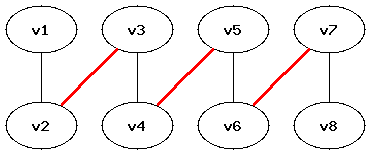
\includegraphics[scale=0.5]{1.png}

\textbf{Berge's theorem} (Claude Berge, 1957). Matching $M$ is greatest if and only if, for him there is no increasing the chain.

\textbf{Proof of necessity.} Suppose for a matching $M$ there is increasing chain $P$. We show how to go to the matching problem more power. Perform alternating matchings $M$ along this chain $P$ i.e. include in the matching edges $(v_1, v_2)$, $(v_3, v_4)$,..., $(v_ {k-1}, v_k)$ And remove from the matching edges $(v_2, v_3)$, $(v_4, v_5)$,..., $(v_ {k-2}, v_ {k-1})$. The result is likely to be received correctly matching, the power of which is one higher than the matching $M$ (Since we added $k / 2$ edges and remove $k/2-1$ edge).

\textbf{PROOF.} Suppose for a matching $M$ There is no magnifying circuit, we prove that it is the largest. Let $\overline M$ - Maximum matching. Consider the symmetric difference $\overline G = M \oplus \overline M$ (i.e. the set of edges belonging to either $M$ Or $\overline M$, But not both simultaneously). We show that $\overline G$ contains the same number of edges from $M$ and $\overline M$ (Because we excluded $\overline G$ only their common edge, then it will follow and $| M | = | \overline M |$ ). Note that $\overline G$ consists only of simple chains and cycles (because otherwise one would top two edges incident once a matching, which is impossible). Furthermore, the cycles can not have an odd length (for the same reason). Chain in $\overline G$ also can not have an odd length (otherwise it is the increasing chain for $M$, Which contradicts, or for $\overline M$, Which contradicts the maximality). Finally, in the even cycles and chains of even length in $\overline G$ ribs are alternately $M$ and $\overline M$, Which means that $\overline G$ occurs the same number of edges from $M$ and $\overline M$. As mentioned above, it follows that $| M | = | \overline M |$ i.e. $M$ is a maximum matching.

Berge's theorem provides the basis for the algorithm Edmonds - search-enhancing circuits and alternating along them, while increasing the chain are.

\subsection{ Edmonds' algorithm. Compressing Blossom }

The main problem is how to find the path increases. If the graph has cycles of odd length, then just run round in the depth / width not.

You can give a simple counter-example, when you run out of one of the peaks of the algorithm does not handle special cycles of odd length (in fact, Kuhn algorithm)finds increasing way, although it should. It is a cycle of length 3 with hanging on the edge of it, i.e. Count 1-2, 2-3, 3-1, 2-4, and the edge is taken in matching 3.2. Then, when you start from the top of one, if bypass goes first in the top two, then he "rested" in the top three, instead of finding magnifying circuit 1-3-2-4. True, in this example, you start from the top four Kuhn algorithm still finds this magnifying circuit.

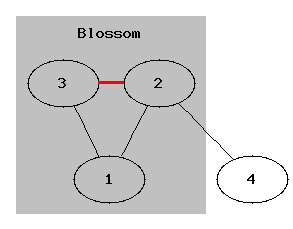
\includegraphics[scale=0.4]{2.png}

However, it is possible to construct a graph in which at a certain order in the list of adjacency algorithm Kuhn comes to a standstill. As an example, a graph with 6 vertices and 7 edges: 1-2, 1-6, 2-6, 2-4, 4-3, 1-5, 4-5. If we apply this algorithm for Kuhn, he will find a matching 1-6, 2-4, after which he will have to find magnifying chain 5-1-6-2-4-3, but could never find it (if from the top five he will go first to the 4, and then to 1, and when run from the top of the top 3, he will first 2 to 1, and only then to 6).

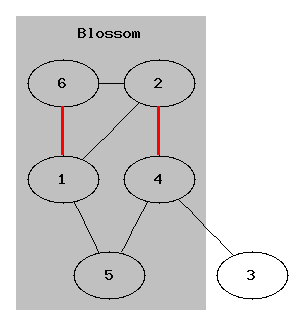
\includegraphics[scale=0.4]{3.png}

As we have seen in this example, the problem is that when released into the cycle of odd length can go crawl in a cycle in the wrong direction. In fact, we are interested in only the "rich" cycles, i.e. in which there is $k$ saturated edges, where the cycle length is $2k +1$. In this cycle, there is exactly one vertex not saturated edges of this cycle, we call it \textbf{a base} (base). To the top of the base is suitable alternating path of even (possibly zero) length, starting at the free (i.e. not owned by a matching of) the top, and this path is called the \textbf{stalk} (stem). Finally, the subgraph formed by the "rich" odd cycle, called the \textbf{flower} (blossom).

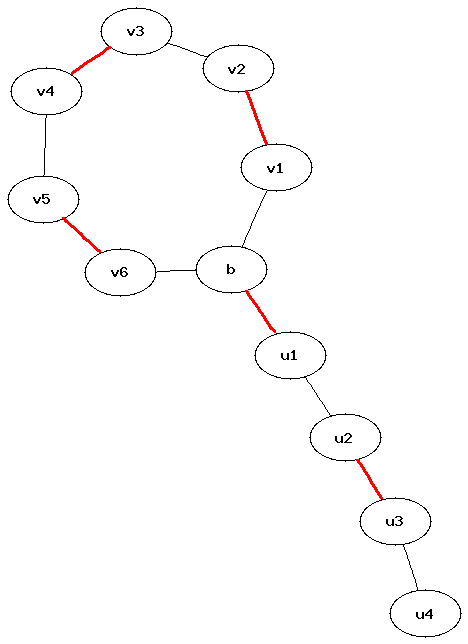
\includegraphics[scale=0.35]{4.png}

The idea of the algorithm Edmonds (Jack Edmonds, 1965) - in \textbf{compression flowers} (blossom shrinking). Compression of the flower - the contraction of the odd cycle in a pseudo-node (respectively, all the edges incident with this series, becoming incident pseudo-top). Edmonds' algorithm searches the graph all the flowers, compresses it, and then the graph is not "bad" cycles of odd length, and such a graph (called "surface" (surface) graph) can already look magnifying circuit simply by walking into the depth / width. After finding increasing the chain in the surface graph to "expand" the flowers, thereby restoring the magnifying circuit in the original graph.

However, not clear that after compression flower without breaking the graph, namely, that if the space $G$ there was increasing chain, then it exists in the graph $\overline G$ Obtained after compression of the flower, and vice versa.

\textbf{Edmonds' theorem.} Column $\overline G$ there is increasing chain if and only if there exists a chain increases in $G$.

\textbf{Proof.} So, let the graph $\overline G$ was obtained from the graph $G$ compression of a single flower (denoted $B$ cycle of a flower and a $\overline B$ the condensed vertex), we prove the theorem. First we note that it is sufficient to consider the case when the base of the flower is a free vertex (not belonging to matchings). Indeed, otherwise the base of the flower ends alternating path of even length, starting at the top of the free. Procheredovav matching along this path, the power matching will not change, and the base of the flower will become a free top. So, the proof, we may assume that the base of the flower is a free vertex.

\textbf{Proof of necessity.} Let the path $P$ is increased in a box $G$. If it does not pass through $B$, Then obviously it will increase in the graph $\overline G$. Let $P$ passes through $B$. Then we can without loss of generality assume that the path $P$ is a path $P_1$ Not passing over the tops $B$, Plus some way $P_2$ Running along the tops of $B$ and possibly other vertices. But then the way $P_1 + \overline B$ will be in the column by increasing the $\overline G$, As required.

\textbf{PROOF.} Let the path $\overline P$ is by increasing the in box $\overline G$. Again, if the path $\overline P$ does not pass through $\overline B$, The path $\overline P$ no change is increasing the way in $G$, So this case will not be considered.

We consider separately the case when $\overline P$ begins with compressed flower $\overline B$ i.e. has the form $(\overline B, c, \ldots)$. Then in flower $B$ there is a corresponding vertex $v$ Which is linked to (unsaturated) edge with $c$. It remains only to note that the base of the flower is always a even length alternating path to the top $v$. For all these reasons, we find that the way $P = (b, \ldots, v, c,...)$ is by increasing the in box $G$.

Let now the way $\overline P$ passes through the pseudo-vertex $\overline B$ But do not begin and end there. Then in $\overline P$ there are two edges passing through $\overline B$ Let it $(a, \overline B)$ and $(\overline B, c)$. One of them must necessarily belong matchings $M$ However, because base of the flower is not saturated, and all other vertices of the cycle of a flower $B$ saturated edges of the cycle, which is a contradiction. Thus, this case is simply not possible.

So, we reviewed all cases and in all of them showed the theorem Edmonds.

\textbf{General diagram of the Edmonds} becomes:

\begin{verbatim}
 void edmonds() {
    for(int i = 0 ; i < n ; ++ i )
        if(vertex i is not matching){
            int last_v = find_augment_path(i);
            if(last_v ! = - 1 )
                perform striping along the path from i to last_v;
        }
}
 
int find_augment_path(int root){
    preorder traversal:
         int v = tekuschaya_vershina;
         through all edges of v
             If you do find a cycle of odd length, squeeze it
             If it's a free vertex, return
             If it's not free at the top, then add
                 in turn adjacent to it in the matching
    return -1 ;
} 
\end{verbatim}
\subsection{ Efficient implementation }

Immediately evaluate asymptotics. A total of $n$ iterations, each of which crawls across a $O (m)$ In addition, surgery may be compression of the flowers - they can be $O (n)$. Thus, if we learn how to compress a flower $O (n)$, The general asymptotic behavior of the algorithm will $O (n \cdot (n + n ^ 2)) = O (n ^ 3)$.

The main difficulty is the shrink operation flowers. If you do them, directly combining the adjacency lists into one and removing it from the graph extra vertices, the asymptotic compression of one flower to $O (m)$ In addition, difficulties arise when "unfolding" of flowers.

Instead, we shall for each vertex $G$ maintain a pointer to the base of the flower, which she belongs (or yourself, if the node does not belong to flower). We have to solve two problems: the compression of the flower $O (n)$ when it is detected, and good preservation of all information for subsequent sequence which increases along the way.

Thus, one iteration of the algorithm is the Edmonds bypass wide, running from the top of a given free $\rm root$. Gradually builds a tree traversal in width, and the way it will be up to each vertex are interleaved by starting with a free vertex $\rm root$. For ease of programming will be put in place only those peaks, the distance to which the tree path is even (we call them the top even - that is the root of the tree, and the second ends of edges in the matching). The tree will be stored in an array of ancestors $\rm p []$ In which, for each odd vertex (i.e., the distance to which the tree is odd ways, that is the first ends of edges in the matching) will keep ancestor - even vertices. Thus, to set the path of the tree we have to turn to use arrays $\rm p []$ and $\rm match []$ Where $\rm match []$ - For each vertex has adjacent to it in matching or $-1$ If one is not.

Now it becomes clear how to detect cycles of odd length. If we are out of the current top $v$ during bypass wide come to a vertex $u$, Is the root $\rm root$ or belonging to a matching of the tree and the ways (i.e. $\rm p [match []]$ of which is not equal to 1), then we found a flower. Indeed, under these conditions, and the top $v$, And the top $u$ are even vertices. Distance from them to their lowest common ancestor has one parity, so we found a cycle of odd length.

Learn how to \textbf{compress the cycle.} So, we found an odd cycle when considering the edge $(v, u)$ Where $u$ and $v$ - Even vertices. Find their lowest common ancestor $b$, He will be the base of the flower. It is easy to see that the base is also an even vertex (because of the odd nodes in the tree path has only one son). However, it should be noted that $b$ - It may pseudovertex, so we actually find the base of the flower, which is the lowest common ancestor nodes $v$ and $u$. Implement immediately to find the lowest common ancestor (we are quite satisfied with the asymptotics $O (n)$ )

\begin{verbatim}
 int lca(int a, int b){
    bool used[MAXN]= { 0 } ;
    // from the top of a climb up from the roots, marking all even vertices
    for(;;){
        a = base[a];
        used[a]= true ;
        if(match[a]== - 1) break ; // come down to the root
        a = p[match[a]] ;
    }
    // rise from the top of b, until we find the marked vertex
    for(;;){
        b = base[b];
        if(used[b ]) return b ;
        b = p[match[b]] ;
    }
} 
\end{verbatim}
Now we need to identify the cycle - to walk from the tops $v$ and $u$ to the base $b$ flower. It would be more convenient if we are simply marks in a special array (call it $\rm blossom []$)Vertices belonging to the current flower. After that, we will need to reproduce the preorder traversal of the pseudo-top - just put in a preorder traversal of all the vertices lying on the cycle of the flower. Thus, we avoid the explicit join adjacency lists.

However, there is still one problem: correct recovery path after the bypass wide. For him, we maintain an array of ancestors $\rm p []$. But after the compression of flowers arises only problem preorder traversal continues immediately from all vertices cycle, including the odd, and the array of ancestors we have designed ways to restore the even vertices. Moreover, when there is a compressed column increases the chain through the flower, it will generally go through this cycle in such a direction that the tree ways this will be a downward spiral. However, all these problems are elegantly solved in this maneuver: compression cycle by placing all of its ancestors for even vertices (except base) to these "folks" point to the next peak in the cycle. For tops $u$ and $v$ If they also do not base their ancestors send pointers to each other. As a result, if the recovery-enhancing way we come to the cycle of the flower in the top of the odd, the path to the ancestors will be restored correctly, and will lead to the base of the flower (from which he will continue to recover normal).

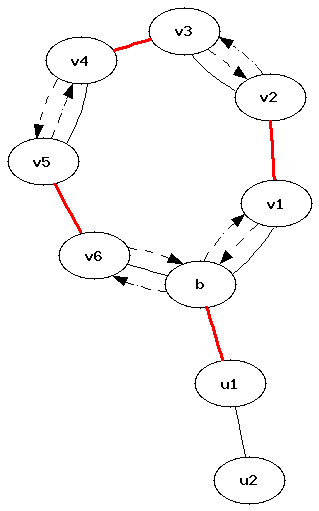
\includegraphics[scale=0.35]{5.png}

So, we are ready to implement compression of a flower:

\begin{verbatim}
int v, u ; // edge (v, u), the consideration of which was discovered by a flower
int b = lca(v, u);
memset(blossom, 0, sizeof blossom);
mark_path(v, b, u);
mark_path(u, b, v); 
\end{verbatim}
where the function $\rm mark \_path()$ is on the way from the top to the base of the flower, mark a special array $\rm blossom []$ for them $\rm true$ and affix the ancestors for even vertices. Parameter $\rm children$ - The son of the very top $v$ (With this option, we Loop the Loop in the ancestors).

\begin{verbatim}
void mark_path(int v, int b, int children){
    while(base[v]! = b){
        blossom[base[v]] = blossom[base[match[v]]]= true ;
        p[v]= children ;
        children = match[v];
        v = p[match[v]] ;
    }
} 
\end{verbatim}
Finally, we realize the basic function - $\rm find \_path ~ (int ~ root)$ That will look for a way of increasing the free vertex $\rm root$ and return the last vertex of the path, or $-1$ If increases the path was not found.

Initially perform initialization:

\begin{verbatim}
int find_path(int root){
    memset(used, 0, sizeof used);
    memset(p, - 1, sizeof p);
    for(int i = 0 ; i < n ; ++ i )
        base[i]= i ; 
\end{verbatim}
Next is a preorder traversal. Considering the next edge $(v, to)$ We have a few options:

\begin{itemize}

\item Edge nonexistent. By this we mean that $v$ and $to$ belong to a compressed pseudo-node(${\rm base} [v] == {\rm base} [to]$ ), So in the current column of the edge surface not. Besides this case, there is one case: when the edge $(v, to)$ already owned by the matching problem, since We assume that the vertex $v$ is an even vertex, then pass along this edge means the tree ways to rise to the top of ancestor $v$ That is unacceptable.

\begin{verbatim}
 if(base[v]== base[to]|| match[v]== to) continue ; 
\end{verbatim}
\item Edge closes a cycle of odd length, i.e. found a flower. As mentioned above, a cycle of odd length is detected under the condition:

\begin{verbatim}
 if(to == root || match[to]! = - 1 && p[match[to]] ! = - 1)
\end{verbatim}
In this case, you must compress the flower. It has already been examined in detail the process, here is its implementation:

\begin{verbatim}
 int curbase = lca(v, to);
memset(blossom, 0, sizeof blossom);
mark_path(v, curbase, to);
mark_path(to, curbase, v);
for(int i = 0 ; i < n ; ++ i )
    if(blossom[base[i]]){
        base[i]= curbase ;
        if(! used[i ]){
            used[i]= true ;
            q[qt ++]= i ;
        }
    } 
\end{verbatim}
\item Otherwise - it's "normal" edge, we proceed as in the normal search in width. The only fine - checking that this summit we have not yet visited, we must look not to the array $\rm used$ And an array $p$ - He filled in for odd vertices visited. If we are in the top $to$ still did not come, and it was unsaturated, we found magnifying circuit, ending at the top $to$, Return it.

\begin{verbatim}
if(p[to]== - 1){
    p[to]= v ;
    if(match[to]== - 1 )
        return to ;
    to = match[to];
    used[to]= true ;
    q[qt ++]= to ;
} 
\end{verbatim}
\end{itemize}

Thus, the complete implementation of the function $\rm find \_path()$ :

\begin{verbatim}
int find_path(int root){
    memset(used, 0, sizeof used);
    memset(p, - 1, sizeof p);
    for(int i = 0 ; i < n ; ++ i )
        base[i]= i ;
 
    used[root]= true ;
    int qh = 0, qt = 0 ;
    q[qt ++]= root ;
    while(qh < qt){
        int v = q[qh ++];
        for(size_t i = 0 ; i < g[v].size() ; ++ i){
            int to = g[v ][ i];
            if(base[v]== base[to]|| match[v]== to) continue ;
            if(to == root || match[to]! = - 1 && p[match[to]] ! = - 1){
                int curbase = lca(v, to);
                memset(blossom, 0, sizeof blossom);
                mark_path(v, curbase, to);
                mark_path(to, curbase, v);
                for(int i = 0 ; i < n ; ++ i )
                    if(blossom[base[i]]){
                        base[i]= curbase ;
                        if(! used[i ]){
                            used[i]= true ;
                            q[qt ++]= i ;
                        }
                    }
            }
            else if(p[to]== - 1){
                p[to]= v ;
                if(match[to]== - 1 )
                    return to ;
                to = match[to];
                used[to]= true ;
                q[qt ++]= to ;
            }
        }
    }
    return - 1 ;
} 
\end{verbatim}
Finally, we determine all the global arrays, and implementation of the main program for finding the greatest matching:

\begin{verbatim}
const int MAXN =... ; // the maximum number of nodes in the input box
 
int n ;
vector < int > g[MAXN];
int match[MAXN], p[MAXN], base[MAXN], q[MAXN];
bool used[MAXN], blossom[MAXN];
 
...
 
int main() {
    ... reading graph...
 
    memset(match, - 1, sizeof match);
    for(int i = 0 ; i < n ; ++ i )
        if(match[i]== - 1){
            int v = find_path(i);
            while(v ! = - 1){
                int pv = p[v],  ppv = match[pv];
                match[v]= pv,  match[pv]= v ;
                v = ppv ;
            }
        }
} 
\end{verbatim}
\subsection{ Optimization: constructing preliminary matchings }

As in the case of Algorithm Kuhn before performing Edmonds algorithm can be any simple algorithm to construct a pre-matching. For example, such a greedy algorithm: \begin{verbatim}
for(int i = 0 ; i < n ; ++ i )
    if(match[i]== - 1 )
        for(size_t j = 0 ; j < g[i].size() ; ++ j )
            if(match[g[i ][ j]] == - 1){
                match[g[i ][ j]] = i ;
                match[i]= g[i ][ j];
                break ;
            } 
\end{verbatim}
This optimization significantly (several times) will speed up the algorithm on random graphs.

\subsection{ Case of a bipartite graph }

In bipartite graphs are no cycles of odd length, and therefore, the code that performs the compression of the flowers, never executed. Mentally deleting all of the code that handle the compression of flowers, we get Algorithm Kuhn almost pure form. Thus, in the bipartite graphs Edmonds algorithm reduces to the algorithm Kuhn and works for $O (n m)$.

\subsection{ Further optimization }

All the above transactions with flowers thinly veiled operations with disjoint sets that can be done much more efficiently (see system of disjoint sets ). If we rewrite the algorithm using this structure, the asymptotic behavior of the algorithm drops to $O (n m)$. Thus, for arbitrary graphs, we have the same asymptotic estimate, as in the case of bipartite graphs (algorithm Kuhn), but significantly more complex algorithm.

\section{ Path cover in a directed acyclic graph }
Given a directed acyclic graph $G$. Need to cover it with the least number of ways, i.e., to find the minimum cardinality of the set of non-intersecting at the vertices of simple ways, such that each vertex belongs to a path.

\subsection{ Reduction to a bipartite graph }

Given a graph $G$ with $n$ vertices. We construct the corresponding bipartite graph $H$ the standard way, i.e.: in each part of the graph $H$ will $n$ vertices, which we denote by $a_i$ and $b_i$ respectively. Then, for each edge $(I, j)$ original graph $G$ hold the corresponding edge $(a_i, b_j)$.

Each edge $G$ corresponds to one edge $H$ And vice versa. If we look at $G$ either way $P = (v_1, v_2, \ldots, v_k)$, He is assigned a set of edges $(a_ {v_1}, b_ {v_2}), (a_ {v_2}, b_ {v_3}),..., (a_ {v_ {k-1}}, b_ {v_k})$.

Easier to understand is, if we add a "back" edges, that is form the graph $\overline H$ from graph $H$ adding edges of the form $(B_i, a_i), i = 1 \ldots N$. Then the path $P = (v_1, v_2, \ldots, v_k)$ in column $\overline H$ will correspond to the way $\overline Q = (a_ {v_1}, b_ {v_2}, a_ {v_2}, b_ {v_3},..., a_ {v_ {k-1}}, b_ {v_k})$.

Conversely, consider any path $\overline Q$ in column $\overline H$ Beginning in the first part and ending in the second one. Obviously, $\overline Q$ again takes the form $\overline Q = (a_ {v_1}, b_ {v_2}, a_ {v_2}, b_ {v_3},..., a_ {v_ {k-1}}, b_ {v_k})$, And it can be associated with the graph $G$ way $P = (v_1, v_2, \ldots, v_k)$. But there's a catch: $v_1$ could coincide with $v_k$, So the path $P$ result would be a cycle. However, by hypothesis graph $G$ acyclic, so it is not impossible (it is the only place that uses the acyclic graph $G$, However, the cyclic graphs general method described here can not be generalized.)

Thus, any simple path in the graph $\overline H$ Commencing on the first part and the second ending, you can assign a simple path in the graph $G$ And vice versa. But note that such a path in the graph $\overline H$ - Is \textbf{a matching} in a graph $H$. Thus, any path of $G$ can be associated with a matching in a graph $H$ And vice versa. Moreover, non-intersecting paths in $G$ correspond to disjoint matchings in $H$.

The last step. Note that the more ways there are in our set, the less these paths contain edges. That is, if there is $p$ disjoint paths that cover all $n$ vertices, then they both contain $r = n - p$ edges. So, to minimize the number of ways, we need to \textbf{maximize the number of edges} in them.

So, we have reduced the problem to finding a maximum matching in a bipartite graph $H$. After finding this matching (see Kuhn's algorithm ), we have to convert it into a set of paths in $G$ (This is a trivial algorithm, ambiguity does not arise here.) Some nodes may remain unsaturated matching, in this case, the answer must be the way to add a zero-length of each of these peaks.

\subsection{ Weighted case }

Weighted case is not much different from the unweighted, just in box $H$ appear on the edges of weight, and you want to find a matching has the least weight. Restoring response similar unweighted cases, we obtain a covering graph fewest ways and at equality - the lowest cost.

\section{ Tutte Matrix }
Tutte matrix - this elegant approach to the problem of \textbf{matching} in an arbitrary (not necessarily bipartite) graph. However, in the simplest form, the algorithm does not give yourself an edge belonging to a matching, and only the size of the maximum matching in a graph.

Below, we first consider the results obtained Tutte to ensure that a perfect matching (i.e. matching containing $n / 2$ edges, and thus saturating all $n$ vertices). After that, we consider the results obtained later Lovász, which already allows you to search the maximum size matching, and not just limited to the case of perfect matchings. Then show the result of Rabin and Vazirani, which indicated recovery of the matching algorithm (as a set of its constituent edges).

\subsection{ Definition }

Given a graph $G$ with $n$ vertices($n$ - Even).

Then the \textbf{matrix of Thatta} (Tutte) is the following matrix $n \times n$ :

$\begin{pmatrix}0 & x_{12} & x_{13} & \cdots & x_{1(n-1)} & x_{1n}\\
-x_{12} & 0 & x_{23} & \cdots & x_{2(n-1)} & x_{2n}\\
-x_{13} & -x_{23} & 0 & \cdots & x_{3(n-1)} & x_{3n}\\
\vdots & \vdots & \vdots & \ddots & \vdots & \vdots\\
-x_{1(n-1)} & -x_{2(n-1)} & -x_{3(n-1)} & \cdots & 0 & x_{(n-1)n}\\
-x_{1n} & -x_{2n} & -x_{3n} & \cdots & -x_{(n-1)n} & 0
\end{pmatrix}
 $

where $x_ {ij}$($1 \le i <j \le n$)- Either independent variable corresponding to the edge between vertices $i$ and $j$ Or identically zero, if the edges between vertices not.

Thus, in the case of a complete graph with $n$ vertices matrix contains Thatta $n (n-1) / 2$ independent variables, if any edge in the graph are missing, then the corresponding elements of Thatta become zeros. In general, the number of variables in the matrix corresponds to the number of Tutte edges.

Thatta antisymmetric matrix (skew).

\subsection{ Tutte's theorem }

Consider the determinant $\det (A)$ Tutte matrix. Generally speaking, a polynomial in the variables $x_ {ij}$.

\textbf{Tutte's theorem} states that in the graph $G$ there is a perfect matching if and only if the polynomial $\det (A)$ is not identically zero (i.e., has at least one term with a nonzero coefficient). Recall that a matching is called perfect if it saturates all the vertices, i.e., its power is $n / 2$.

Canadian mathematician William Thomas Tutte (William Thomas Tutte) first pointed out the close relationship between matchings in graphs and the determinant of (1947). A simpler form of this connection later discovered Edmonds (Edmonds) in the case of bipartite graphs (1967). Randomized algorithms for finding the value of the maximum matching and matching of edges themselves were offered later, respectively, Lovász (Lovasz) (in 1979), and Rabin (Rabin) and Vazirani (Vazirani) (in 1984).

\subsubsection{ Practical application: a randomized algorithm }

Directly apply the theorem of Tutte, even the problem of testing the existence of a perfect matching is impractical. The reason for this is that when calculating the determinant character (i.e. in the form of polynomials on the variables $x_ {ij}$)Interim results are polynomials containing $O (n ^ 2)$ variables. Therefore the calculation of the determinant of Thatta in symbolic form would require an inordinate amount of time.

Hungarian mathematician László Lovász (Laszlo Lovasz) was the first who pointed out the possibility of applying the \textbf{randomized} algorithm to simplify calculations.

The idea is very simple: replace all the variables $x_ {ij}$ random numbers:

$x_ {ij} = {\rm rand}().$

Then, if a polynomial $\det (A)$ was identically zero, after such a change, and it will remain zero, but if it was a non-zero, then for such a random number replace the likelihood that he will turn to zero, is fairly small.

It is clear that such a test (the value of random values ​​and the calculation of the determinant $\det (A)$)If it is wrong, it is only in one direction, may report the absence of perfect matchings, when in fact it exists.

We can repeat the test several times, substituting the values ​​of the variables as random numbers, and every restart we get more and more confident that the test gave the correct answer. In practice, in most cases a single test to determine whether there is a perfect matching in a graph or not, some of these tests give the already very high probability.

To estimate the \textbf{probability of error} can use Lemma Schwarz-Zippelya (Schwartz-Zippel), which states that the probability of the vanishing non-zero polynomial $P$$k$ Second degree when substituted as random variables, each of which can take $s$ option values ​​- this probability satisfies:

${\rm Pr} [P (r_1, \ldots, r_k) = 0] \le \frac {k} {s}.$

For example, using the standard function of random numbers C++ $\rm rand()$ we find that the probability is at $n = 300$ amounts to about one percent.

\textbf{Asymptotics of the} solution turns out to be $O (n ^ 3)$ (Using, for example, the Gauss algorithm ), multiplied by the number of iterations of the test. It should be noted that the asymptotic solution is far behind the decision algorithm Edmonds compression flowers, but in some cases more preferred due to the ease of implementation.

\textbf{Reestablish} itself as a perfect matching set of edges is more complex. The easiest, though slow, option would be to restore this matching one edge: loop through the first edge of the answer, select it so that there remains a graph perfect matching, etc.

\subsubsection{ Proof of Tutte }

It is good to understand the proof of this theorem, we first consider a simple result - Edmonds obtained for the case of bipartite graphs.

Edmonds theorem
Consider a bipartite graph, in which each part on $n$ vertices. Form the matrix $B$$n \times n$ In which, by analogy with the matrix Thatta, $b_ {ij}$ a single independent variable, if an edge $(I, j)$ is present in the graph, and is identically zero otherwise.

This matrix is ​​similar to the Tutte matrix, but the matrix Edmonds has half the difference, and each edge here has only one cell in the matrix.

Prove the following \textbf{theorem:} the determinant $\det (B)$ different from zero if and only if in a bipartite graph contains a perfect matching.

\textbf{Proof.} We expand the determinant according to its definition, the sum over all the permutations:

$\det(B)=\sum_{\pi\in S_{n}}{\rm sgn}(\pi)\cdot b_{1,\pi_{1}}\cdot\ldots\cdot b_{n,\pi_{n}}$

Note that since the non-zero elements of the matrix $B$ - The various independent variables, in this sum, all nonzero terms are different, and therefore any reductions in the summation occurs. It remains to note that any non-zero term in the sum means the tops of disjoint set of edges, that is a perfect matching. Conversely, any perfect matching corresponds to a non-zero term in this sum. Coupled with the above, this proves the theorem.

Properties antisymmetric matrices
To prove the theorem of Tutte to use several well-known facts of linear algebra on the properties of antisymmetric matrices.

\textbf{First} (this fact will not be useful, but it is interesting in itself), if an antisymmetric matrix of odd size, then the determinant is always zero (Theorem Jacobi (Jacobi)). It is sufficient to note that the antisymmetric matrix satisfies $A ^ T =-A$ And now we get the chain of equalities

$\det (A) = \det (A ^ T) = \det (-A) = (-1) ^ n \det (A),$

which implies that for odd $n$ determinant must be equal to zero.

\textbf{Second,} it appears that in the case of anti-symmetric matrices of even size of their determinant can always be written as the square of a polynomial in the variables, the elements of this matrix (called the Pfaffian polynomial (pfaffian), and the result belongs Muir (Muir)):

$\det (A) = {\rm Pf} ^ 2 (A).$

\textbf{Third,} the Pfaffian is not an arbitrary polynomial, and the sum of the form:

${\rm Pf}(A)=\frac{1}{2^{n}n!}\sum_{\pi\in S_{n}}{\rm sgn}(\pi)\cdot a_{\pi_{1},\pi_{2}}\cdot a_{\pi_{3},\pi_{4}}\cdot\ldots\cdot a_{\pi_{n-1},\pi_{n}}$

Thus, each term in the Pfaffian - is the product of such $n / 2$ elements of their indices in the aggregate represent a partition of $n$ on $n / 2$ pairs. Before each term has a factor, but it kind of does not interest us here.

The proof of Tutte
Using the second and third property in the previous paragraph, we see that the determinant $\det (A)$ Tutte matrix is ​​the square of the sum of the terms of this form, that each term - the product of the entries whose indices are not repeated, and cover all the numbers on the $1$ to $n$. So, again, as in the proof of Edmonds, every non-zero term in this sum corresponds to perfect matching in a graph, and vice versa.

\subsection{ Lovasz Theorem: generalization to find the maximum matching size }

\subsubsection{ Formulation }

Thatta \textbf{rank} equal to twice the size of \textbf{the maximum matching} in this graph.

\subsubsection{ Application }

To apply this theorem in practice, you can use the same technique of randomization as in the above algorithm for matrix Thatta, namely substitute variables random values, and find the rank obtained by the numerical matrix. Rank, again, we look for $O (n ^ 3)$ using a modified Gaussian algorithm, see here.

However, it should be noted that the algorithm given in the previous lemma Schwarz-Zippelya applicable explicitly, and intuitively it seems that the probability of error is higher here. But it is claimed (see the work Lovasz (Lovasz)), that is the probability of error (i.e., that the rank of the resulting matrix will be less than twice the size of the maximum matching) does not exceed $\frac {n} {s}$ (Where $s$ As above, indicates the size of the set, from which the random numbers).

\subsubsection{ Proof }

The proof will follow from a single \textbf{property,} from linear algebra. Let an antisymmetric matrix $A$ size $n \times n$ And let the set $S$ and $T$ - Any two subsets $\{1, \ldots, n \}$, And the sizes of these sets are the same. We denote $A_ {ST}$ matrix obtained from $A$ only the rows with indices of $S$ and columns with indices $T$. Then we have:

$\det(A_{SS})\cdot\det(A_{TT})=\det(A_{ST})\cdot\det(A_{TS})$

We show how this property to establish a \textbf{correspondence} between the rank of the matrix Thatta $A$ and the value of the maximum matching.

On the one hand, consider the graph $G$ a maximum matching, and the set of vertices by their saturable $U$. Then the determinant $\det (A_ {UU})$ different from zero (by a theorem of Tutte). Investigator, the rank Tutte at least not less than twice the size of the maximum matching.

Conversely, let the rank of $A$ is $r$. This means that you have found a submatrix $A_ {ST}$ Where $| S | = | T | = r$ Determinant is not zero. But according to the above property, this means that one of the matrices $A_ {SS}$, $A_ {TT}$ has a nonzero determinant, by Theorem Thatta means that the subgraph induced by the set of vertices $S$ or $T$, There is a perfect matching (and equal to the value of $r / 2$ ). Consequently, the rank can not be greater than the maximum matching, which completes the proof.

\subsection{ Rabin-Vazirani algorithm for finding the maximum matching }

This algorithm is a further generalization of the previous two theorems, and allows, in contrast, the issue is not only the magnitude of the maximum matching, but the very edge, combined.

\subsubsection{ Theorem statement }

Let the graph there is a perfect matching. Then its Tutte matrix is ​​nonsingular, i.e. $\det (A) \ne 0$. To generate it, as described above, random numerical matrix $B$. Then, with high probability, $(B ^ {-1}) _ {ji} \ne 0$ if and only if the edge $(I, j)$ included in any perfect matching.

(Here $B ^ {-1}$ denotes the inverse matrix of $B$. It is assumed that the determinant of $B$ different from zero, so the inverse exists.)

\subsubsection{ Application }

This theorem can be used to restore the edges themselves maximal matching. Will first have to select a subgraph, which contains the desired maximal matching (this can be done in parallel with the rank of the search algorithm).

After that the problem reduces to the search for the perfect matching of the numerical matrix obtained from the matrix of Thatta. Here we apply the theorem of Rabin-Vazirani - find the inverse matrix (which can be modified algorithm for Gaussian $O (n ^ 3)$ ), We find in it any nonzero element, remove it from the graph, and repeat the process. Asymptotics of the solutions will not be the fastest - $O (n ^ 4)$, But instead we get easy solutions (compared, for example, the compression algorithm Edmonds flowers ).

\subsubsection{ Proof }

Recall the well-known formula for the elements of the inverse matrix $B ^ {-1}$ :

$(B^{-1})_{ji}=\frac{{\rm adj}(B)_{i,j}}{\det(B)}$

where by ${\rm adj} (B) _ {i, j}$ indicated cofactor, i.e. this number $(-1) ^ {I + j}$ Multiplied by the determinant of the matrix obtained from $B$ Disposal $i$ -Th row and $j$ Th column.

It follows at once that the element $(B ^ {-1}) _ {ji}$ different from zero if and only if the matrix $B$ with strike- $i$ Th row and $j$ -Th column has a nonzero determinant, that by applying Tutte's theorem implies a high probability that the graph without vertices $i$ and $j$ there is still a perfect matching.

\subsection{ Literature }

\begin{itemize} \item William Thomas Tutte. \textbf{The Factorization of Linear Graphs} [1946] \item Laszlo Lovasz. \textbf{On Determinants, Matchings and Random Algorithms} [1979] \item Laszlo Lovasz, MD Plummer. \textbf{Matching Theory} [1986] \item Michael Oser Rabin, Vijay V. Vazirani. \textbf{Maximum matchings in general graphs through randomization} [1989] \item Allen B. Tucker. \textbf{Computer Science Handbook} [2004] \item Rajeev Motwani, Prabhakar Raghavan. \textbf{Randomized Algorithms} [1995] \item AC Aitken. \textbf{Determinants and matrices} [1944] \end{itemize}

\section{ Edge connectivity properties }
\subsection{ Definition }

Given a undirected graph $G$ with $n$ vertices and $m$ edges.

\textbf{Branch Connectivity} $\lambda$ column $G$ is the smallest number of edges that must be removed in order to count no longer connected.

For example, to disconnected graph edge-connectivity zero. For a connected graph with a single edge-connectivity of the bridge is one.

A set $S$ edges \textbf{separating} vertices $s$ and $t$, If you delete these edges from the graph vertices $u$ and $v$ are in different connected components.

Clearly, the edge-connectivity of a graph is equal to the minimum of the minimum number of edges that separate the two peaks $s$ and $t$, Taken among all pairs $(S, t)$.

\subsection{ Properties }

\subsubsection{ Whitney ratio }

\textbf{Ratio Whitney (Whitney) (1932)} between the Branch Connectivity $\lambda$, the vertex connectivity $\kappa$ and the smallest degree of a vertex $\Delta$ :

$\kappa \le \lambda \le \Delta.$

\textbf{Proof.}

We first prove the first inequality: $\kappa \le \lambda$. Consider this set of $\lambda$ edges, making the graph connected. If we take each of these edges on one end (either of the two) and remove from the graph, thereby using $\le \lambda$ remote nodes (since the same vertex could meet twice) we make the graph disconnected. Thus, the $\kappa \le \lambda$.

Let us prove the second inequality: $\lambda \le \Delta$. Consider a vertex of minimal degree, then we can remove all $\Delta$ allied edges and thus to separate this from the rest of the top of the graph. Consequently, the $\lambda \le \Delta$.

Interestingly, the Whitney inequality \textbf{can not be improved:} i.e. for all triples that satisfy this inequality, there is at least one corresponding graph. See the problem, "Graphing with these vertex and edge connections and lowest vertex degree".

\subsubsection{ Ford-Fulkerson theorem }

\textbf{Ford-Fulkerson theorem} (1956):

For any two vertices of the largest number of edge-disjoint chains connecting them, equal to the minimum number of edges separating these peaks.

\subsection{ Finding the edge connectivity }

\subsubsection{ A simple algorithm based on maximum flow }

This method is based on the theorem of Ford-Falekrsona.

We have to go through all pairs of vertices $(S, t)$ And between each pair to find the largest number of edge disjoint paths. This value can be found by using the maximum flow algorithm: we do $s$ source, $t$ - Drain and capacity of each edge we put equal to 1.

Thus, the pseudo-code algorithm is:

\begin{verbatim}
int ans = INF ;
for(int s = 0 ; s < n ; ++ s )
    for(int t = s + 1 ; t < n ; ++ t){
        int flow =... value of the maximum flow from s to t...
        ans = min(ans, flow);
    } 
\end{verbatim}
Asymptotic behavior of the algorithm using edmonds\_karp {Edmonds-Karp algorithm of finding the maximum flow is obtained} $O (n ^ 2 \cdot n m ^ 2) = O (n ^ 3 m ^ 2)$ However it should be noted that hidden in the asymptotic constant is very small, since it is practically impossible to create a graph algorithm to find the maximum flow slowly worked once for all the drain and source.

Particularly fast, this algorithm will work on random graphs.

\subsubsection{ A special algorithm }

Using streaming terminology, this problem - it is the problem of finding \textbf{the global minimum cut.}

To solve it, a special algorithm. This site presents one of which - Curtains-Wagner algorithm running in time $O (n ^ 3)$ or $O (n m)$.

\subsection{ Literature }

\begin{itemize}

\item Hassler Whitney. \textbf{Congruent Graphs and the Connectivity of Graphs} [1932]

\item Frank Harary. \textbf{Graph Theory} [2003]

\end{itemize}

\section{ Vertex connectivity properties }
\subsection{ Definition }

Given a undirected graph $G$ with $n$ vertices and $m$ edges.

\textbf{Vertex connectivity} $\lambda$ column $G$ is the smallest number of vertices to be deleted, the graph is no longer connected.

For example, to disconnected graph vertex connectivity is zero. For a connected graph with a single point of articulation vertex connectivity is one. For a complete graph vertex connectivity is set equal $n-1$ (As which pair of vertices we may choose, even the removal of all remaining vertices will not make them non-connected). For all graphs, but complete, vertex connectivity is at most $n-2$ - Because you can find a pair of nodes between which there is no edge, and remove all other $n-2$ top.

A set $S$ vertices \textbf{shared} vertices $s$ and $t$, If you delete these vertices of the graph vertices $u$ and $v$ are in different connected components.

It is clear that the vertex connectivity of the graph is the minimum of the minimum number of vertices separating two vertices $s$ and $t$, Taken among all pairs $(S, t)$.

\subsection{ Properties }

\subsubsection{ Whitney ratio }

\textbf{Ratio Whitney (Whitney) (1932)} between the Branch Connectivity $\lambda$, The vertex connectivity $\kappa$ and the smallest degree of a vertex $\Delta$ :

$\kappa \le \lambda \le \Delta.$

\textbf{Proof.}

We first prove the first inequality: $\kappa \le \lambda$. Consider this set of $\lambda$ edges, making the graph connected. If we take each of these edges on one end (either of the two) and remove from the graph, thereby using $\le \lambda$ remote nodes (since the same vertex could meet twice) we make the graph disconnected. Thus, the $\kappa \le \lambda$.

Let us prove the second inequality: $\lambda \le \Delta$. Consider a vertex of minimal degree, then we can remove all $\Delta$ allied edges and thus to separate this from the rest of the top of the graph. Consequently, the $\lambda \le \Delta$.

Interestingly, the Whitney inequality \textbf{can not be improved:} i.e. for all triples that satisfy this inequality, there is at least one corresponding graph. See the problem, "Graphing with these vertex and edge connections and lowest vertex degree".

\subsection{ Finding the vertex connectivity }

Iterate through a pair of vertices $s$ and $t$ And find the minimum number of vertices, which must be removed to separate $s$ and $t$.

To do this, each vertex \textbf{is bifurcated:} i.e. each vertex $i$ create two copies - one $i_1$ for incoming edges, the other $i_2$ - For leaving, and the two copies are connected to each other by an edge $(I_1, i_2)$.

Each edge $(u, v)$ the original graph in the modified network will become a two edges: $(u_2, v_1)$ and $(v_2, u_1)$.

All edges to put the capacity of unity. We now find the maximum flow in the graph between the source $s$ and the drain $t$. By construction of the graph, and it will be a minimum number of vertices needed to separate $s$ and $t$.

Thus, if the search for the maximum flow algorithm we choose the Edmonds-Karp, who works for the time $O (n m ^ 2)$, The general asymptotic behavior of the algorithm will $O (n ^ 3 m ^ 2)$. However, the constant hidden in the asymptotic behavior, is very small: as to make a graph on which the algorithm would have worked a long time at any pair of source-drain is almost impossible.

\section{ Graph construction with stated values ​​of vertex and edge connectivity }
Given values $\kappa$, $\lambda$, $\Delta$ - Are, respectively, the vertex connectivity, edge-connectivity and the minimum degree of the vertices. Required to construct a graph which would have the specified values, or to say that this graph does not exist.

\subsection{ Whitney ratio }

\textbf{Ratio Whitney (Whitney) (1932)} between the Branch Connectivity $\lambda$, the vertex connectivity $\kappa$ and the smallest degree of a vertex $\Delta$ :

$\kappa \le \lambda \le \Delta.$

\textbf{Proof.}

We first prove the first inequality: $\kappa \le \lambda$. Consider this set of $\lambda$ edges, making the graph connected. If we take each of these edges on one end (either of the two) and remove from the graph, thereby using $\le \lambda$ remote nodes (since the same vertex could meet twice) we make the graph disconnected. Thus, the $\kappa \le \lambda$.

Let us prove the second inequality: $\lambda \le \Delta$. Consider a vertex of minimal degree, then we can remove all $\Delta$ allied edges and thus to separate this from the rest of the top of the graph. Consequently, the $\lambda \le \Delta$.

Interestingly, the Whitney inequality \textbf{can not be improved:} i.e. for all triples that satisfy this inequality, there is at least one corresponding graph. We prove it constructively, showing how to build the boxes.

\subsection{ Decision }

Check whether the data of $\kappa$, $\lambda$ and $\Delta$ Whitney ratio. If not, then there is no answer.

Otherwise, we construct the graph itself. It will consist of $2 (\Delta + 1)$ peaks, with the first $\Delta + 1$ vertices form fully connected subgraph, and the second $\Delta + 1$ the top also form a full mesh subgraph. In addition, we join the two parts $\lambda$ edges so that the first part of these edges are adjacent $\lambda$ vertices in the other part - $\kappa$ tops. It is easy to verify that the resulting graph will have the necessary characteristics.

\section{ Inverse problem of single-source shortest paths }
There is a weighted undirected multigraph G of N vertices and M edges. Dan array P [1.. N] and to indicate the initial vertex of S. Want to change the weights of the edges so that all IP [I] was equal to the length of the shortest path from S to I, and the sum of all the changes (sum of absolute changes in the weights of edges) would be minimal. If this is not possible, then the algorithm should output "No solution". Do negative edge weight is prohibited.

\subsection{ The solution }
We will solve this problem in linear time, just sorting out all the edges (i.e., in one pass).

Suppose that at the current stage, we consider an edge from vertex A to vertex B length R. We assume that the vertex A is all the conditions are met (i.e. the distance from S to A is indeed equal to P [A]), and will check that the conditions for the vertex B. We have several options for the situation:

\begin{itemize} \item 1. \textbf{P [A] + R <P [B]} 
This means that we found a way shorter than it should be. Since P [A] and P [B], we can not change, we have to extend the current edge (regardless of the other edges), namely, execute: 
R + = P [B] - P [A] - R. 
In addition, it means that we have already found the way to the top of the B S, whose length is equal to the desired value P [B], so the next steps we will not have any shortening of the edge (see Option 2). \item 2. \textbf{P [A] + R>= P [B]} 
This means that we have found a way, longer than required. Since there may be several ways, we have to choose among all these paths (edges) that will require the least change. Again, if we lengthened a an edge to the vertex B (option 1), the fact that we built the shortest way to the top of B, and thus shorten the no edge will not have to. Thus, for each vertex, we must keep an edge, which is going to be shortened, i.e. edge with the smallest weight changes. \end{itemize}
So, just sorting through all the edges, and having considered the situation for each edge (with the O (1)), we solve the inverse problem in linear time SSSP.

If at any point we are trying to change an altered edge, then, obviously, can not do that, and it should give "No solution". In addition, some of the vertices can be never achieved the desired estimate the shortest path, then the answer would also be "No solution". In all other cases (except, of course, is clearly incorrect values ​​in the array P, i.e., P [S]! = 0 or negative) response will exist.

\subsection{ Implementation }
The program displays "No solution", if there is no solution, otherwise, the first line of the minimum amount of changes in the weights of edges, while the following M lines - the new edge weights.

\begin{verbatim}
 const int INF = 1000 * 1000 * 1000;
 int n, m;
 vector <int> p (n);

 bool ok = true;
 vector <int> cost (m), cost_ch (m), decrease (n, INF), decrease_id (n, -1);
 decrease [0] = 0;
 for (int i = 0; i <m;++ i) {
     int a, b, c; // current edge (a, b) the price of c
     cost [i] = c;

     for (int j = 0; j <= 1;++ j) {
         int diff = p [b] - p [a] - c;
         if (diff> 0) {
             ok & = cost_ch [i] == 0 | | cost_ch [i] == diff;
             cost_ch [i] = diff;
             decrease [b] = 0;
         }
         else
             if (-diff <= c &&-diff <decrease [b]) {
                 decrease [b] =-diff;
                 decrease_id [b] = i;
             }
         swap (a, b);
     }
 }

 for (int i = 0; i <n;++ i) {
     ok & = decrease [i]! = INF;
     int r_id = decrease_id [i];
     if (r_id! = -1) {
         ok & = cost_ch [r_id] == 0 | | cost_ch [r_id] ==-decrease [i];
         cost_ch [r_id] =-decrease [i];
     }
 }

 if (! ok)
     cout << "No solution";
 else {
     long long sum = 0;
     for (int i = 0; i <m;++ i) sum + = abs (cost_ch [i]);
     cout << sum << '\n';
     for (int i = 0; i <m;++ i)
         printf ("% d", cost [i] + cost_ch [i]);
 } 
\end{verbatim}
\section{ Inverse problem of minimum spanning tree }
Given a weighted undirected graph G with N vertices and M edges (no loops or multiple edges). It is known that the graph is connected. Also specify that the skeleton of the graph T (i.e., selected N-1 edges that form a tree with N vertices). Want to change the weights of the edges in such a way that the skeleton of T is the minimum spanning tree of the graph (more precisely, one of the minimum spanning tree), and make it so that the total change of all was the smallest scales.

\subsection{ Decision }
\textbf{Reduce the} problem of inverse-MST to the problem min-cost-flow, more precisely, \textbf{to the problem of the dual min-cost-flow} (in the sense of the duality of linear programming), and then solve the last problem.

So, let G be a graph with N vertices, M edges. Weight of each edge is denoted by C i. Assume without loss of generality that the edges with the numbers from 1 to N-1 are edges of T.

\subsubsection{ A necessary and sufficient condition for MST }
Let there be given a skeleton S (not necessarily minimal).

We first introduce the notation. Consider some edge j, does not belong to S. Obviously, the graph S has a single path connecting the ends of the edge, i.e., the only path connecting the ends of j and consisting only of the edges belonging to S. \textbf{Let P [j]} the set of edges that make up the way for the j-th rib.

In order to be a skeleton S is minimal \textbf{if and only if:}

\begin{verbatim}
 C i <= C j for all j ∉ S and every i ∈ P [j] 
\end{verbatim}
It can be noted that, as \textbf{in our problem} belongs to the edge skeleton T 1.. N-1, we can write this condition as follows:

\begin{verbatim}
 C i <= C j for all j = N.. M and every i ∈ P [j]
 (All of which i lie in the range 1.. N-1) 
\end{verbatim} \subsubsection{ Count the ways }
Count the ways the concept is directly related to the previous theorem.

Let there be given a skeleton S (not necessarily minimal).

Then \textbf{count the ways H} for a graph G is the following graph:

\begin{itemize} \item It contains M nodes, each node in H uniquely corresponds to some edge in G. \item Bipartite graph H. In his first share are top i, which correspond to the edges in G, belonging to the skeleton of S. Accordingly, in the second part are the vertices j, which correspond to the edges not belonging to S. \item An edge is drawn from node i to j if and only if i belongs to P [j]. 
In other words, for each vertex j of the second part, it includes all the vertices of the edges in the first part corresponding to a plurality of ribs P [j]. \end{itemize}
In the case of \textbf{our problem,} we can slightly simplify the description of the graph of ways:

\begin{verbatim}
 edge (i, j) exists in H, if i ∈ P [j], j = N.. M, i = 1.. N-1 
\end{verbatim} \subsubsection{ Mathematical formulation of the problem }
Purely formal \textbf{problem inverse-MST} is written as follows:

\begin{verbatim}
 find an array A [1.. M] such that
 C i + A i <= C j + A j for all j = N.. M and every i ∈ P [j] (i in 1.. N-1)
 and to minimize the amount of | A 1 | + | A 2 | +...  + | A m | 
\end{verbatim}
here under the desired array of A, we mean those values ​​that must be added to the balance of edges (i.e., solving the problem of inverse-MST, we replace the weight of each edge of C i i the value of C i + A i).

Obviously, it makes no sense to increase the weight of the edges belonging to T, i.e.,

\begin{verbatim}
 A i <= 0, i = 1.. N-1 
\end{verbatim}
it makes no sense to shorten the edges not belonging to T:

\begin{verbatim}
 A i>= 0, i = N.. M 
\end{verbatim}
(Because otherwise we will only worsen the response)

Then we can \textbf{simplify} the problem a bit by removing the sum of modules:

\begin{verbatim}
 find an array A [1.. M] such that
 C i + A i <= C j + A j for all j = N.. M and every i ∈ P [j] (i in 1.. N-1)
 A i <= 0, i = 1.. N-1,
 A i>= 0, i = N.. M,
 and to minimize the amount of A n +...  + A m - (A 1 +... + A n-1) 
\end{verbatim}
Finally, we must change the "minimize" to "maximize", and in the amount of change all signs to the contrary:

\begin{verbatim}
 find an array A [1.. M] such that
 C i + A i <= C j + A j for all j = N.. M and every i ∈ P [j] (i in 1.. N-1)
 A i <= 0, i = 1.. N-1,
 A i>= 0, i = N.. M,
 and to maximize the amount of A 1 +...  + A n-1 - (A n +... + A m) 
\end{verbatim} \subsubsection{ Reduction of the inverse-MST, the dual problem of assignment }
Formulation of the inverse-MST, which we have just given, is the formulation of a \textbf{linear programming} problem with unknown A 1.. A m.

Applying the classical method - consider its \textbf{dual} problem.

By definition, to obtain a dual problem, you need to compare each inequality dual variable X ij, roles of the objective function (which had to be minimized), and the coefficients on the right side, change the signs "<=" on ">=", and vice versa, change the maximization to minimize.

So, \textbf{its dual inverse-MST} problem:

\begin{verbatim}
 find all X ij for each (i, j) \in H, such that:
 all X ij>= 0,
 for each i = 1.. N-1 \sum X ij for all j: (i, j) \in H <= 1,
 for each j = N.. M \sum X ij for all i: (i, j) \in H <= 1,
 and minimize \um X ij (C j - C i) for all (i, j) \in H 
\end{verbatim}
The last task is a \textbf{task assignment:} we need in the box to select multiple paths H edges so that no edge is disjoint from the other at the top, and the sum of weights of the edges (the weight of an edge (i, j) is defined as the C j - C i) to be minimal.

Thus, the \textbf{dual problem inverse-MST is equivalent to the assignment problem.} If we can solve the dual problem of the assignment, we will automatically solve the problem of inverse-MST.

\subsubsection{ Solution to the dual assignment problem }
First, we'll pay some attention to the special case of the assignment problem, which we got. First, it is an unbalanced assignment problem, because in the same part is N-1 vertices, and the other - M vertices, i.e., in general, the number of vertices in the second one more on the whole order. To solve such a dual assignment problem is a specialized algorithm that decides it for $O(N^3)$, but here, this algorithm will not be considered. Second, such a task assignment include assignment problems with weighted vertices: the edge weights are set equal to 0, the weight of each vertex of the first part is set equal to-C i, of the second part - equal to C j, and solving a problem is to be the same most.

We will solve the problem of the dual problem of the nominations by the \textbf{modified algorithm min-cost-flow,} which will find the minimum cost flow and at the same time the solution of the dual problem.

\textbf{Reduce the} problem of appointments to the problem min-cost-flow very easily, but for the sake of completeness, we will describe the process.

Add to the graph source s and sink t. From s to each vertex of the first part will hold an edge with capacity = 1 and the value 0. From each vertex of the second part to t hold an edge with capacity = 1 and the value 0. Capacity of all edges between the first and second installments also set to 1.

Finally, the modified algorithm for min-cost-flow (described below) to work, you need to \textbf{add an edge from s to t} with capacity = N +1 and the value 0.

\subsubsection{ Modified algorithm min-cost-flow for the assignment problem }
Here we consider the \textbf{successive shortest path algorithm with potentials,} which resembles the usual algorithm min-cost-flow, but also uses the concept of \textbf{potential,} which by the end of the algorithm will contain a \textbf{solution to the dual problem.}

Introduce some notation. For each edge (i, j) is denoted by U ij its capacity through C ij - its value, after F ij - flow along this edge.

Also introduce the notion of potential. Each vertex has its potential PI i. The residual value of an edge CPI ij is defined as:

\begin{verbatim}
 CPI ij = C ij - PI i + PI j 
\end{verbatim}
At any time of the algorithm \textbf{capabilities are such} that the following conditions are met:

\begin{verbatim}
 if F ij = 0, the CPI ij>= 0
 if F ij = U ij, then the CPI ij <= 0
 otherwise CPI ij = 0 
\end{verbatim}
The algorithm starts with a zero flow, and we need to find some initial potential values ​​that satisfy the above conditions. It is easy to see that this method is one of the possible solutions:

\begin{verbatim}
 PI j = 0 for j = N.. M
 PI i = min C ij, where (i, j) ∈ H
 PI s = min PI i, where i = 1.. N-1
 PI t = 0 
\end{verbatim}
Actually, the algorithm min-cost-flow consists of several iterations. \textbf{At each iteration,} we find the shortest path from s to t in the residual network, and the weights of edges using the residual value of CPI. Then we increase the flow along the path found by one, and update capabilities as follows:

\begin{verbatim}
 PI i - = D i 
\end{verbatim}
where D i - found the shortest distance from s to i (again, in the residual network with edge weights CPI).

Sooner or later we will find the path from s to t, which consists of a single edge (s, t). Then after this iteration, we need to \textbf{complete the} algorithm: indeed, if we do not stop the algorithm, it will already be on the way to a non-negative value, and add them to the answer is not necessary.

By the end of the algorithm, we obtain the solution of the assignment (in the form of a flow F ij) and the solution of the dual assignment problem (array PI i).

(With PI i will have to spend a small modification from all values ​​PI i take PI s, because its values ​​have meaning only if PI s = 0)

\subsubsection{ Total }
So, we decided the dual problem of the assignment, and, therefore, the task of inverse-MST.

An algorithm to estimate the \textbf{asymptotic behavior.}

First we'll need to construct a graph of ways. Simply, for each edge j ∉ T preorder traversal on the skeleton T will find a way P [j]. Then count the ways we build for the O (M) * O (N) = O (NM).

Then we find the initial values ​​of the potentials for O (N) * O (M) = O (NM).

Then we will iterate min-cost-flow, all iterations is at most N (as N goes from the source of the ribs, each with a capacity = 1), at each iteration we are looking at ways to graph the shortest path from source to all other nodes. Since the vertices in the same way M +2, and the number of edges - O (NM), is if the search of the shortest paths to realize the simplest version of Dijkstra's algorithm, each iteration of the min-cost-flow will perform for the O (M 2), and the whole algorithm min-cost-flow is executed for O (NM 2).

The final asymptotic algorithm is \textbf{O (NM 2).}

\subsection{ Implementation }
Realize all the above algorithm. The only change - instead of Dijkstra's algorithm is applied algorithm Leviticus, which in many tests should run a bit faster.

\begin{verbatim}
 const int INF = 1000 * 1000 * 1000;

 struct rib {
     int v, c, id;
 };

 struct rib2 {
     int a, b, c;
 };

 int main() {

     int n, m;
     cin >> n >> m;
     vector <vector <rib>> g (n); // graph in adjacency list format
     vector <rib2> ribs (m); // all edges in the same list
     ...  read the graph...

     int nn = m +2, s = nn-2, t = nn-1;
     vector <vector <int>> f (nn, vector <int> (nn));
     vector <vector <int>> u (nn, vector <int> (nn));
     vector <vector <int>> c (nn, vector <int> (nn));
     for (int i = n-1; i <m;++ i) {
         vector <int> q (n);
         int h = 0, t = 0;
         rib2 & cur = ribs [i];
         q [t++] = cur.a;
         vector <int> rib_id (n, -1);
         rib_id [cur.a] = -2;
         while (h <t) {
             int v = q [h++];
             for (size_t j = 0; j <g [v]. size();++ j)
                 if (g [v][j]. id>= n-1)
                     break;
                 else if (rib_id [g [v][j]. v] == -1) {
                     rib_id [g [v][j]. v] = g [v][j]. id;
                     q [t++] = g [v][j]. v;
                 }
         }
         for (int v = cur.b, pv; v! = cur.a; v = pv) {
             int r = rib_id [v];
             pv = v! = ribs [r]. a?  ribs [r]. a: ribs [r]. b;
             u [r][i] = n;
             c [r][i] = ribs [i]. c - ribs [r]. c;
             c [i][r] =-c [r][i];
         }
     }
     u [s][t] = n +1;
     for (int i = 0; i <n-1;++ i)
         u [s][i] = 1;
     for (int i = n-1; i <m;++ i)
         u [i][t] = 1;

     vector <int> pi (nn);
     pi [s] = INF;
     for (int i = 0; i <n-1;++ i) {
         pi [i] = INF;
         for (int j = n-1; j <m;++ j)
             if (u [i][j])
                 pi [i] = min (pi [i], ribs [j]. c-ribs [i]. c);
         pi [s] = min (pi [s], pi [i]);
     }

     for (; ;) {
         vector <int> id (nn);
         deque <int> q;
         q.push_back (s);
         vector <int> d (nn, INF);
         d [s] = 0;
         vector <int> p (nn, -1);
         while (! q.empty()) {
             int v = q.front(); q.pop_front();
             id [v] = 2;
             for (int i = 0; i <nn;++ i)
                 if (f [v][i] <u [v][i]) {
                     int new_d = d [v] + c [v][i] - pi [v] + pi [i];
                     if (new_d <d [i]) {
                         d [i] = new_d;
                         if (id [i] == 0)
                             q.push_back (i);
                         else if (id [i] == 2)
                             q.push_front (i);
                         id [i] = 1;
                         p [i] = v;
                     }
                 }
         }
         for (int i = 0; i <nn;++ i)
             pi [i] - = d [i];
         for (int v = t; v! = s; v = p [v]) {
             int pv = p [v];
            ++ F [pv][v], - f [v][pv];
         }
         if (p [t] == ​​s) break;
     }

     for (int i = 0; i <m;++ i)
         pi [i] - = pi [s];
     for (int i = 0; i <n-1;++ i)
         if (f [s][i])
             ribs [i]. c + = pi [i];
     for (int i = n-1; i <m;++ i)
         if (f [i][t])
             ribs [i]. c + = pi [i];

     ...  output graph...
    
 } 
\end{verbatim}
\section{ Edge coloring }
This is a fairly common problem. Given tree G. GET requests of two types: the first type - paint some edge, the second type - a request of colored edges between two vertices.

This article will describe a rather simple solution (using pieces of wood ), which will respond to requests for O (log N), with preprocessing (pre-treatment of wood) for the O (M).

\subsection{ Decision }
First, we have to implement LCA, that each request is of the second type (i, j) is reduced to two requests (a, b), where a - an ancestor of b.

We now describe the \textbf{preprocessing} itself for our problem. Start the DFS root of this DFS will be a list of visits vertices (each vertex is added to the list when it comes to search, and every time after DFS son returns from the current vertex) - by the way, The same list is used by the algorithm LCA. This list will be present each edge (in the sense that if i and j - the ends of the ribs, the list always find a place where i and j are contiguous to each other), and contain exactly two times: in the forward direction (from i to j, where the vertex i is closer to the top than the top j) and return (from j to i).

\textbf{Construct} two tree segments (for the sum of unit modification) to this list: T1 and T2. Tree T1 will consider each edge in the forward direction, and the tree T2 - on the contrary, only in reverse.

Let received another \textbf{request with the} (i, j), where i - the ancestor of j, and you want to determine how many edges painted on the path between i and j. We find i and j in the list traversal in depth (we definitely need a position where they meet for the first time), even if it some positions p and q (this can be done in O (1), if we calculate these positions during pre-pre). Then \textbf{the answer is the sum of T1 [p.. q-1] - the amount of T2 [p.. q-1].}

Why? Consider the segment [p; q] in the list traversal in depth. It provides us the necessary edge path from i to j, but it also contains a set of edges that lie on the other routes of i. However, between the right and the rest of us ribs ribs there is one big difference: the right edge will be contained in the list only once, and in the forward direction, and all other edges will meet twice, both literally and in the opposite direction. Consequently, the difference T1 [p.. q-1] - T2 [p.. q-1] will give us the answer (minus one needed, because otherwise we will take another extra edge from the vertex j somewhere up or down). Request the amount in the tree segments runs in O (log N).

The answer to the \textbf{query} of the form 1 (a painting of a rib) is even easier - we just need to update the T1 and T2, namely the unit perform a modification of the element that corresponds to our edge (to find an edge in the list traversal, again, we can in O(1) if you do this search in preprocessing). A single modification in the tree segments runs in O (log N).

\subsection{ Implementation }
It will be given the full realization of solutions, including the LCA:

\begin{verbatim}
 const int INF = 1000 * 1000 * 1000;

 typedef vector <vector <int>> graph;

 vector <int> dfs_list;
 vector <int> ribs_list;
 vector <int> h;

 void dfs (int v, const graph & g, const graph & rib_ids, int cur_h = 1)
 {
     h [v] = cur_h;
     dfs_list.push_back (v);
     for (size_t i = 0; i <g [v]. size();++ i)
         if (h [g [v][i]] == -1)
         {
             ribs_list.push_back (rib_ids [v][i]);
             dfs (g [v][i], g, rib_ids, cur_h +1);
             ribs_list.push_back (rib_ids [v][i]);
             dfs_list.push_back (v);
         }
 }

 vector <int> lca_tree;
 vector <int> first;

 void lca_tree_build (int i, int l, int r)
 {
     if (l == r)
         lca_tree [i] = dfs_list [l];
     else
     {
         int m = (l + r) >> 1;
         lca_tree_build (i + i, l, m);
         lca_tree_build (i + i +1, m +1, r);
         int lt = lca_tree [i + i], rt = lca_tree [i + i +1];
         lca_tree [i] = h [lt] <h [rt]?  lt: rt;
     }
 }

 void lca_prepare (int n)
 {
     lca_tree.assign (dfs_list.size() * 8, -1);
     lca_tree_build (1, 0, (int) dfs_list.size() -1);

     first.assign (n, -1);
     for (int i = 0; i <(int) dfs_list.size();++ i)
     {
         int v = dfs_list [i];
         if (first [v] == -1) first [v] = i;
     }
 }

 int lca_tree_query (int i, int tl, int tr, int l, int r)
 {
     if (tl == l && tr == r)
         return lca_tree [i];
     int m = (tl + tr) >> 1;
     if (r <= m)
         return lca_tree_query (i + i, tl, m, l, r);
     if (l> m)
         return lca_tree_query (i + i +1, m +1, tr, l, r);
     int lt = lca_tree_query (i + i, tl, m, l, m);
     int rt = lca_tree_query (i + i +1, m +1, tr, m +1, r);
     return h [lt] <h [rt]?  lt: rt;
 }

 int lca (int a, int b)
 {
     if (first [a]> first [b]) swap (a, b);
     return lca_tree_query (1, 0, (int) dfs_list.size() -1, first [a], first [b]);
 }


 vector <int> first1, first2;
 vector <char> rib_used;
 vector <int> tree1, tree2;

 void query_prepare (int n)
 {
     first1.resize (n-1, -1);
     first2.resize (n-1, -1);
     for (int i = 0; i <(int) ribs_list.size();++ i)
     {
         int j = ribs_list [i];
         if (first1 [j] == -1)
             first1 [j] = i;
         else
             first2 [j] = i;
     }

     rib_used.resize (n-1);
     tree1.resize (ribs_list.size() * 8);
     tree2.resize (ribs_list.size() * 8);
 }

 void sum_tree_update (vector <int> & tree, int i, int l, int r, int j, int delta)
 {
     tree [i] + = delta;
     if (l <r)
     {
         int m = (l + r) >> 1;
         if (j <= m)
             sum_tree_update (tree, i + i, l, m, j, delta);
         else
             sum_tree_update (tree, i + i +1, m +1, r, j, delta);
     }
 }

 int sum_tree_query (const vector <int> & tree, int i, int tl, int tr, int l, int r)
 {
     if (l> r | | tl> tr) return 0;
     if (tl == l && tr == r)
         return tree [i];
     int m = (tl + tr) >> 1;
     if (r <= m)
         return sum_tree_query (tree, i + i, tl, m, l, r);
     if (l> m)
         return sum_tree_query (tree, i + i +1, m +1, tr, l, r);
     return sum_tree_query (tree, i + i, tl, m, l, m)
         + Sum_tree_query (tree, i + i +1, m +1, tr, m +1, r);
 }

 int query (int v1, int v2)
 {
     return sum_tree_query (tree1, 1, 0, (int) ribs_list.size() -1, first [v1], first [v2] -1)
         - Sum_tree_query (tree2, 1, 0, (int) ribs_list.size() -1, first [v1], first [v2] -1);
 }


 int main()
 {
     // Read the graph
     int n;
     scanf ("% d", & n);
     graph g (n), rib_ids (n);
     for (int i = 0; i <n-1;++ i)
     {
         int v1, v2;
         scanf ("% d% d", & v1, & v2);
         - V1, - v2;
         g [v1]. push_back (v2);
         g [v2]. push_back (v1);
         rib_ids [v1]. push_back (i);
         rib_ids [v2]. push_back (i);
     }

     h.assign (n, -1);
     dfs (0, g, rib_ids);
     lca_prepare (n);
     query_prepare (n);

     for (; ;) {
         if() {
             // Request to paint the edges with the number x;
             // If start = true, then the edge is painted, otherwise the paint is removed
             rib_used [x] = start;
             sum_tree_update(tree1, 1, 0, (int) ribs_list.size()-1, first1[x], start? 1:-1);
             sum_tree_update(tree2, 1, 0, (int) ribs_list.size()-1, first2[x], start? 1:-1);
         }
         else {
             // Query count colored edges in the path between v1 and v2
             int l = lca (v1, v2);
             int result = query (l, v1) + query (l, v2);
             // Result - a response to a request
         }
     }

 } 
\end{verbatim}
\section{ 2-satisfiability }
Task 2-SAT (2-satisfiability) - it is the task of distribution of values ​​of Boolean variables so as to satisfy all constraints.

2-SAT problem can be expressed as a conjunctive normal form, where each term in brackets is exactly two variable, this form is called a 2-CNF (2-conjunctive normal form). For example:

\begin{verbatim}
 (A | | c) && (a | |! D) && (b | |! D) && (b | |! E) && (c | | d) 
\end{verbatim} \subsection{ Applications }
Algorithm for the 2-SAT can be applied in all tasks, where there is a set of variables, each of which can take two possible values, and there is a connection between these values:

\begin{itemize} \item \textbf{Location text labels on the map or chart.} 
This refers to the location of the location tag in which no two disjoint. 
It is worth noting that, in general, when each label can occupy many different positions, we obtain a problem of general satisfiability, which is NP-complete. However, if we restrict ourselves to only two possible positions, the resulting problem will challenge two-SAT. \item \textbf{Location edges when drawing the graph.} 
Similar to the previous point, if we restrict ourselves to only two possible ways to hold an edge, then we arrive at two-SAT. \item \textbf{Scheduling games.} 
This refers to a system in which each team must play with each one at a time, and you want to distribute the game to the type of home-visiting, with some constraints. \item etc. \end{itemize}

\subsection{ Algorithm }
We first present the problem to another form - the so-called implicative form. Note that the expression of the form a | | b is equivalent to! A => b or a! B => a. This can be interpreted as follows: if there is an expression a | | b, and we need to make to reduce him to true, then if a = false, you need to b = true, and conversely, if b = false, you need a = true.

Now we construct a so-called \textbf{graph of implications:} for each variable in the graph will be two peaks, which we denote by x i and! X i. Edges in the graph correspond to implicative relations.

For example, for a 2-CNF form:

\begin{verbatim}
 (A | | b) && (b | |! C) 
\end{verbatim}
Implication graph contains the following edges (oriented):

\begin{verbatim}
 ! A => b
 ! B => a
 ! B =>! C
 c => b 
\end{verbatim}
Pay attention to the implications of such a property of the graph, if there is an edge a => b, then there is an edge! B =>! A.

Now note that if for some variable x is satisfied that from x achievable! X, and from! X achievable x, then the problem has no solution. Indeed, whatever the value of the variable x, we would have chosen, we always get a contradiction - that must be chosen and its inverse value. It turns out that this condition is not only sufficient but also necessary (proof of this fact is the algorithm described below.) Reformulate this criterion in terms of graph theory. Recall that if one vertex is reachable another, and from the first vertex is reachable, then the two vertices are in the same strongly connected component. Then we can formulate a \textbf{criterion for the existence of solutions} as follows:

To this problem 2-SAT \textbf{has a solution} if and only if for any variable x and x tops! X are \textbf{in different components of the} graph \textbf{strong} implications.

This criterion can be checked in time O (N + M) with the help of the search algorithm strongly connected components.

Now we construct a proper \textbf{algorithm for} finding the solution of the 2-SAT under the assumption that a solution exists.

Note that, despite the fact that the solution exists for some of the variables can be done, that is attainable from x! X, or (but not both) of! X achievable x. In such a case, the choice of one of the values ​​of the variable x will lead to a contradiction, while the choice of another - will not. Learn to choose between two values ​​that which does not lead to contradictions. We immediately note that by selecting a value, we have to run out of it bypassing the depth / width and mark all the values ​​that follow from it, that is, graph reachability implications. Accordingly, for the already marked vertex is no choice between x and! X do not need to have already been selected and the value recorded. The procedure described below applies only to untagged still tops.

\textbf{States the} following. Let comp [v] denotes the number of strongly connected components, which owns the vertex v, and the numbers are arranged in order of topological sort strongly connected component of the graph components (i.e. earlier in the order of topological sort correspond to large numbers: if there is a path from v to w, then the comp [v] <= comp [w]). Then, if the comp [x] <comp [! X], then select the value! X, otherwise, i.e., if comp [x]> comp [! x], then we choose x.

\textbf{We prove} that for such values ​​we come to a contradiction. Suppose, for definiteness, the selected vertex x (if the selected vertex! X, proved symmetric).

First, we prove that x is not attainable! X. Indeed, since the number of strongly connected components of comp [x] more room components comp [! X], then it means that the connected component containing x, is located to the left of the connected components containing! X, and from the first can not be achieved last.

Secondly, we prove that no vertex y, accessible from x, is not "bad", i.e. incorrectly, that of y is attainable! y. We prove this by contradiction. Let x reachable from y, and y of achievable! Y. Because of x attainable y, then, by the property of Count implications of! Y be achievable! X. But, by the assumption of y achievable! Y. Then we have that out of x is attainable! X, which contradicts the assumption that, as required.

So, we constructed an algorithm that finds the desired values ​​of the variables under the assumption that for any variable x and x tops! X are in different components of the strong connectivity. Above showed the correctness of the algorithm. Therefore, we have also proved the above criteria, the existence of solutions.

We can gather together the \textbf{whole algorithm:}

\begin{itemize} \item A graph implications. \item We find in this graph strongly connected components in time O (N + M), let the comp [v] - is the number of strongly connected components, which owns the vertex v. \item Check that for every variable x and x tops! X lie in different components, i.e. comp [x] ≠ comp [! x]. If this condition is not satisfied, then return "solution does not exist." \item If the comp [x]> comp [! X], then select the variable x is true, otherwise - false. \end{itemize}

\subsection{ Implementation }
Below is the implementation of the solution of the 2-SAT for the implications of this graph is g and its inverse graph gt (i.e., in which the direction of each edge is reversed).

The program displays the number of selected nodes, or the phrase "NO SOLUTION", if there is no solution.

\begin{verbatim}
 int n;
 vector <vector <int>> g, gt;
 vector <bool> used;
 vector <int> order, comp;

 void dfs1 (int v) {
     used [v] = true;
     for (size_t i = 0; i <g [v]. size();++ i) {
         int to = g [v][i];
         if (! used [to])
             dfs1 (to);
     }
     order.push_back (v);
 }

 void dfs2 (int v, int cl) {
     comp [v] = cl;
     for (size_t i = 0; i <gt [v]. size();++ i) {
         int to = gt [v][i];
         if (comp [to] == -1)
             dfs2 (to, cl);
     }
 }

 int main() {
     ...  reading n, graph g, Graphing gt...

     used.assign (n, false);
     for (int i = 0; i <n;++ i)
         if (! used [i])
             dfs1 (i);

     comp.assign (n, -1);
     for (int i = 0, j = 0; i <n;++ i) {
         int v = order [ni-1];
         if (comp [v] == -1)
             dfs2 (v, j++);
     }

     for (int i = 0; i <n;++ i)
         if (comp [i] == comp [i ^ 1]) {
             puts ("NO SOLUTION");
             return 0;
         }
     for (int i = 0; i <n;++ i) {
         int ans = comp [i]> comp [i ^ 1]?  i: i ^ 1;
         printf ("% d", ans);
     }

 } 
\end{verbatim}
\section{ Heavy-light decomposition }
\textbf{Heavy-light decomposition} - it is a general method that allows to solve many problems, which amount to \textbf{requests on the tree.}

The simplest \textbf{example of} this kind of problems - is the next task. Given a tree, each node is assigned a number. Enter a query such as $(a, b)$ Where $a$ and $b$ - Number of vertices, and want to know the maximum number of nodes on the path between $a$ and $b$.

\subsection{ Description of the algorithm }

So, given a tree $G$ with $n$ tops, suspended over a root.

The point of this decomposition is to \textbf{break the tree in several ways} so that for every vertex $v$ It follows that if we are to rise from $v$ to the root, then we change the path of no more than $\log n$ ways. In addition, all paths should not cross each other in the ribs.

It is clear that if we learn to seek a decomposition for any tree, it will bring any request form "to learn something on the way out $a$ in $b$ "To several queries like" find something in the interval $[L; r]$$k$ On the way. "

\subsubsection{ Heavy-light decomposition construction }

Count for each vertex $v$ the size of its subtree $s (v)$ (That is the number of vertices in the subtree top $v$ Including the very top).

Next, consider all the edges leading to the sons of a vertex $v$. We call an edge $(v, c)$ \textbf{heavy} if it leads to the top $c$ such that:

$s(c)\ge\frac{s(v)}{2}\qquad\Leftrightarrow\qquad{\rm edge\,}(v,c){\rm \, is\, heavy}$

All other edges are called \textbf{light.} Obviously, one vertex $v$ could come down heavy at most one edge (because otherwise at the top $v$ it would be the size of two sons $s (v) / 2$ That, given the very top $v$ gives the size of $2 \cdot s (v) / 2 + 1> s (v)$ i.e. a contradiction).

Now, to construct the \textbf{decomposition} tree into disjoint paths. Consider all the vertices of which goes down any hard edges, and will go on each of them up until you get to the root of the tree or go through a light edge. The result is a number of ways - we show that this is the desired path of heavy-light decomposition.

\subsubsection{ Proof of correctness of the algorithm }

First, we note that this algorithm will be \textbf{disjoint} paths. Indeed, if any two paths have a common edge, it would mean that some of the top comes down two heavy edges, which can not be.

Second, we show that down from the root to every vertex, \textbf{we} will change \textbf{the path of no more than} \textbf{$\log n$} \textbf{ways.} In fact, the passage down by a slight edge reduces the size of the current subtree more than doubled

$s(c)<\frac{s(v)}{2}\qquad\Leftrightarrow\qquad{\rm edge\,}(v,c){\rm \, is\, light}$

Thus, we could not get more $\log n$ light edges. However, the transition from one track to another, we can only through the lung edge (since every way except ending at the root, has a slight edge at the end, and get right in the middle of the way, we can not).

Consequently, the path from the root to any node, we can not change more $\log n$ ways, as required.

\subsection{ Usage in problem solving }

In solving problems it is sometimes convenient to consider the heavy-light as a set of \textbf{vertex-disjoint} paths (not edge-disjoint). It's enough of each path, delete the last edge, if it is a light edge - then no properties are not violated, but now each vertex belongs to exactly one path.

Below we look at some common tasks that can be solved with the help of heavy-light decomposition.

Pay special attention to the problem of \textbf{the sum of numbers on the road,} as this example of a problem that can be solved by simpler techniques.

\subsubsection{ Maximum number of the path between two vertices }

Given a tree, each node is assigned a number. Enter a query such as $(a, b)$ Where $a$ and $b$ - Number of vertices, and want to know the maximum number of nodes on the path between $a$ and $b$.

Construct the advance heavy-light decomposition. Above each construct was obtained by tree segments for maximum, which will look for the top with a maximum number attributed to this segment of the path for $O (\log n)$. Although the number of ways in the heavy-light decomposition may reach $n-1$, The total amount is the value of all paths $O (n)$, So the total size of tree segments will also be linear.

Now, in order to respond to a query $(a, b)$ Find the least common ancestor $l$ these vertices (eg, by raising the binary ). Now the problem is reduced to two requests: $(a, l)$ and $(B, l)$, Each of which we can answer this way: we find, in what way is the lower top, make a request to that path, we go to the top-end of the road, again to determine in which way we were and make a request to him, and so on, until we reach the path that contains the $l$.

Gently should be the case when, for example, $a$ and $l$ were in the same way - then request the maximum to this path should not be on the suffix, as in the domestic subsegments.

Thus, in response to one subquery we will go on $O (\log n)$ ways, each of them making a request to the maximum suffix or prefix / subsegments (request for prefix / subsegments could be only once.)

So we got the solution for $O (\log ^ 2 n)$ one request.

If additionally predposchitat highs on each path at all suffixes, you get a solution for $O (n \log n)$ - Because request is no maximum on the suffix occurs only once, when we get to the top $l$.

\subsubsection{ Sum of the numbers in the path between two vertices }

Given a tree, each node is assigned a number. Enter a query such as $(a, b)$ Where $a$ and $b$ - Number of vertices, and want to know the sum of the path between vertices $a$ and $b$. The variant of this problem when there are further changes in the number of requests, assigned some top.

Although this problem can be solved by means of heavy-light decomposition, building on each tree by segments for the sum (or simply predposchitav partial sums, if the problem needs no change), this problem can be solved by \textbf{a simple technique.}

If the modification requests are not available, find out the amount of the path between two vertices can be parallel with the search for LCA of two vertices in the binary algorithm lift - just during pre-LCA to calculate not only $2 ^ k$ 's Ancestors each vertex, and the sum on the way to this ancestor.

There is also a fundamentally different approach to the problem - consider Euler traversal of the tree and build a tree segments above it. This algorithm is discussed in the article to solve the same problems. (And if the modification requests are missing - it is enough to do predposchetom partial sums, without a tree segments.)

Both of these methods provide relatively simple solutions with the asymptotics $O (\log n)$ one request.

\subsubsection{ Repainting of the edges of the path between two vertices }

Given a tree, each edge originally painted white. Enter a query such as $(a, b, c)$ Where $a$ and $b$ - Number of vertices $c$ - Color, which means that all the edges in the way of $a$ in $b$ be repainted in a color $c$. Repainting is required after all to tell, but in the end it turned edges of each color.

The solution - just make wood pieces with painting on a segment of the set of paths heavy-light decomposition.

Each request is repainted on the way $(a, b)$ turn into two subqueries $(a, l)$ and $(B, l)$ Where $l$ - The lowest common ancestor nodes $a$ and $b$ (Found, for example, the binary algorithm lift ), and each of these sub-queries - in $O (\log n)$ queries to the trees above the track segments.

Altogether it is a solution with the asymptotics $O (\log ^ 2 n)$ one request.

\subsection{ Tasks in the online judges }

List of tasks that can be solved using heavy-light decomposition:

\begin{itemize}

\item TIMUS 1553 \textbf{"Caves and Tunnels"} [Difficulty: Medium]

\item IPSC 2009 L \textbf{"Let there be rainbows!"} [Difficulty: Medium]

\item SPOJ 2798 \textbf{"Query on a tree again!"} [Difficulty: Medium]

\item Codeforces Beta Round 88 E \textbf{"tree or a tree"} [Difficulty: Hard]

\end{itemize}
